% !TeX spellcheck=en_US

% This is the ACL 2018 template as the 2019 template is not available yet
% TODO: update to the 2019 template

\documentclass[11pt,a4paper]{article}
\usepackage[hyperref]{acl2018}
\usepackage{times}
\usepackage{latexsym}

\usepackage{url}

% Packages and definitions added by Max

% Acronyms
\usepackage[single, list-caps=true]{acro}
% !TeX root=main.tex
% !TeX spellcheck=en_US

\DeclareAcronym{hipaa}{
    short = HIPAA,
    long = Health Insurance Portability Accountability Act,
    extra = {American health care law.},
    class = deid
}
\DeclareAcronym{phi}{
    short = PHI,
    long = protected health information,
    class = deid
}
\DeclareAcronym{ehr}{
    short = EHR,
    long = electronic health record,
    class = deid
}
\DeclareAcronym{nlp}{
    short = NLP,
    long = natural language processing,
    short-indefinite = an,
    class = nlp
}
\DeclareAcronym{ner}{
    short = NER,
    long = named entity recognition,
    short-indefinite = an,
    class = nlp
}
\DeclareAcronym{crf}{
    short = CRF,
    long = conditional random field,
    class = ml
}
\DeclareAcronym{mlp}{
    short = MLP,
    long = multi-layer perceptron,
    short-indefinite = an,
    class = ml
}
\DeclareAcronym{rnn}{
    short = RNN,
    long = recurrent neural network,
    short-indefinite = an,
    class = ml
}
\DeclareAcronym{srn}{
    short = SRN,
    long = simple recurrent network,
    short-indefinite = an,
    class = ml
}
\DeclareAcronym{lstm}{
    short = LSTM,
    long = long short-term memory,
    short-indefinite = an,
    class = ml
}
\DeclareAcronym{cnn}{
    short = CNN,
    long = convolutional neural network,
    class = ml
}
\DeclareAcronym{tdnn}{
    short = TDNN,
    long = time-delay neural network,
    class = ml
}
\DeclareAcronym{tcn}{
    short = TCN,
    long = temporal convolutional network,
    class = ml
}
\DeclareAcronym{elmo}{
    short = ELMo,
    long = embeddings from language models,
    class = ml
}
\DeclareAcronym{relu}{
    short = ReLU,
    long = rectified linear unit,
    class = ml
}
\DeclareAcronym{dann}{
    short = DANN,
    long = domain-adversarial neural network,
    class = ml
}
\DeclareAcronym{gan}{
    short = GAN,
    long = generative adversarial network,
    class = ml
}
\DeclareAcronym{gdpr}{
    short = GDPR,
    long = General Data Protection Regulation,
    extra = {European privacy law.}
}
\DeclareAcronym{xor}{
    short = XOR,
    long = exclusive or
}

% ideas for other acronyms:
% - SGD


% Math
\usepackage{amsmath}
\usepackage{bm}
\usepackage{mathtools}
\DeclarePairedDelimiter{\abs}{\lvert}{\rvert}
\DeclarePairedDelimiter{\norm}{\lVert}{\rVert}
\usepackage{xspace}
\newcommand{\fone}{\ensuremath{F_1}\xspace}
\newcommand{\ltwo}{\ensuremath{L^2}\xspace}

% Bib (mostly for autocompletion)
\usepackage{natbib}

% References
\usepackage[capitalise]{cleveref}

% TikZ
\usepackage{tikz}
\usetikzlibrary{arrows, backgrounds, calc, scopes, fit, intersections, matrix, positioning, shapes, shapes.misc}

% Frames
\usepackage{framed}

% Strikethrough
\usepackage[normalem]{ulem}
% Tables
\usepackage{booktabs}

%\aclfinalcopy % Uncomment this line for the final submission
%\def\aclpaperid{***} %  Enter the acl Paper ID here

%\setlength\titlebox{5cm}
% You can expand the titlebox if you need extra space
% to show all the authors. Please do not make the titlebox
% smaller than 5cm (the original size); we will check this
% in the camera-ready version and ask you to change it back.

\title{Adversarial Learning of Text Representations for De-Identification of Medical Records}

\author{First Author \\
    Affiliation / Address line 1 \\
    Affiliation / Address line 2 \\
    Affiliation / Address line 3 \\
    {\tt email@domain} \\\And
    Second Author \\
    Affiliation / Address line 1 \\
    Affiliation / Address line 2 \\
    Affiliation / Address line 3 \\
    {\tt email@domain} \\}

\date{}

\begin{document}
\maketitle

% !TeX root=main
% !TeX spellcheck=en_US

\begin{abstract}
%
De-identification is the task of detecting \ac{phi} in medical text.
%
Obtaining a large and diverse dataset for de-identification poses a challenge as privacy laws prohibit sharing of raw medical records.
%
We introduce an adversarially learned private representation of medical text that does not require expensive manual pseudonymization and can be used to share training data for de-identification.
%
Our representation allows training a simple \acs{lstm}-\acs{crf} de-identification model to an \fone score of $97.4\%$, which is comparable to our non-private baseline.
\end{abstract}

\acresetall
% !TeX root=main
% !TeX spellcheck=en_US

\section{Introduction}\label{sec:introduction}
%
In addition to structured medical data, electronic health records contain a free-text portion (clinical narrative) that is a rich source of information.
%
Due to privacy and data protection laws, medical records can only be shared and used for research if they are sanitized.
%
De-identification is the task of finding and labeling \ac{phi} in medical text for sanitization.
%
\Ac{phi} includes potentially identifying information such as names, professions, geographic identifiers, dates, and account numbers.

% TODO Why is it important (enable large-scale studies)

%
Trying to train a software tool for automatic de-identification leads to a ``chicken and egg problem''~\citep{uzuner2007evaluating}: without a comprehensive training set, an automatic de-identification tool cannot be developed, but without such a tool, it is difficult to share de-identified medical text for research (including for training the tool itself).
%
The standard method of data protection compliant sharing of training data for a de-identification tool requires humans to pseudonymize protected information with substitutes (replacing e.g.\ every person name with a different person name and every date with a different date) in a document-coherent way.

% Why is manual pseudonymization not so great? (time-consuming, coherency)
%
Today, a pseudonymized dataset for de-identification from a single source is publicly available \citep{stubbs2015annotating}.
%
However, de-identification tools trained on the dataset are too specific for the concrete data and do not generalize well to data from other sources~\citep{stubbs2017identification}.
%
If a medical institution instead decides to train a de-identification tool on their raw text data, it is conceivable that the tool would contain traces of the \ac{phi} it was trained with, making it possible for an attacker to recover parts of the training data if the tool itself is shared.
%
To achieve a universal de-identification tool, many medical institutions would have to pool their data.
%
Preparing this data for sharing using the document-coherent pseudonymization approach requires large human effort \citep{dernoncourt2017identification}.

% Why is sharing training data the best solution for a de-identification model?
%
A representation of medical text that allows training a de-identification tool while not allowing inference of protected information would greatly simplify the collection of training data for a universal de-identification tool.
%
This representation would still require humans to annotate \ac{phi} (as this is the training data for the task) but the pseudonymization step would be performed by the transformation to the representation.
%
A tool trained on the representation could easily be made publicly available because its parameters cannot contain any protected data, as it is never trained on raw text.
%
Simplifying the de-identification procedure could enable large-scale medical studies that are otherwise too costly.

% TODO present results
% use acronym short forms here (\acs{…}) and explain them later
We train a basic \acs{lstm}-\acs{crf} de-identification model on raw and automatically pseudonymized text as well as on our adversarial private representation.
%


% !TeX root=main
% !TeX spellcheck=en_US

\section{Related Work}\label{sec:related}
%


\subsection{Automatic De-Identification}
In 2006, 2014 and 2016, three shared tasks on de-identification were organized by the i2b2 group.
%
The organizers performed manual pseudonymization on clinical records from a single source to create the datasets for each of the shared tasks \citep{stubbs2015annotating}.
%
An \fone score of $95\%$ has been suggested as a target for reasonable de-identification systems \citep{stubbs2015automated}.

%
Up to the 2014 shared task, the organizers emphasized that it is unclear if a tool trained on the provided datasets will generalize to medical records from other sources \citep{uzuner2007evaluating,stubbs2015automated}.
%
The 2016 shared task featured a sight-unseen track in which existing systems were evaluated on records from a new data source.
%
The best system achieved an \fone score of only $79\%$, proving that de-identification systems at the time were not able to deliver sufficient performance on completely new data \citep{stubbs2017identification}.

%
\citet{dernoncourt2017identification} achieve state-of-the-art performance in de-identification with \iac{lstm} model.
%
Their model achieves \fone scores of $97.85\%$ on the i2b2 2014 dataset.
%
Using transfer learning from a model trained on a larger dataset, they were able to further improve their scores on the i2b2 2014 dataset \citep{lee2017transfer}.
%
It is possible to reach an $98\%$ \fone score on the i2b2 2014 dataset by using document position information as an additional input \citep{zhao2018leveraging}, which will, however, most likely deteriorate generalization performance to instances of medical text with different structures.

\subsection{Adversarial Representation Learning}
%
Adversarial learning for deep learning models was popularized by \citet{goodfellow2014generative}.
%

The \ac{dann} architecture \citep{ganin2016domain} implements a three-party game 

\begin{itemize}
    \item Learning fair representations \citep{zemel2013learning}
    \item \Ac{dann} architecture \citep{ganin2016domain}
    \item Uses in anonymization / demographics independent representation \citet{elazar2018adversarial,li2018towards}
    \item \citet{elazar2018adversarial} cautionary conclusion (continued adversary training beats the representation)
    \item \citet{feutry2018learning} three-step learning procedure
\end{itemize}

% !TeX root=main
% !TeX spellcheck=en_US

\section{De-Identification Model}\label{sec:deidentification-model}
% TODO we don't use character embeddings -- FastText is character-based, GloVe is not
% TODO maybe leave out FastText because it weakens the point?
%
We use a basic bidirectional \ac{lstm}-\ac{crf} model that has been proven to work well in sequence tagging \citep{huang2015bidirectional,lample2016neural} and de-identification \citep{dernoncourt2017identification,liu2017identification}.
%
In addition to pre-trained FastText \citep{bojanowski2016enriching} or GloVe \citep{pennington2014glove} word embeddings, we provide the casing feature from \citet{reimers2017optimal} as an input.
%
The feature maps words to a one-hot representation of their casing (\textit{numeric}, \textit{mainly numeric}, \textit{all lower}, \textit{all upper}, \textit{initial upper}, \textit{contains digit}, or \textit{other}).

%
When trained on the raw i2b2 2014 data, our models achieve \fone scores that are comparable to the state of the art (see \cref{tab:baseline-results}).
%
The casing feature improves GloVe by $0.4$ percentage points.

\begin{table}
    \centering
    \begin{tabular}{ll}
        \toprule
        Model & \fone (\%)\\
        \midrule
        % \Ac{elmo} & $97.74$ \\
        Our FastText & $97.67$ \\
        Our GloVe & $97.62$ \\
        \citet{dernoncourt2017identification} & $97.85$\\
        \citet{lee2017transfer} & $\bm{97.97}$\\
    \end{tabular}
    \caption{Average precision, recall, and \fone scores of our de-identification models on the i2b2 2014 dataset in comparison to the state of the art.}\label{tab:baseline-results}
\end{table}
%% Creator: Matplotlib, PGF backend
%%
%% To include the figure in your LaTeX document, write
%%   \input{<filename>.pgf}
%%
%% Make sure the required packages are loaded in your preamble
%%   \usepackage{pgf}
%%
%% Figures using additional raster images can only be included by \input if
%% they are in the same directory as the main LaTeX file. For loading figures
%% from other directories you can use the `import` package
%%   \usepackage{import}
%% and then include the figures with
%%   \import{<path to file>}{<filename>.pgf}
%%
%% Matplotlib used the following preamble
%%   \usepackage{fontspec}
%%   \setmainfont{Times New Roman}
%%   \setsansfont{Lucida Grande}
%%   \setmonofont{Andale Mono}
%%
\begingroup%
\makeatletter%
\begin{pgfpicture}%
\pgfpathrectangle{\pgfpointorigin}{\pgfqpoint{3.000000in}{2.500000in}}%
\pgfusepath{use as bounding box, clip}%
\begin{pgfscope}%
\pgfsetbuttcap%
\pgfsetmiterjoin%
\definecolor{currentfill}{rgb}{1.000000,1.000000,1.000000}%
\pgfsetfillcolor{currentfill}%
\pgfsetlinewidth{0.000000pt}%
\definecolor{currentstroke}{rgb}{1.000000,1.000000,1.000000}%
\pgfsetstrokecolor{currentstroke}%
\pgfsetdash{}{0pt}%
\pgfpathmoveto{\pgfqpoint{0.000000in}{0.000000in}}%
\pgfpathlineto{\pgfqpoint{3.000000in}{0.000000in}}%
\pgfpathlineto{\pgfqpoint{3.000000in}{2.500000in}}%
\pgfpathlineto{\pgfqpoint{0.000000in}{2.500000in}}%
\pgfpathclose%
\pgfusepath{fill}%
\end{pgfscope}%
\begin{pgfscope}%
\pgfsetbuttcap%
\pgfsetmiterjoin%
\definecolor{currentfill}{rgb}{1.000000,1.000000,1.000000}%
\pgfsetfillcolor{currentfill}%
\pgfsetlinewidth{0.000000pt}%
\definecolor{currentstroke}{rgb}{0.000000,0.000000,0.000000}%
\pgfsetstrokecolor{currentstroke}%
\pgfsetstrokeopacity{0.000000}%
\pgfsetdash{}{0pt}%
\pgfpathmoveto{\pgfqpoint{0.620278in}{0.550778in}}%
\pgfpathlineto{\pgfqpoint{2.808850in}{0.550778in}}%
\pgfpathlineto{\pgfqpoint{2.808850in}{2.186667in}}%
\pgfpathlineto{\pgfqpoint{0.620278in}{2.186667in}}%
\pgfpathclose%
\pgfusepath{fill}%
\end{pgfscope}%
\begin{pgfscope}%
\pgfpathrectangle{\pgfqpoint{0.620278in}{0.550778in}}{\pgfqpoint{2.188572in}{1.635889in}}%
\pgfusepath{clip}%
\pgfsetbuttcap%
\pgfsetmiterjoin%
\definecolor{currentfill}{rgb}{0.498039,0.498039,0.498039}%
\pgfsetfillcolor{currentfill}%
\pgfsetfillopacity{0.100000}%
\pgfsetlinewidth{1.003750pt}%
\definecolor{currentstroke}{rgb}{0.498039,0.498039,0.498039}%
\pgfsetstrokecolor{currentstroke}%
\pgfsetstrokeopacity{0.100000}%
\pgfsetdash{}{0pt}%
\pgfpathmoveto{\pgfqpoint{0.620278in}{1.471993in}}%
\pgfpathlineto{\pgfqpoint{2.808850in}{1.471993in}}%
\pgfpathlineto{\pgfqpoint{2.808850in}{2.186667in}}%
\pgfpathlineto{\pgfqpoint{0.620278in}{2.186667in}}%
\pgfpathclose%
\pgfusepath{stroke,fill}%
\end{pgfscope}%
\begin{pgfscope}%
\pgfsetbuttcap%
\pgfsetroundjoin%
\definecolor{currentfill}{rgb}{0.000000,0.000000,0.000000}%
\pgfsetfillcolor{currentfill}%
\pgfsetlinewidth{0.803000pt}%
\definecolor{currentstroke}{rgb}{0.000000,0.000000,0.000000}%
\pgfsetstrokecolor{currentstroke}%
\pgfsetdash{}{0pt}%
\pgfsys@defobject{currentmarker}{\pgfqpoint{0.000000in}{-0.048611in}}{\pgfqpoint{0.000000in}{0.000000in}}{%
\pgfpathmoveto{\pgfqpoint{0.000000in}{0.000000in}}%
\pgfpathlineto{\pgfqpoint{0.000000in}{-0.048611in}}%
\pgfusepath{stroke,fill}%
}%
\begin{pgfscope}%
\pgfsys@transformshift{0.642725in}{0.550778in}%
\pgfsys@useobject{currentmarker}{}%
\end{pgfscope}%
\end{pgfscope}%
\begin{pgfscope}%
\pgftext[x=0.642725in,y=0.453556in,,top]{\sffamily\fontsize{8.000000}{9.600000}\selectfont \(\displaystyle {10^{0}}\)}%
\end{pgfscope}%
\begin{pgfscope}%
\pgfsetbuttcap%
\pgfsetroundjoin%
\definecolor{currentfill}{rgb}{0.000000,0.000000,0.000000}%
\pgfsetfillcolor{currentfill}%
\pgfsetlinewidth{0.803000pt}%
\definecolor{currentstroke}{rgb}{0.000000,0.000000,0.000000}%
\pgfsetstrokecolor{currentstroke}%
\pgfsetdash{}{0pt}%
\pgfsys@defobject{currentmarker}{\pgfqpoint{0.000000in}{-0.048611in}}{\pgfqpoint{0.000000in}{0.000000in}}{%
\pgfpathmoveto{\pgfqpoint{0.000000in}{0.000000in}}%
\pgfpathlineto{\pgfqpoint{0.000000in}{-0.048611in}}%
\pgfusepath{stroke,fill}%
}%
\begin{pgfscope}%
\pgfsys@transformshift{1.140541in}{0.550778in}%
\pgfsys@useobject{currentmarker}{}%
\end{pgfscope}%
\end{pgfscope}%
\begin{pgfscope}%
\pgfsetbuttcap%
\pgfsetroundjoin%
\definecolor{currentfill}{rgb}{0.000000,0.000000,0.000000}%
\pgfsetfillcolor{currentfill}%
\pgfsetlinewidth{0.803000pt}%
\definecolor{currentstroke}{rgb}{0.000000,0.000000,0.000000}%
\pgfsetstrokecolor{currentstroke}%
\pgfsetdash{}{0pt}%
\pgfsys@defobject{currentmarker}{\pgfqpoint{0.000000in}{-0.048611in}}{\pgfqpoint{0.000000in}{0.000000in}}{%
\pgfpathmoveto{\pgfqpoint{0.000000in}{0.000000in}}%
\pgfpathlineto{\pgfqpoint{0.000000in}{-0.048611in}}%
\pgfusepath{stroke,fill}%
}%
\begin{pgfscope}%
\pgfsys@transformshift{1.354939in}{0.550778in}%
\pgfsys@useobject{currentmarker}{}%
\end{pgfscope}%
\end{pgfscope}%
\begin{pgfscope}%
\pgftext[x=1.354939in,y=0.453556in,,top]{\sffamily\fontsize{8.000000}{9.600000}\selectfont \(\displaystyle {10^{1}}\)}%
\end{pgfscope}%
\begin{pgfscope}%
\pgfsetbuttcap%
\pgfsetroundjoin%
\definecolor{currentfill}{rgb}{0.000000,0.000000,0.000000}%
\pgfsetfillcolor{currentfill}%
\pgfsetlinewidth{0.803000pt}%
\definecolor{currentstroke}{rgb}{0.000000,0.000000,0.000000}%
\pgfsetstrokecolor{currentstroke}%
\pgfsetdash{}{0pt}%
\pgfsys@defobject{currentmarker}{\pgfqpoint{0.000000in}{-0.048611in}}{\pgfqpoint{0.000000in}{0.000000in}}{%
\pgfpathmoveto{\pgfqpoint{0.000000in}{0.000000in}}%
\pgfpathlineto{\pgfqpoint{0.000000in}{-0.048611in}}%
\pgfusepath{stroke,fill}%
}%
\begin{pgfscope}%
\pgfsys@transformshift{1.569337in}{0.550778in}%
\pgfsys@useobject{currentmarker}{}%
\end{pgfscope}%
\end{pgfscope}%
\begin{pgfscope}%
\pgfsetbuttcap%
\pgfsetroundjoin%
\definecolor{currentfill}{rgb}{0.000000,0.000000,0.000000}%
\pgfsetfillcolor{currentfill}%
\pgfsetlinewidth{0.803000pt}%
\definecolor{currentstroke}{rgb}{0.000000,0.000000,0.000000}%
\pgfsetstrokecolor{currentstroke}%
\pgfsetdash{}{0pt}%
\pgfsys@defobject{currentmarker}{\pgfqpoint{0.000000in}{-0.048611in}}{\pgfqpoint{0.000000in}{0.000000in}}{%
\pgfpathmoveto{\pgfqpoint{0.000000in}{0.000000in}}%
\pgfpathlineto{\pgfqpoint{0.000000in}{-0.048611in}}%
\pgfusepath{stroke,fill}%
}%
\begin{pgfscope}%
\pgfsys@transformshift{1.852756in}{0.550778in}%
\pgfsys@useobject{currentmarker}{}%
\end{pgfscope}%
\end{pgfscope}%
\begin{pgfscope}%
\pgfsetbuttcap%
\pgfsetroundjoin%
\definecolor{currentfill}{rgb}{0.000000,0.000000,0.000000}%
\pgfsetfillcolor{currentfill}%
\pgfsetlinewidth{0.803000pt}%
\definecolor{currentstroke}{rgb}{0.000000,0.000000,0.000000}%
\pgfsetstrokecolor{currentstroke}%
\pgfsetdash{}{0pt}%
\pgfsys@defobject{currentmarker}{\pgfqpoint{0.000000in}{-0.048611in}}{\pgfqpoint{0.000000in}{0.000000in}}{%
\pgfpathmoveto{\pgfqpoint{0.000000in}{0.000000in}}%
\pgfpathlineto{\pgfqpoint{0.000000in}{-0.048611in}}%
\pgfusepath{stroke,fill}%
}%
\begin{pgfscope}%
\pgfsys@transformshift{2.067154in}{0.550778in}%
\pgfsys@useobject{currentmarker}{}%
\end{pgfscope}%
\end{pgfscope}%
\begin{pgfscope}%
\pgftext[x=2.067154in,y=0.453556in,,top]{\sffamily\fontsize{8.000000}{9.600000}\selectfont \(\displaystyle {10^{2}}\)}%
\end{pgfscope}%
\begin{pgfscope}%
\pgfsetbuttcap%
\pgfsetroundjoin%
\definecolor{currentfill}{rgb}{0.000000,0.000000,0.000000}%
\pgfsetfillcolor{currentfill}%
\pgfsetlinewidth{0.803000pt}%
\definecolor{currentstroke}{rgb}{0.000000,0.000000,0.000000}%
\pgfsetstrokecolor{currentstroke}%
\pgfsetdash{}{0pt}%
\pgfsys@defobject{currentmarker}{\pgfqpoint{0.000000in}{-0.048611in}}{\pgfqpoint{0.000000in}{0.000000in}}{%
\pgfpathmoveto{\pgfqpoint{0.000000in}{0.000000in}}%
\pgfpathlineto{\pgfqpoint{0.000000in}{-0.048611in}}%
\pgfusepath{stroke,fill}%
}%
\begin{pgfscope}%
\pgfsys@transformshift{2.281552in}{0.550778in}%
\pgfsys@useobject{currentmarker}{}%
\end{pgfscope}%
\end{pgfscope}%
\begin{pgfscope}%
\pgfsetbuttcap%
\pgfsetroundjoin%
\definecolor{currentfill}{rgb}{0.000000,0.000000,0.000000}%
\pgfsetfillcolor{currentfill}%
\pgfsetlinewidth{0.803000pt}%
\definecolor{currentstroke}{rgb}{0.000000,0.000000,0.000000}%
\pgfsetstrokecolor{currentstroke}%
\pgfsetdash{}{0pt}%
\pgfsys@defobject{currentmarker}{\pgfqpoint{0.000000in}{-0.048611in}}{\pgfqpoint{0.000000in}{0.000000in}}{%
\pgfpathmoveto{\pgfqpoint{0.000000in}{0.000000in}}%
\pgfpathlineto{\pgfqpoint{0.000000in}{-0.048611in}}%
\pgfusepath{stroke,fill}%
}%
\begin{pgfscope}%
\pgfsys@transformshift{2.564971in}{0.550778in}%
\pgfsys@useobject{currentmarker}{}%
\end{pgfscope}%
\end{pgfscope}%
\begin{pgfscope}%
\pgfsetbuttcap%
\pgfsetroundjoin%
\definecolor{currentfill}{rgb}{0.000000,0.000000,0.000000}%
\pgfsetfillcolor{currentfill}%
\pgfsetlinewidth{0.803000pt}%
\definecolor{currentstroke}{rgb}{0.000000,0.000000,0.000000}%
\pgfsetstrokecolor{currentstroke}%
\pgfsetdash{}{0pt}%
\pgfsys@defobject{currentmarker}{\pgfqpoint{0.000000in}{-0.048611in}}{\pgfqpoint{0.000000in}{0.000000in}}{%
\pgfpathmoveto{\pgfqpoint{0.000000in}{0.000000in}}%
\pgfpathlineto{\pgfqpoint{0.000000in}{-0.048611in}}%
\pgfusepath{stroke,fill}%
}%
\begin{pgfscope}%
\pgfsys@transformshift{2.779369in}{0.550778in}%
\pgfsys@useobject{currentmarker}{}%
\end{pgfscope}%
\end{pgfscope}%
\begin{pgfscope}%
\pgftext[x=2.779369in,y=0.453556in,,top]{\sffamily\fontsize{8.000000}{9.600000}\selectfont \(\displaystyle {10^{3}}\)}%
\end{pgfscope}%
\begin{pgfscope}%
\pgfsetbuttcap%
\pgfsetroundjoin%
\definecolor{currentfill}{rgb}{0.000000,0.000000,0.000000}%
\pgfsetfillcolor{currentfill}%
\pgfsetlinewidth{0.602250pt}%
\definecolor{currentstroke}{rgb}{0.000000,0.000000,0.000000}%
\pgfsetstrokecolor{currentstroke}%
\pgfsetdash{}{0pt}%
\pgfsys@defobject{currentmarker}{\pgfqpoint{0.000000in}{-0.027778in}}{\pgfqpoint{0.000000in}{0.000000in}}{%
\pgfpathmoveto{\pgfqpoint{0.000000in}{0.000000in}}%
\pgfpathlineto{\pgfqpoint{0.000000in}{-0.027778in}}%
\pgfusepath{stroke,fill}%
}%
\begin{pgfscope}%
\pgfsys@transformshift{0.857123in}{0.550778in}%
\pgfsys@useobject{currentmarker}{}%
\end{pgfscope}%
\end{pgfscope}%
\begin{pgfscope}%
\pgfsetbuttcap%
\pgfsetroundjoin%
\definecolor{currentfill}{rgb}{0.000000,0.000000,0.000000}%
\pgfsetfillcolor{currentfill}%
\pgfsetlinewidth{0.602250pt}%
\definecolor{currentstroke}{rgb}{0.000000,0.000000,0.000000}%
\pgfsetstrokecolor{currentstroke}%
\pgfsetdash{}{0pt}%
\pgfsys@defobject{currentmarker}{\pgfqpoint{0.000000in}{-0.027778in}}{\pgfqpoint{0.000000in}{0.000000in}}{%
\pgfpathmoveto{\pgfqpoint{0.000000in}{0.000000in}}%
\pgfpathlineto{\pgfqpoint{0.000000in}{-0.027778in}}%
\pgfusepath{stroke,fill}%
}%
\begin{pgfscope}%
\pgfsys@transformshift{0.982538in}{0.550778in}%
\pgfsys@useobject{currentmarker}{}%
\end{pgfscope}%
\end{pgfscope}%
\begin{pgfscope}%
\pgfsetbuttcap%
\pgfsetroundjoin%
\definecolor{currentfill}{rgb}{0.000000,0.000000,0.000000}%
\pgfsetfillcolor{currentfill}%
\pgfsetlinewidth{0.602250pt}%
\definecolor{currentstroke}{rgb}{0.000000,0.000000,0.000000}%
\pgfsetstrokecolor{currentstroke}%
\pgfsetdash{}{0pt}%
\pgfsys@defobject{currentmarker}{\pgfqpoint{0.000000in}{-0.027778in}}{\pgfqpoint{0.000000in}{0.000000in}}{%
\pgfpathmoveto{\pgfqpoint{0.000000in}{0.000000in}}%
\pgfpathlineto{\pgfqpoint{0.000000in}{-0.027778in}}%
\pgfusepath{stroke,fill}%
}%
\begin{pgfscope}%
\pgfsys@transformshift{1.071521in}{0.550778in}%
\pgfsys@useobject{currentmarker}{}%
\end{pgfscope}%
\end{pgfscope}%
\begin{pgfscope}%
\pgfsetbuttcap%
\pgfsetroundjoin%
\definecolor{currentfill}{rgb}{0.000000,0.000000,0.000000}%
\pgfsetfillcolor{currentfill}%
\pgfsetlinewidth{0.602250pt}%
\definecolor{currentstroke}{rgb}{0.000000,0.000000,0.000000}%
\pgfsetstrokecolor{currentstroke}%
\pgfsetdash{}{0pt}%
\pgfsys@defobject{currentmarker}{\pgfqpoint{0.000000in}{-0.027778in}}{\pgfqpoint{0.000000in}{0.000000in}}{%
\pgfpathmoveto{\pgfqpoint{0.000000in}{0.000000in}}%
\pgfpathlineto{\pgfqpoint{0.000000in}{-0.027778in}}%
\pgfusepath{stroke,fill}%
}%
\begin{pgfscope}%
\pgfsys@transformshift{1.140541in}{0.550778in}%
\pgfsys@useobject{currentmarker}{}%
\end{pgfscope}%
\end{pgfscope}%
\begin{pgfscope}%
\pgfsetbuttcap%
\pgfsetroundjoin%
\definecolor{currentfill}{rgb}{0.000000,0.000000,0.000000}%
\pgfsetfillcolor{currentfill}%
\pgfsetlinewidth{0.602250pt}%
\definecolor{currentstroke}{rgb}{0.000000,0.000000,0.000000}%
\pgfsetstrokecolor{currentstroke}%
\pgfsetdash{}{0pt}%
\pgfsys@defobject{currentmarker}{\pgfqpoint{0.000000in}{-0.027778in}}{\pgfqpoint{0.000000in}{0.000000in}}{%
\pgfpathmoveto{\pgfqpoint{0.000000in}{0.000000in}}%
\pgfpathlineto{\pgfqpoint{0.000000in}{-0.027778in}}%
\pgfusepath{stroke,fill}%
}%
\begin{pgfscope}%
\pgfsys@transformshift{1.196936in}{0.550778in}%
\pgfsys@useobject{currentmarker}{}%
\end{pgfscope}%
\end{pgfscope}%
\begin{pgfscope}%
\pgfsetbuttcap%
\pgfsetroundjoin%
\definecolor{currentfill}{rgb}{0.000000,0.000000,0.000000}%
\pgfsetfillcolor{currentfill}%
\pgfsetlinewidth{0.602250pt}%
\definecolor{currentstroke}{rgb}{0.000000,0.000000,0.000000}%
\pgfsetstrokecolor{currentstroke}%
\pgfsetdash{}{0pt}%
\pgfsys@defobject{currentmarker}{\pgfqpoint{0.000000in}{-0.027778in}}{\pgfqpoint{0.000000in}{0.000000in}}{%
\pgfpathmoveto{\pgfqpoint{0.000000in}{0.000000in}}%
\pgfpathlineto{\pgfqpoint{0.000000in}{-0.027778in}}%
\pgfusepath{stroke,fill}%
}%
\begin{pgfscope}%
\pgfsys@transformshift{1.244616in}{0.550778in}%
\pgfsys@useobject{currentmarker}{}%
\end{pgfscope}%
\end{pgfscope}%
\begin{pgfscope}%
\pgfsetbuttcap%
\pgfsetroundjoin%
\definecolor{currentfill}{rgb}{0.000000,0.000000,0.000000}%
\pgfsetfillcolor{currentfill}%
\pgfsetlinewidth{0.602250pt}%
\definecolor{currentstroke}{rgb}{0.000000,0.000000,0.000000}%
\pgfsetstrokecolor{currentstroke}%
\pgfsetdash{}{0pt}%
\pgfsys@defobject{currentmarker}{\pgfqpoint{0.000000in}{-0.027778in}}{\pgfqpoint{0.000000in}{0.000000in}}{%
\pgfpathmoveto{\pgfqpoint{0.000000in}{0.000000in}}%
\pgfpathlineto{\pgfqpoint{0.000000in}{-0.027778in}}%
\pgfusepath{stroke,fill}%
}%
\begin{pgfscope}%
\pgfsys@transformshift{1.285919in}{0.550778in}%
\pgfsys@useobject{currentmarker}{}%
\end{pgfscope}%
\end{pgfscope}%
\begin{pgfscope}%
\pgfsetbuttcap%
\pgfsetroundjoin%
\definecolor{currentfill}{rgb}{0.000000,0.000000,0.000000}%
\pgfsetfillcolor{currentfill}%
\pgfsetlinewidth{0.602250pt}%
\definecolor{currentstroke}{rgb}{0.000000,0.000000,0.000000}%
\pgfsetstrokecolor{currentstroke}%
\pgfsetdash{}{0pt}%
\pgfsys@defobject{currentmarker}{\pgfqpoint{0.000000in}{-0.027778in}}{\pgfqpoint{0.000000in}{0.000000in}}{%
\pgfpathmoveto{\pgfqpoint{0.000000in}{0.000000in}}%
\pgfpathlineto{\pgfqpoint{0.000000in}{-0.027778in}}%
\pgfusepath{stroke,fill}%
}%
\begin{pgfscope}%
\pgfsys@transformshift{1.322350in}{0.550778in}%
\pgfsys@useobject{currentmarker}{}%
\end{pgfscope}%
\end{pgfscope}%
\begin{pgfscope}%
\pgfsetbuttcap%
\pgfsetroundjoin%
\definecolor{currentfill}{rgb}{0.000000,0.000000,0.000000}%
\pgfsetfillcolor{currentfill}%
\pgfsetlinewidth{0.602250pt}%
\definecolor{currentstroke}{rgb}{0.000000,0.000000,0.000000}%
\pgfsetstrokecolor{currentstroke}%
\pgfsetdash{}{0pt}%
\pgfsys@defobject{currentmarker}{\pgfqpoint{0.000000in}{-0.027778in}}{\pgfqpoint{0.000000in}{0.000000in}}{%
\pgfpathmoveto{\pgfqpoint{0.000000in}{0.000000in}}%
\pgfpathlineto{\pgfqpoint{0.000000in}{-0.027778in}}%
\pgfusepath{stroke,fill}%
}%
\begin{pgfscope}%
\pgfsys@transformshift{1.569337in}{0.550778in}%
\pgfsys@useobject{currentmarker}{}%
\end{pgfscope}%
\end{pgfscope}%
\begin{pgfscope}%
\pgfsetbuttcap%
\pgfsetroundjoin%
\definecolor{currentfill}{rgb}{0.000000,0.000000,0.000000}%
\pgfsetfillcolor{currentfill}%
\pgfsetlinewidth{0.602250pt}%
\definecolor{currentstroke}{rgb}{0.000000,0.000000,0.000000}%
\pgfsetstrokecolor{currentstroke}%
\pgfsetdash{}{0pt}%
\pgfsys@defobject{currentmarker}{\pgfqpoint{0.000000in}{-0.027778in}}{\pgfqpoint{0.000000in}{0.000000in}}{%
\pgfpathmoveto{\pgfqpoint{0.000000in}{0.000000in}}%
\pgfpathlineto{\pgfqpoint{0.000000in}{-0.027778in}}%
\pgfusepath{stroke,fill}%
}%
\begin{pgfscope}%
\pgfsys@transformshift{1.694752in}{0.550778in}%
\pgfsys@useobject{currentmarker}{}%
\end{pgfscope}%
\end{pgfscope}%
\begin{pgfscope}%
\pgfsetbuttcap%
\pgfsetroundjoin%
\definecolor{currentfill}{rgb}{0.000000,0.000000,0.000000}%
\pgfsetfillcolor{currentfill}%
\pgfsetlinewidth{0.602250pt}%
\definecolor{currentstroke}{rgb}{0.000000,0.000000,0.000000}%
\pgfsetstrokecolor{currentstroke}%
\pgfsetdash{}{0pt}%
\pgfsys@defobject{currentmarker}{\pgfqpoint{0.000000in}{-0.027778in}}{\pgfqpoint{0.000000in}{0.000000in}}{%
\pgfpathmoveto{\pgfqpoint{0.000000in}{0.000000in}}%
\pgfpathlineto{\pgfqpoint{0.000000in}{-0.027778in}}%
\pgfusepath{stroke,fill}%
}%
\begin{pgfscope}%
\pgfsys@transformshift{1.783736in}{0.550778in}%
\pgfsys@useobject{currentmarker}{}%
\end{pgfscope}%
\end{pgfscope}%
\begin{pgfscope}%
\pgfsetbuttcap%
\pgfsetroundjoin%
\definecolor{currentfill}{rgb}{0.000000,0.000000,0.000000}%
\pgfsetfillcolor{currentfill}%
\pgfsetlinewidth{0.602250pt}%
\definecolor{currentstroke}{rgb}{0.000000,0.000000,0.000000}%
\pgfsetstrokecolor{currentstroke}%
\pgfsetdash{}{0pt}%
\pgfsys@defobject{currentmarker}{\pgfqpoint{0.000000in}{-0.027778in}}{\pgfqpoint{0.000000in}{0.000000in}}{%
\pgfpathmoveto{\pgfqpoint{0.000000in}{0.000000in}}%
\pgfpathlineto{\pgfqpoint{0.000000in}{-0.027778in}}%
\pgfusepath{stroke,fill}%
}%
\begin{pgfscope}%
\pgfsys@transformshift{1.852756in}{0.550778in}%
\pgfsys@useobject{currentmarker}{}%
\end{pgfscope}%
\end{pgfscope}%
\begin{pgfscope}%
\pgfsetbuttcap%
\pgfsetroundjoin%
\definecolor{currentfill}{rgb}{0.000000,0.000000,0.000000}%
\pgfsetfillcolor{currentfill}%
\pgfsetlinewidth{0.602250pt}%
\definecolor{currentstroke}{rgb}{0.000000,0.000000,0.000000}%
\pgfsetstrokecolor{currentstroke}%
\pgfsetdash{}{0pt}%
\pgfsys@defobject{currentmarker}{\pgfqpoint{0.000000in}{-0.027778in}}{\pgfqpoint{0.000000in}{0.000000in}}{%
\pgfpathmoveto{\pgfqpoint{0.000000in}{0.000000in}}%
\pgfpathlineto{\pgfqpoint{0.000000in}{-0.027778in}}%
\pgfusepath{stroke,fill}%
}%
\begin{pgfscope}%
\pgfsys@transformshift{1.909150in}{0.550778in}%
\pgfsys@useobject{currentmarker}{}%
\end{pgfscope}%
\end{pgfscope}%
\begin{pgfscope}%
\pgfsetbuttcap%
\pgfsetroundjoin%
\definecolor{currentfill}{rgb}{0.000000,0.000000,0.000000}%
\pgfsetfillcolor{currentfill}%
\pgfsetlinewidth{0.602250pt}%
\definecolor{currentstroke}{rgb}{0.000000,0.000000,0.000000}%
\pgfsetstrokecolor{currentstroke}%
\pgfsetdash{}{0pt}%
\pgfsys@defobject{currentmarker}{\pgfqpoint{0.000000in}{-0.027778in}}{\pgfqpoint{0.000000in}{0.000000in}}{%
\pgfpathmoveto{\pgfqpoint{0.000000in}{0.000000in}}%
\pgfpathlineto{\pgfqpoint{0.000000in}{-0.027778in}}%
\pgfusepath{stroke,fill}%
}%
\begin{pgfscope}%
\pgfsys@transformshift{1.956831in}{0.550778in}%
\pgfsys@useobject{currentmarker}{}%
\end{pgfscope}%
\end{pgfscope}%
\begin{pgfscope}%
\pgfsetbuttcap%
\pgfsetroundjoin%
\definecolor{currentfill}{rgb}{0.000000,0.000000,0.000000}%
\pgfsetfillcolor{currentfill}%
\pgfsetlinewidth{0.602250pt}%
\definecolor{currentstroke}{rgb}{0.000000,0.000000,0.000000}%
\pgfsetstrokecolor{currentstroke}%
\pgfsetdash{}{0pt}%
\pgfsys@defobject{currentmarker}{\pgfqpoint{0.000000in}{-0.027778in}}{\pgfqpoint{0.000000in}{0.000000in}}{%
\pgfpathmoveto{\pgfqpoint{0.000000in}{0.000000in}}%
\pgfpathlineto{\pgfqpoint{0.000000in}{-0.027778in}}%
\pgfusepath{stroke,fill}%
}%
\begin{pgfscope}%
\pgfsys@transformshift{1.998134in}{0.550778in}%
\pgfsys@useobject{currentmarker}{}%
\end{pgfscope}%
\end{pgfscope}%
\begin{pgfscope}%
\pgfsetbuttcap%
\pgfsetroundjoin%
\definecolor{currentfill}{rgb}{0.000000,0.000000,0.000000}%
\pgfsetfillcolor{currentfill}%
\pgfsetlinewidth{0.602250pt}%
\definecolor{currentstroke}{rgb}{0.000000,0.000000,0.000000}%
\pgfsetstrokecolor{currentstroke}%
\pgfsetdash{}{0pt}%
\pgfsys@defobject{currentmarker}{\pgfqpoint{0.000000in}{-0.027778in}}{\pgfqpoint{0.000000in}{0.000000in}}{%
\pgfpathmoveto{\pgfqpoint{0.000000in}{0.000000in}}%
\pgfpathlineto{\pgfqpoint{0.000000in}{-0.027778in}}%
\pgfusepath{stroke,fill}%
}%
\begin{pgfscope}%
\pgfsys@transformshift{2.034565in}{0.550778in}%
\pgfsys@useobject{currentmarker}{}%
\end{pgfscope}%
\end{pgfscope}%
\begin{pgfscope}%
\pgfsetbuttcap%
\pgfsetroundjoin%
\definecolor{currentfill}{rgb}{0.000000,0.000000,0.000000}%
\pgfsetfillcolor{currentfill}%
\pgfsetlinewidth{0.602250pt}%
\definecolor{currentstroke}{rgb}{0.000000,0.000000,0.000000}%
\pgfsetstrokecolor{currentstroke}%
\pgfsetdash{}{0pt}%
\pgfsys@defobject{currentmarker}{\pgfqpoint{0.000000in}{-0.027778in}}{\pgfqpoint{0.000000in}{0.000000in}}{%
\pgfpathmoveto{\pgfqpoint{0.000000in}{0.000000in}}%
\pgfpathlineto{\pgfqpoint{0.000000in}{-0.027778in}}%
\pgfusepath{stroke,fill}%
}%
\begin{pgfscope}%
\pgfsys@transformshift{2.281552in}{0.550778in}%
\pgfsys@useobject{currentmarker}{}%
\end{pgfscope}%
\end{pgfscope}%
\begin{pgfscope}%
\pgfsetbuttcap%
\pgfsetroundjoin%
\definecolor{currentfill}{rgb}{0.000000,0.000000,0.000000}%
\pgfsetfillcolor{currentfill}%
\pgfsetlinewidth{0.602250pt}%
\definecolor{currentstroke}{rgb}{0.000000,0.000000,0.000000}%
\pgfsetstrokecolor{currentstroke}%
\pgfsetdash{}{0pt}%
\pgfsys@defobject{currentmarker}{\pgfqpoint{0.000000in}{-0.027778in}}{\pgfqpoint{0.000000in}{0.000000in}}{%
\pgfpathmoveto{\pgfqpoint{0.000000in}{0.000000in}}%
\pgfpathlineto{\pgfqpoint{0.000000in}{-0.027778in}}%
\pgfusepath{stroke,fill}%
}%
\begin{pgfscope}%
\pgfsys@transformshift{2.406967in}{0.550778in}%
\pgfsys@useobject{currentmarker}{}%
\end{pgfscope}%
\end{pgfscope}%
\begin{pgfscope}%
\pgfsetbuttcap%
\pgfsetroundjoin%
\definecolor{currentfill}{rgb}{0.000000,0.000000,0.000000}%
\pgfsetfillcolor{currentfill}%
\pgfsetlinewidth{0.602250pt}%
\definecolor{currentstroke}{rgb}{0.000000,0.000000,0.000000}%
\pgfsetstrokecolor{currentstroke}%
\pgfsetdash{}{0pt}%
\pgfsys@defobject{currentmarker}{\pgfqpoint{0.000000in}{-0.027778in}}{\pgfqpoint{0.000000in}{0.000000in}}{%
\pgfpathmoveto{\pgfqpoint{0.000000in}{0.000000in}}%
\pgfpathlineto{\pgfqpoint{0.000000in}{-0.027778in}}%
\pgfusepath{stroke,fill}%
}%
\begin{pgfscope}%
\pgfsys@transformshift{2.495950in}{0.550778in}%
\pgfsys@useobject{currentmarker}{}%
\end{pgfscope}%
\end{pgfscope}%
\begin{pgfscope}%
\pgfsetbuttcap%
\pgfsetroundjoin%
\definecolor{currentfill}{rgb}{0.000000,0.000000,0.000000}%
\pgfsetfillcolor{currentfill}%
\pgfsetlinewidth{0.602250pt}%
\definecolor{currentstroke}{rgb}{0.000000,0.000000,0.000000}%
\pgfsetstrokecolor{currentstroke}%
\pgfsetdash{}{0pt}%
\pgfsys@defobject{currentmarker}{\pgfqpoint{0.000000in}{-0.027778in}}{\pgfqpoint{0.000000in}{0.000000in}}{%
\pgfpathmoveto{\pgfqpoint{0.000000in}{0.000000in}}%
\pgfpathlineto{\pgfqpoint{0.000000in}{-0.027778in}}%
\pgfusepath{stroke,fill}%
}%
\begin{pgfscope}%
\pgfsys@transformshift{2.564971in}{0.550778in}%
\pgfsys@useobject{currentmarker}{}%
\end{pgfscope}%
\end{pgfscope}%
\begin{pgfscope}%
\pgfsetbuttcap%
\pgfsetroundjoin%
\definecolor{currentfill}{rgb}{0.000000,0.000000,0.000000}%
\pgfsetfillcolor{currentfill}%
\pgfsetlinewidth{0.602250pt}%
\definecolor{currentstroke}{rgb}{0.000000,0.000000,0.000000}%
\pgfsetstrokecolor{currentstroke}%
\pgfsetdash{}{0pt}%
\pgfsys@defobject{currentmarker}{\pgfqpoint{0.000000in}{-0.027778in}}{\pgfqpoint{0.000000in}{0.000000in}}{%
\pgfpathmoveto{\pgfqpoint{0.000000in}{0.000000in}}%
\pgfpathlineto{\pgfqpoint{0.000000in}{-0.027778in}}%
\pgfusepath{stroke,fill}%
}%
\begin{pgfscope}%
\pgfsys@transformshift{2.621365in}{0.550778in}%
\pgfsys@useobject{currentmarker}{}%
\end{pgfscope}%
\end{pgfscope}%
\begin{pgfscope}%
\pgfsetbuttcap%
\pgfsetroundjoin%
\definecolor{currentfill}{rgb}{0.000000,0.000000,0.000000}%
\pgfsetfillcolor{currentfill}%
\pgfsetlinewidth{0.602250pt}%
\definecolor{currentstroke}{rgb}{0.000000,0.000000,0.000000}%
\pgfsetstrokecolor{currentstroke}%
\pgfsetdash{}{0pt}%
\pgfsys@defobject{currentmarker}{\pgfqpoint{0.000000in}{-0.027778in}}{\pgfqpoint{0.000000in}{0.000000in}}{%
\pgfpathmoveto{\pgfqpoint{0.000000in}{0.000000in}}%
\pgfpathlineto{\pgfqpoint{0.000000in}{-0.027778in}}%
\pgfusepath{stroke,fill}%
}%
\begin{pgfscope}%
\pgfsys@transformshift{2.669046in}{0.550778in}%
\pgfsys@useobject{currentmarker}{}%
\end{pgfscope}%
\end{pgfscope}%
\begin{pgfscope}%
\pgfsetbuttcap%
\pgfsetroundjoin%
\definecolor{currentfill}{rgb}{0.000000,0.000000,0.000000}%
\pgfsetfillcolor{currentfill}%
\pgfsetlinewidth{0.602250pt}%
\definecolor{currentstroke}{rgb}{0.000000,0.000000,0.000000}%
\pgfsetstrokecolor{currentstroke}%
\pgfsetdash{}{0pt}%
\pgfsys@defobject{currentmarker}{\pgfqpoint{0.000000in}{-0.027778in}}{\pgfqpoint{0.000000in}{0.000000in}}{%
\pgfpathmoveto{\pgfqpoint{0.000000in}{0.000000in}}%
\pgfpathlineto{\pgfqpoint{0.000000in}{-0.027778in}}%
\pgfusepath{stroke,fill}%
}%
\begin{pgfscope}%
\pgfsys@transformshift{2.710348in}{0.550778in}%
\pgfsys@useobject{currentmarker}{}%
\end{pgfscope}%
\end{pgfscope}%
\begin{pgfscope}%
\pgfsetbuttcap%
\pgfsetroundjoin%
\definecolor{currentfill}{rgb}{0.000000,0.000000,0.000000}%
\pgfsetfillcolor{currentfill}%
\pgfsetlinewidth{0.602250pt}%
\definecolor{currentstroke}{rgb}{0.000000,0.000000,0.000000}%
\pgfsetstrokecolor{currentstroke}%
\pgfsetdash{}{0pt}%
\pgfsys@defobject{currentmarker}{\pgfqpoint{0.000000in}{-0.027778in}}{\pgfqpoint{0.000000in}{0.000000in}}{%
\pgfpathmoveto{\pgfqpoint{0.000000in}{0.000000in}}%
\pgfpathlineto{\pgfqpoint{0.000000in}{-0.027778in}}%
\pgfusepath{stroke,fill}%
}%
\begin{pgfscope}%
\pgfsys@transformshift{2.746780in}{0.550778in}%
\pgfsys@useobject{currentmarker}{}%
\end{pgfscope}%
\end{pgfscope}%
\begin{pgfscope}%
\pgftext[x=1.714564in,y=0.290904in,,top]{\sffamily\fontsize{8.000000}{9.600000}\selectfont Number of neighbors \(\displaystyle N\)}%
\end{pgfscope}%
\begin{pgfscope}%
\pgfsetbuttcap%
\pgfsetroundjoin%
\definecolor{currentfill}{rgb}{0.000000,0.000000,0.000000}%
\pgfsetfillcolor{currentfill}%
\pgfsetlinewidth{0.803000pt}%
\definecolor{currentstroke}{rgb}{0.000000,0.000000,0.000000}%
\pgfsetstrokecolor{currentstroke}%
\pgfsetdash{}{0pt}%
\pgfsys@defobject{currentmarker}{\pgfqpoint{-0.048611in}{0.000000in}}{\pgfqpoint{0.000000in}{0.000000in}}{%
\pgfpathmoveto{\pgfqpoint{0.000000in}{0.000000in}}%
\pgfpathlineto{\pgfqpoint{-0.048611in}{0.000000in}}%
\pgfusepath{stroke,fill}%
}%
\begin{pgfscope}%
\pgfsys@transformshift{0.620278in}{0.757319in}%
\pgfsys@useobject{currentmarker}{}%
\end{pgfscope}%
\end{pgfscope}%
\begin{pgfscope}%
\pgftext[x=0.277125in,y=0.714485in,left,base]{\sffamily\fontsize{8.000000}{9.600000}\selectfont 0.90}%
\end{pgfscope}%
\begin{pgfscope}%
\pgfsetbuttcap%
\pgfsetroundjoin%
\definecolor{currentfill}{rgb}{0.000000,0.000000,0.000000}%
\pgfsetfillcolor{currentfill}%
\pgfsetlinewidth{0.803000pt}%
\definecolor{currentstroke}{rgb}{0.000000,0.000000,0.000000}%
\pgfsetstrokecolor{currentstroke}%
\pgfsetdash{}{0pt}%
\pgfsys@defobject{currentmarker}{\pgfqpoint{-0.048611in}{0.000000in}}{\pgfqpoint{0.000000in}{0.000000in}}{%
\pgfpathmoveto{\pgfqpoint{0.000000in}{0.000000in}}%
\pgfpathlineto{\pgfqpoint{-0.048611in}{0.000000in}}%
\pgfusepath{stroke,fill}%
}%
\begin{pgfscope}%
\pgfsys@transformshift{0.620278in}{1.043188in}%
\pgfsys@useobject{currentmarker}{}%
\end{pgfscope}%
\end{pgfscope}%
\begin{pgfscope}%
\pgftext[x=0.277125in,y=1.000355in,left,base]{\sffamily\fontsize{8.000000}{9.600000}\selectfont 0.92}%
\end{pgfscope}%
\begin{pgfscope}%
\pgfsetbuttcap%
\pgfsetroundjoin%
\definecolor{currentfill}{rgb}{0.000000,0.000000,0.000000}%
\pgfsetfillcolor{currentfill}%
\pgfsetlinewidth{0.803000pt}%
\definecolor{currentstroke}{rgb}{0.000000,0.000000,0.000000}%
\pgfsetstrokecolor{currentstroke}%
\pgfsetdash{}{0pt}%
\pgfsys@defobject{currentmarker}{\pgfqpoint{-0.048611in}{0.000000in}}{\pgfqpoint{0.000000in}{0.000000in}}{%
\pgfpathmoveto{\pgfqpoint{0.000000in}{0.000000in}}%
\pgfpathlineto{\pgfqpoint{-0.048611in}{0.000000in}}%
\pgfusepath{stroke,fill}%
}%
\begin{pgfscope}%
\pgfsys@transformshift{0.620278in}{1.329058in}%
\pgfsys@useobject{currentmarker}{}%
\end{pgfscope}%
\end{pgfscope}%
\begin{pgfscope}%
\pgftext[x=0.277125in,y=1.286225in,left,base]{\sffamily\fontsize{8.000000}{9.600000}\selectfont 0.94}%
\end{pgfscope}%
\begin{pgfscope}%
\pgfsetbuttcap%
\pgfsetroundjoin%
\definecolor{currentfill}{rgb}{0.000000,0.000000,0.000000}%
\pgfsetfillcolor{currentfill}%
\pgfsetlinewidth{0.803000pt}%
\definecolor{currentstroke}{rgb}{0.000000,0.000000,0.000000}%
\pgfsetstrokecolor{currentstroke}%
\pgfsetdash{}{0pt}%
\pgfsys@defobject{currentmarker}{\pgfqpoint{-0.048611in}{0.000000in}}{\pgfqpoint{0.000000in}{0.000000in}}{%
\pgfpathmoveto{\pgfqpoint{0.000000in}{0.000000in}}%
\pgfpathlineto{\pgfqpoint{-0.048611in}{0.000000in}}%
\pgfusepath{stroke,fill}%
}%
\begin{pgfscope}%
\pgfsys@transformshift{0.620278in}{1.614927in}%
\pgfsys@useobject{currentmarker}{}%
\end{pgfscope}%
\end{pgfscope}%
\begin{pgfscope}%
\pgftext[x=0.277125in,y=1.572094in,left,base]{\sffamily\fontsize{8.000000}{9.600000}\selectfont 0.96}%
\end{pgfscope}%
\begin{pgfscope}%
\pgfsetbuttcap%
\pgfsetroundjoin%
\definecolor{currentfill}{rgb}{0.000000,0.000000,0.000000}%
\pgfsetfillcolor{currentfill}%
\pgfsetlinewidth{0.803000pt}%
\definecolor{currentstroke}{rgb}{0.000000,0.000000,0.000000}%
\pgfsetstrokecolor{currentstroke}%
\pgfsetdash{}{0pt}%
\pgfsys@defobject{currentmarker}{\pgfqpoint{-0.048611in}{0.000000in}}{\pgfqpoint{0.000000in}{0.000000in}}{%
\pgfpathmoveto{\pgfqpoint{0.000000in}{0.000000in}}%
\pgfpathlineto{\pgfqpoint{-0.048611in}{0.000000in}}%
\pgfusepath{stroke,fill}%
}%
\begin{pgfscope}%
\pgfsys@transformshift{0.620278in}{1.900797in}%
\pgfsys@useobject{currentmarker}{}%
\end{pgfscope}%
\end{pgfscope}%
\begin{pgfscope}%
\pgftext[x=0.277125in,y=1.857964in,left,base]{\sffamily\fontsize{8.000000}{9.600000}\selectfont 0.98}%
\end{pgfscope}%
\begin{pgfscope}%
\pgfsetbuttcap%
\pgfsetroundjoin%
\definecolor{currentfill}{rgb}{0.000000,0.000000,0.000000}%
\pgfsetfillcolor{currentfill}%
\pgfsetlinewidth{0.803000pt}%
\definecolor{currentstroke}{rgb}{0.000000,0.000000,0.000000}%
\pgfsetstrokecolor{currentstroke}%
\pgfsetdash{}{0pt}%
\pgfsys@defobject{currentmarker}{\pgfqpoint{-0.048611in}{0.000000in}}{\pgfqpoint{0.000000in}{0.000000in}}{%
\pgfpathmoveto{\pgfqpoint{0.000000in}{0.000000in}}%
\pgfpathlineto{\pgfqpoint{-0.048611in}{0.000000in}}%
\pgfusepath{stroke,fill}%
}%
\begin{pgfscope}%
\pgfsys@transformshift{0.620278in}{2.186667in}%
\pgfsys@useobject{currentmarker}{}%
\end{pgfscope}%
\end{pgfscope}%
\begin{pgfscope}%
\pgftext[x=0.277125in,y=2.143834in,left,base]{\sffamily\fontsize{8.000000}{9.600000}\selectfont 1.00}%
\end{pgfscope}%
\begin{pgfscope}%
\pgftext[x=0.221569in,y=1.368722in,,bottom,rotate=90.000000]{\sffamily\fontsize{8.000000}{9.600000}\selectfont Binary HIPAA F1 score}%
\end{pgfscope}%
\begin{pgfscope}%
\pgfpathrectangle{\pgfqpoint{0.620278in}{0.550778in}}{\pgfqpoint{2.188572in}{1.635889in}}%
\pgfusepath{clip}%
\pgfsetrectcap%
\pgfsetroundjoin%
\pgfsetlinewidth{1.505625pt}%
\definecolor{currentstroke}{rgb}{0.121569,0.466667,0.705882}%
\pgfsetstrokecolor{currentstroke}%
\pgfsetdash{}{0pt}%
\pgfpathmoveto{\pgfqpoint{0.642725in}{1.853629in}}%
\pgfpathlineto{\pgfqpoint{1.140541in}{1.792167in}}%
\pgfpathlineto{\pgfqpoint{1.354939in}{1.817895in}}%
\pgfpathlineto{\pgfqpoint{1.569337in}{1.817895in}}%
\pgfpathlineto{\pgfqpoint{1.852756in}{1.785020in}}%
\pgfpathlineto{\pgfqpoint{2.067154in}{1.722129in}}%
\pgfpathlineto{\pgfqpoint{2.281552in}{1.687824in}}%
\pgfpathlineto{\pgfqpoint{2.564971in}{1.466275in}}%
\pgfpathlineto{\pgfqpoint{2.779369in}{0.628677in}}%
\pgfusepath{stroke}%
\end{pgfscope}%
\begin{pgfscope}%
\pgfpathrectangle{\pgfqpoint{0.620278in}{0.550778in}}{\pgfqpoint{2.188572in}{1.635889in}}%
\pgfusepath{clip}%
\pgfsetbuttcap%
\pgfsetroundjoin%
\definecolor{currentfill}{rgb}{0.121569,0.466667,0.705882}%
\pgfsetfillcolor{currentfill}%
\pgfsetlinewidth{1.003750pt}%
\definecolor{currentstroke}{rgb}{0.121569,0.466667,0.705882}%
\pgfsetstrokecolor{currentstroke}%
\pgfsetdash{}{0pt}%
\pgfsys@defobject{currentmarker}{\pgfqpoint{-0.020833in}{-0.020833in}}{\pgfqpoint{0.020833in}{0.020833in}}{%
\pgfpathmoveto{\pgfqpoint{0.000000in}{-0.020833in}}%
\pgfpathcurveto{\pgfqpoint{0.005525in}{-0.020833in}}{\pgfqpoint{0.010825in}{-0.018638in}}{\pgfqpoint{0.014731in}{-0.014731in}}%
\pgfpathcurveto{\pgfqpoint{0.018638in}{-0.010825in}}{\pgfqpoint{0.020833in}{-0.005525in}}{\pgfqpoint{0.020833in}{0.000000in}}%
\pgfpathcurveto{\pgfqpoint{0.020833in}{0.005525in}}{\pgfqpoint{0.018638in}{0.010825in}}{\pgfqpoint{0.014731in}{0.014731in}}%
\pgfpathcurveto{\pgfqpoint{0.010825in}{0.018638in}}{\pgfqpoint{0.005525in}{0.020833in}}{\pgfqpoint{0.000000in}{0.020833in}}%
\pgfpathcurveto{\pgfqpoint{-0.005525in}{0.020833in}}{\pgfqpoint{-0.010825in}{0.018638in}}{\pgfqpoint{-0.014731in}{0.014731in}}%
\pgfpathcurveto{\pgfqpoint{-0.018638in}{0.010825in}}{\pgfqpoint{-0.020833in}{0.005525in}}{\pgfqpoint{-0.020833in}{0.000000in}}%
\pgfpathcurveto{\pgfqpoint{-0.020833in}{-0.005525in}}{\pgfqpoint{-0.018638in}{-0.010825in}}{\pgfqpoint{-0.014731in}{-0.014731in}}%
\pgfpathcurveto{\pgfqpoint{-0.010825in}{-0.018638in}}{\pgfqpoint{-0.005525in}{-0.020833in}}{\pgfqpoint{0.000000in}{-0.020833in}}%
\pgfpathclose%
\pgfusepath{stroke,fill}%
}%
\begin{pgfscope}%
\pgfsys@transformshift{0.642725in}{1.853629in}%
\pgfsys@useobject{currentmarker}{}%
\end{pgfscope}%
\begin{pgfscope}%
\pgfsys@transformshift{1.140541in}{1.792167in}%
\pgfsys@useobject{currentmarker}{}%
\end{pgfscope}%
\begin{pgfscope}%
\pgfsys@transformshift{1.354939in}{1.817895in}%
\pgfsys@useobject{currentmarker}{}%
\end{pgfscope}%
\begin{pgfscope}%
\pgfsys@transformshift{1.569337in}{1.817895in}%
\pgfsys@useobject{currentmarker}{}%
\end{pgfscope}%
\begin{pgfscope}%
\pgfsys@transformshift{1.852756in}{1.785020in}%
\pgfsys@useobject{currentmarker}{}%
\end{pgfscope}%
\begin{pgfscope}%
\pgfsys@transformshift{2.067154in}{1.722129in}%
\pgfsys@useobject{currentmarker}{}%
\end{pgfscope}%
\begin{pgfscope}%
\pgfsys@transformshift{2.281552in}{1.687824in}%
\pgfsys@useobject{currentmarker}{}%
\end{pgfscope}%
\begin{pgfscope}%
\pgfsys@transformshift{2.564971in}{1.466275in}%
\pgfsys@useobject{currentmarker}{}%
\end{pgfscope}%
\begin{pgfscope}%
\pgfsys@transformshift{2.779369in}{0.628677in}%
\pgfsys@useobject{currentmarker}{}%
\end{pgfscope}%
\end{pgfscope}%
\begin{pgfscope}%
\pgfpathrectangle{\pgfqpoint{0.620278in}{0.550778in}}{\pgfqpoint{2.188572in}{1.635889in}}%
\pgfusepath{clip}%
\pgfsetrectcap%
\pgfsetroundjoin%
\pgfsetlinewidth{1.505625pt}%
\definecolor{currentstroke}{rgb}{1.000000,0.498039,0.054902}%
\pgfsetstrokecolor{currentstroke}%
\pgfsetdash{}{0pt}%
\pgfpathmoveto{\pgfqpoint{0.642725in}{1.846482in}}%
\pgfpathlineto{\pgfqpoint{1.140541in}{1.820754in}}%
\pgfpathlineto{\pgfqpoint{1.354939in}{1.820754in}}%
\pgfpathlineto{\pgfqpoint{1.569337in}{1.782161in}}%
\pgfpathlineto{\pgfqpoint{1.852756in}{1.672101in}}%
\pgfpathlineto{\pgfqpoint{2.067154in}{1.674960in}}%
\pgfpathlineto{\pgfqpoint{2.281552in}{1.674960in}}%
\pgfpathlineto{\pgfqpoint{2.564971in}{1.570618in}}%
\pgfpathlineto{\pgfqpoint{2.779369in}{0.870237in}}%
\pgfusepath{stroke}%
\end{pgfscope}%
\begin{pgfscope}%
\pgfpathrectangle{\pgfqpoint{0.620278in}{0.550778in}}{\pgfqpoint{2.188572in}{1.635889in}}%
\pgfusepath{clip}%
\pgfsetbuttcap%
\pgfsetroundjoin%
\definecolor{currentfill}{rgb}{1.000000,0.498039,0.054902}%
\pgfsetfillcolor{currentfill}%
\pgfsetlinewidth{1.003750pt}%
\definecolor{currentstroke}{rgb}{1.000000,0.498039,0.054902}%
\pgfsetstrokecolor{currentstroke}%
\pgfsetdash{}{0pt}%
\pgfsys@defobject{currentmarker}{\pgfqpoint{-0.020833in}{-0.020833in}}{\pgfqpoint{0.020833in}{0.020833in}}{%
\pgfpathmoveto{\pgfqpoint{0.000000in}{-0.020833in}}%
\pgfpathcurveto{\pgfqpoint{0.005525in}{-0.020833in}}{\pgfqpoint{0.010825in}{-0.018638in}}{\pgfqpoint{0.014731in}{-0.014731in}}%
\pgfpathcurveto{\pgfqpoint{0.018638in}{-0.010825in}}{\pgfqpoint{0.020833in}{-0.005525in}}{\pgfqpoint{0.020833in}{0.000000in}}%
\pgfpathcurveto{\pgfqpoint{0.020833in}{0.005525in}}{\pgfqpoint{0.018638in}{0.010825in}}{\pgfqpoint{0.014731in}{0.014731in}}%
\pgfpathcurveto{\pgfqpoint{0.010825in}{0.018638in}}{\pgfqpoint{0.005525in}{0.020833in}}{\pgfqpoint{0.000000in}{0.020833in}}%
\pgfpathcurveto{\pgfqpoint{-0.005525in}{0.020833in}}{\pgfqpoint{-0.010825in}{0.018638in}}{\pgfqpoint{-0.014731in}{0.014731in}}%
\pgfpathcurveto{\pgfqpoint{-0.018638in}{0.010825in}}{\pgfqpoint{-0.020833in}{0.005525in}}{\pgfqpoint{-0.020833in}{0.000000in}}%
\pgfpathcurveto{\pgfqpoint{-0.020833in}{-0.005525in}}{\pgfqpoint{-0.018638in}{-0.010825in}}{\pgfqpoint{-0.014731in}{-0.014731in}}%
\pgfpathcurveto{\pgfqpoint{-0.010825in}{-0.018638in}}{\pgfqpoint{-0.005525in}{-0.020833in}}{\pgfqpoint{0.000000in}{-0.020833in}}%
\pgfpathclose%
\pgfusepath{stroke,fill}%
}%
\begin{pgfscope}%
\pgfsys@transformshift{0.642725in}{1.846482in}%
\pgfsys@useobject{currentmarker}{}%
\end{pgfscope}%
\begin{pgfscope}%
\pgfsys@transformshift{1.140541in}{1.820754in}%
\pgfsys@useobject{currentmarker}{}%
\end{pgfscope}%
\begin{pgfscope}%
\pgfsys@transformshift{1.354939in}{1.820754in}%
\pgfsys@useobject{currentmarker}{}%
\end{pgfscope}%
\begin{pgfscope}%
\pgfsys@transformshift{1.569337in}{1.782161in}%
\pgfsys@useobject{currentmarker}{}%
\end{pgfscope}%
\begin{pgfscope}%
\pgfsys@transformshift{1.852756in}{1.672101in}%
\pgfsys@useobject{currentmarker}{}%
\end{pgfscope}%
\begin{pgfscope}%
\pgfsys@transformshift{2.067154in}{1.674960in}%
\pgfsys@useobject{currentmarker}{}%
\end{pgfscope}%
\begin{pgfscope}%
\pgfsys@transformshift{2.281552in}{1.674960in}%
\pgfsys@useobject{currentmarker}{}%
\end{pgfscope}%
\begin{pgfscope}%
\pgfsys@transformshift{2.564971in}{1.570618in}%
\pgfsys@useobject{currentmarker}{}%
\end{pgfscope}%
\begin{pgfscope}%
\pgfsys@transformshift{2.779369in}{0.870237in}%
\pgfsys@useobject{currentmarker}{}%
\end{pgfscope}%
\end{pgfscope}%
\begin{pgfscope}%
\pgfpathrectangle{\pgfqpoint{0.620278in}{0.550778in}}{\pgfqpoint{2.188572in}{1.635889in}}%
\pgfusepath{clip}%
\pgfsetbuttcap%
\pgfsetroundjoin%
\pgfsetlinewidth{1.505625pt}%
\definecolor{currentstroke}{rgb}{0.498039,0.498039,0.498039}%
\pgfsetstrokecolor{currentstroke}%
\pgfsetdash{{5.550000pt}{2.400000pt}}{0.000000pt}%
\pgfpathmoveto{\pgfqpoint{0.620278in}{2.100906in}}%
\pgfpathlineto{\pgfqpoint{2.808850in}{2.100906in}}%
\pgfusepath{stroke}%
\end{pgfscope}%
\begin{pgfscope}%
\pgfpathrectangle{\pgfqpoint{0.620278in}{0.550778in}}{\pgfqpoint{2.188572in}{1.635889in}}%
\pgfusepath{clip}%
\pgfsetbuttcap%
\pgfsetroundjoin%
\pgfsetlinewidth{1.505625pt}%
\definecolor{currentstroke}{rgb}{0.498039,0.498039,0.498039}%
\pgfsetstrokecolor{currentstroke}%
\pgfsetdash{{5.550000pt}{2.400000pt}}{0.000000pt}%
\pgfpathmoveto{\pgfqpoint{0.620278in}{1.471993in}}%
\pgfpathlineto{\pgfqpoint{2.808850in}{1.471993in}}%
\pgfusepath{stroke}%
\end{pgfscope}%
\begin{pgfscope}%
\pgfsetrectcap%
\pgfsetmiterjoin%
\pgfsetlinewidth{0.803000pt}%
\definecolor{currentstroke}{rgb}{0.000000,0.000000,0.000000}%
\pgfsetstrokecolor{currentstroke}%
\pgfsetdash{}{0pt}%
\pgfpathmoveto{\pgfqpoint{0.620278in}{0.550778in}}%
\pgfpathlineto{\pgfqpoint{0.620278in}{2.186667in}}%
\pgfusepath{stroke}%
\end{pgfscope}%
\begin{pgfscope}%
\pgfsetrectcap%
\pgfsetmiterjoin%
\pgfsetlinewidth{0.803000pt}%
\definecolor{currentstroke}{rgb}{0.000000,0.000000,0.000000}%
\pgfsetstrokecolor{currentstroke}%
\pgfsetdash{}{0pt}%
\pgfpathmoveto{\pgfqpoint{2.808850in}{0.550778in}}%
\pgfpathlineto{\pgfqpoint{2.808850in}{2.186667in}}%
\pgfusepath{stroke}%
\end{pgfscope}%
\begin{pgfscope}%
\pgfsetrectcap%
\pgfsetmiterjoin%
\pgfsetlinewidth{0.803000pt}%
\definecolor{currentstroke}{rgb}{0.000000,0.000000,0.000000}%
\pgfsetstrokecolor{currentstroke}%
\pgfsetdash{}{0pt}%
\pgfpathmoveto{\pgfqpoint{0.620278in}{0.550778in}}%
\pgfpathlineto{\pgfqpoint{2.808850in}{0.550778in}}%
\pgfusepath{stroke}%
\end{pgfscope}%
\begin{pgfscope}%
\pgfsetrectcap%
\pgfsetmiterjoin%
\pgfsetlinewidth{0.803000pt}%
\definecolor{currentstroke}{rgb}{0.000000,0.000000,0.000000}%
\pgfsetstrokecolor{currentstroke}%
\pgfsetdash{}{0pt}%
\pgfpathmoveto{\pgfqpoint{0.620278in}{2.186667in}}%
\pgfpathlineto{\pgfqpoint{2.808850in}{2.186667in}}%
\pgfusepath{stroke}%
\end{pgfscope}%
\begin{pgfscope}%
\pgftext[x=1.714564in,y=2.270000in,,base]{\sffamily\fontsize{10.000000}{12.000000}\selectfont De-identification performance}%
\end{pgfscope}%
\begin{pgfscope}%
\pgfsetbuttcap%
\pgfsetmiterjoin%
\definecolor{currentfill}{rgb}{1.000000,1.000000,1.000000}%
\pgfsetfillcolor{currentfill}%
\pgfsetfillopacity{0.800000}%
\pgfsetlinewidth{1.003750pt}%
\definecolor{currentstroke}{rgb}{0.800000,0.800000,0.800000}%
\pgfsetstrokecolor{currentstroke}%
\pgfsetstrokeopacity{0.800000}%
\pgfsetdash{}{0pt}%
\pgfpathmoveto{\pgfqpoint{0.698056in}{0.606333in}}%
\pgfpathlineto{\pgfqpoint{1.514603in}{0.606333in}}%
\pgfpathquadraticcurveto{\pgfqpoint{1.536825in}{0.606333in}}{\pgfqpoint{1.536825in}{0.628556in}}%
\pgfpathlineto{\pgfqpoint{1.536825in}{0.942748in}}%
\pgfpathquadraticcurveto{\pgfqpoint{1.536825in}{0.964970in}}{\pgfqpoint{1.514603in}{0.964970in}}%
\pgfpathlineto{\pgfqpoint{0.698056in}{0.964970in}}%
\pgfpathquadraticcurveto{\pgfqpoint{0.675833in}{0.964970in}}{\pgfqpoint{0.675833in}{0.942748in}}%
\pgfpathlineto{\pgfqpoint{0.675833in}{0.628556in}}%
\pgfpathquadraticcurveto{\pgfqpoint{0.675833in}{0.606333in}}{\pgfqpoint{0.698056in}{0.606333in}}%
\pgfpathclose%
\pgfusepath{stroke,fill}%
\end{pgfscope}%
\begin{pgfscope}%
\pgfsetrectcap%
\pgfsetroundjoin%
\pgfsetlinewidth{1.505625pt}%
\definecolor{currentstroke}{rgb}{0.121569,0.466667,0.705882}%
\pgfsetstrokecolor{currentstroke}%
\pgfsetdash{}{0pt}%
\pgfpathmoveto{\pgfqpoint{0.720278in}{0.873748in}}%
\pgfpathlineto{\pgfqpoint{0.942500in}{0.873748in}}%
\pgfusepath{stroke}%
\end{pgfscope}%
\begin{pgfscope}%
\pgfsetbuttcap%
\pgfsetroundjoin%
\definecolor{currentfill}{rgb}{0.121569,0.466667,0.705882}%
\pgfsetfillcolor{currentfill}%
\pgfsetlinewidth{1.003750pt}%
\definecolor{currentstroke}{rgb}{0.121569,0.466667,0.705882}%
\pgfsetstrokecolor{currentstroke}%
\pgfsetdash{}{0pt}%
\pgfsys@defobject{currentmarker}{\pgfqpoint{-0.020833in}{-0.020833in}}{\pgfqpoint{0.020833in}{0.020833in}}{%
\pgfpathmoveto{\pgfqpoint{0.000000in}{-0.020833in}}%
\pgfpathcurveto{\pgfqpoint{0.005525in}{-0.020833in}}{\pgfqpoint{0.010825in}{-0.018638in}}{\pgfqpoint{0.014731in}{-0.014731in}}%
\pgfpathcurveto{\pgfqpoint{0.018638in}{-0.010825in}}{\pgfqpoint{0.020833in}{-0.005525in}}{\pgfqpoint{0.020833in}{0.000000in}}%
\pgfpathcurveto{\pgfqpoint{0.020833in}{0.005525in}}{\pgfqpoint{0.018638in}{0.010825in}}{\pgfqpoint{0.014731in}{0.014731in}}%
\pgfpathcurveto{\pgfqpoint{0.010825in}{0.018638in}}{\pgfqpoint{0.005525in}{0.020833in}}{\pgfqpoint{0.000000in}{0.020833in}}%
\pgfpathcurveto{\pgfqpoint{-0.005525in}{0.020833in}}{\pgfqpoint{-0.010825in}{0.018638in}}{\pgfqpoint{-0.014731in}{0.014731in}}%
\pgfpathcurveto{\pgfqpoint{-0.018638in}{0.010825in}}{\pgfqpoint{-0.020833in}{0.005525in}}{\pgfqpoint{-0.020833in}{0.000000in}}%
\pgfpathcurveto{\pgfqpoint{-0.020833in}{-0.005525in}}{\pgfqpoint{-0.018638in}{-0.010825in}}{\pgfqpoint{-0.014731in}{-0.014731in}}%
\pgfpathcurveto{\pgfqpoint{-0.010825in}{-0.018638in}}{\pgfqpoint{-0.005525in}{-0.020833in}}{\pgfqpoint{0.000000in}{-0.020833in}}%
\pgfpathclose%
\pgfusepath{stroke,fill}%
}%
\begin{pgfscope}%
\pgfsys@transformshift{0.831389in}{0.873748in}%
\pgfsys@useobject{currentmarker}{}%
\end{pgfscope}%
\end{pgfscope}%
\begin{pgfscope}%
\pgftext[x=1.031389in,y=0.834859in,left,base]{\sffamily\fontsize{8.000000}{9.600000}\selectfont FastText}%
\end{pgfscope}%
\begin{pgfscope}%
\pgfsetrectcap%
\pgfsetroundjoin%
\pgfsetlinewidth{1.505625pt}%
\definecolor{currentstroke}{rgb}{1.000000,0.498039,0.054902}%
\pgfsetstrokecolor{currentstroke}%
\pgfsetdash{}{0pt}%
\pgfpathmoveto{\pgfqpoint{0.720278in}{0.711097in}}%
\pgfpathlineto{\pgfqpoint{0.942500in}{0.711097in}}%
\pgfusepath{stroke}%
\end{pgfscope}%
\begin{pgfscope}%
\pgfsetbuttcap%
\pgfsetroundjoin%
\definecolor{currentfill}{rgb}{1.000000,0.498039,0.054902}%
\pgfsetfillcolor{currentfill}%
\pgfsetlinewidth{1.003750pt}%
\definecolor{currentstroke}{rgb}{1.000000,0.498039,0.054902}%
\pgfsetstrokecolor{currentstroke}%
\pgfsetdash{}{0pt}%
\pgfsys@defobject{currentmarker}{\pgfqpoint{-0.020833in}{-0.020833in}}{\pgfqpoint{0.020833in}{0.020833in}}{%
\pgfpathmoveto{\pgfqpoint{0.000000in}{-0.020833in}}%
\pgfpathcurveto{\pgfqpoint{0.005525in}{-0.020833in}}{\pgfqpoint{0.010825in}{-0.018638in}}{\pgfqpoint{0.014731in}{-0.014731in}}%
\pgfpathcurveto{\pgfqpoint{0.018638in}{-0.010825in}}{\pgfqpoint{0.020833in}{-0.005525in}}{\pgfqpoint{0.020833in}{0.000000in}}%
\pgfpathcurveto{\pgfqpoint{0.020833in}{0.005525in}}{\pgfqpoint{0.018638in}{0.010825in}}{\pgfqpoint{0.014731in}{0.014731in}}%
\pgfpathcurveto{\pgfqpoint{0.010825in}{0.018638in}}{\pgfqpoint{0.005525in}{0.020833in}}{\pgfqpoint{0.000000in}{0.020833in}}%
\pgfpathcurveto{\pgfqpoint{-0.005525in}{0.020833in}}{\pgfqpoint{-0.010825in}{0.018638in}}{\pgfqpoint{-0.014731in}{0.014731in}}%
\pgfpathcurveto{\pgfqpoint{-0.018638in}{0.010825in}}{\pgfqpoint{-0.020833in}{0.005525in}}{\pgfqpoint{-0.020833in}{0.000000in}}%
\pgfpathcurveto{\pgfqpoint{-0.020833in}{-0.005525in}}{\pgfqpoint{-0.018638in}{-0.010825in}}{\pgfqpoint{-0.014731in}{-0.014731in}}%
\pgfpathcurveto{\pgfqpoint{-0.010825in}{-0.018638in}}{\pgfqpoint{-0.005525in}{-0.020833in}}{\pgfqpoint{0.000000in}{-0.020833in}}%
\pgfpathclose%
\pgfusepath{stroke,fill}%
}%
\begin{pgfscope}%
\pgfsys@transformshift{0.831389in}{0.711097in}%
\pgfsys@useobject{currentmarker}{}%
\end{pgfscope}%
\end{pgfscope}%
\begin{pgfscope}%
\pgftext[x=1.031389in,y=0.672208in,left,base]{\sffamily\fontsize{8.000000}{9.600000}\selectfont GloVe}%
\end{pgfscope}%
\end{pgfpicture}%
\makeatother%
\endgroup%

% !TeX root=main
% !TeX spellcheck=en_US

\section{Adversarial Representation}\label{sec:adversarial-representation}
%
We evaluate an adversarial learning based approach that automatically tunes the representation parameters to protect against adversary models.

\begin{description}
    \item[Architecture]
    %
    Our approach uses a model that is composed of three components: a representation model, a de-identification model, and an adversary.
    %
    An overview of the architecture is shown in \cref{fig:adversarial-model}.
    %
    The representation model maps a sequence of word embeddings to an intermediate vector representation sequence.
    %
    The de-identification model receives this representation sequence as an input instead of the original embedding sequence.
    %
    It retains the casing feature as an additional input.
    %
    As before, the de-identification model outputs a sequence of class probabilities.
    %
    The representation is also used as an input to the adversary that tries to infer information about the original embedding sequence.
    
    \begin{figure}
        \centering
        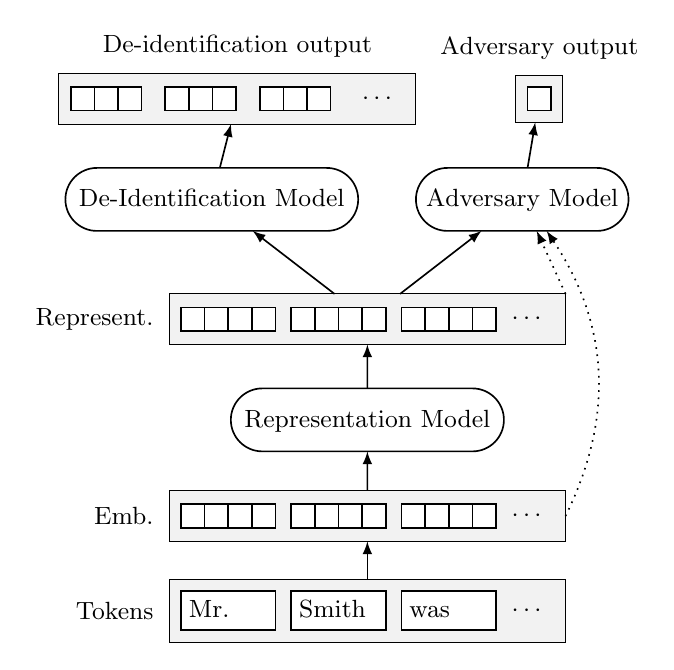
\begin{tikzpicture}[node distance=1.4cm,font=\small]
\tikzset{every node/.style={inner sep=1mm, outer sep=0mm, line width=0mm}}

\tikzstyle{token}=[rectangle,draw=black,fill=white,semithick,text width=1cm, minimum width=1.2cm, minimum height=5mm, text height=1.5ex,text depth=.25ex]
\tikzstyle{model}=[rounded rectangle,draw=black,fill=white,semithick, minimum width=3cm, minimum height=8mm, text height=1.5ex,text depth=.25ex, inner sep=1.5mm]
\tikzstyle{dots} = []
\tikzstyle{vector} = [draw, shape=rectangle, fill=white, semithick, minimum width=1.2cm, minimum height=3mm]
\tikzstyle{half vector} = [shape=rectangle, semithick, minimum width=1.2cm, minimum height=3mm] % without drawn border
\tikzstyle{two thirds vector} = [draw, shape=rectangle, fill=white, semithick, minimum width=0.9cm, minimum height=3mm]
\tikzstyle{quarter vector} = [draw, shape=rectangle, fill=white, semithick, minimum width=3mm, minimum height=3mm]
\tikzstyle{pre}=[<-,semithick, >=latex]
\tikzstyle{post}=[->, semithick, >=latex]

\node[token] (mr input){Mr.};
\node[token, right of=mr input] (smith input) {Smith};
\node[token, right of=smith input] (was input) {was};
\node[dots, right=1mm of was input] (input dots) {$\cdots$};
    
\node[vector, above=8mm of mr input] (mr embedding) {};
\node[vector, right of=mr embedding] (smith embedding) {};
\node[vector, right of=smith embedding] (was embedding) {};
\node[dots, right=1mm of was embedding] (embedding dots) {$\cdots$};

\begin{scope}[on background layer]
    \node (input box) [draw,fill=black!5,fit=(mr input) (input dots), inner sep=1.5mm] {};
    \node (feature box) [draw,fill=black!5,fit=(mr embedding) (embedding dots), inner sep=1.5mm] {};
\end{scope}

\node[model,above=5mm of feature box] (representation model) {Representation Model};

\node[vector, above=2.2cm of mr embedding] (mr representation) {};
\node[vector, right of=mr representation] (smith representation) {};
\node[vector, right of=smith representation] (was representation) {};
\node[dots, right=1mm of was representation] (representation dots) {$\cdots$};

\begin{scope}[on background layer]
    \node (representation box) [draw,fill=black!5,fit=(mr representation) (representation dots), inner sep=1.5mm] {};
\end{scope}

\node[model,above left=8mm and -2cm of representation box] (deid model) {De-Identification Model};

\node[two thirds vector, above left=2.5cm and 0.5cm of mr representation] (mr output) {};
\node[two thirds vector, right=3mm of mr output] (smith output) {};
\node[two thirds vector, right= 3mm of smith output] (was output) {};
\node[dots, right=3mm of was output] (output dots) {$\cdots$};    

\begin{scope}[on background layer]
 \node (output box) [draw,fill=black!5,fit=(mr output) (output dots), inner sep=1.5mm] {};
\end{scope}

\node[model,above right=8mm and -1.5cm of representation box] (adversary model) {Adversary Model};

\node[quarter vector, above right=2.5cm and 4mm of was representation] (adversary output) {};

\begin{scope}[on background layer]
    \node (adversary output box) [draw,fill=black!5,fit=(adversary output), inner sep=1.5mm] {};
\end{scope}


% vector squares
\foreach \i in {mr embedding, smith embedding, was embedding, mr representation, smith representation, was representation} {
    \draw[semithick] (\i.north west) rectangle ($(\i.north west) + (3mm, -3mm)$);
    \draw[semithick] (\i.north west) rectangle ($(\i.north west) + (6mm, -3mm)$);
    \draw[semithick] (\i.north west) rectangle ($(\i.north west) + (9mm, -3mm)$);    
};

\foreach \i in {mr output, smith output, was output} {
    \draw[semithick] (\i.north west) rectangle ($(\i.north west) + (3mm, -3mm)$);
    \draw[semithick] (\i.north west) rectangle ($(\i.north west) + (6mm, -3mm)$);
};

\path[post] (input box) edge (feature box);
\path[post] (feature box) edge (representation model);
\path[post] (representation model) edge (representation box);

\path[post] (representation box) edge (deid model);
\path[post] (deid model) edge (output box);

\path[post] (representation box) edge (adversary model);
\path[post,dotted] (feature box.east) edge[bend right=30] (adversary model);
\path[post,dotted] (representation box.north east) edge (adversary model);
\path[post] (adversary model) edge (adversary output box);

\node[anchor=east, left=1mm of input box] {Tokens};
\node[anchor=east, left=1mm of feature box] {Emb.};
\node[anchor=east, left=1mm of representation box] {Represent.};
\node[anchor=center, above=1mm of output box] {De-identification output};
\node[anchor=center, above=1mm of adversary output box] {Adversary output};

\end{tikzpicture}
        \caption[Adversarial model architecture]{%
            Simplified visualization of the adversarial model architecture.
            %
            Sequences of squares denote real-valued vectors, dotted arrows represent possible additional real or fake inputs to the adversary.
            %
            The casing feature that is provided as a second input to the de-identification model is omitted for legibility.}\label{fig:adversarial-model}
    \end{figure}
    
    \item[Representations]
    %
    We evaluate two types of representation models: a feedforward and \iac{lstm} model.
    %
    Both apply Gaussian noise with zero mean and trainable standard deviations to their inputs and outputs.
    %
    The models learn a standard deviation for each of the input and output dimensions.
    
    %
    We try different representation sizes to explore the trade-off between de-identification and adversary performances.
    %
    In contrast to the automatic pseudonymization approach from \cref{sec:automatic-pseudonymization} that only perturbs \ac{phi} tokens, the representation models in this approach process all tokens to represent them in a new embedding space.
    
    \item[Adversaries]
    %
    In existing gradient reversal approaches \citep{ganin2016domain,feutry2018learning,elazar2018adversarial}, the learned representation is invariant to some attribute of the input.
    %
    Similarly, our representation should be invariant to small input changes, like a single token being replaced with a neighbor in the embedding space.
    %
    The number of neighbors $N$ controls the privacy properties of the representation.
    
    %
    Additionally, we need our representation to contain a random element because we want to share the output representations as well as the representation model itself.
    %
    An attacker should not be able to create a lookup table of representations for exact sentences, i.e.\ the representation must be immune to known-plaintext attacks.
    
    %
    To achieve these goals, we use two adversaries that are trained for the following tasks:
    \begin{enumerate}
        \item Given a representation and an embedding sequence, decide if they were obtained from the same sentence.
        \item Given two representation sequences (and their cosine similarities), decide if they were obtained from the same sentence.
    \end{enumerate}
    
    %
    \Cref{fig:adversaries} shows the two adversaries with their respective inputs.
    %
    The first adversary's objective is a discriminatory formulation of an inverse representation model and causes representations for similar inputs (replacing any protected token with one of its $N$ neighbors) to be indistinguishable.
    %
    The second adversary's objective causes repeated representation computations for the same sentence to differ by a high enough degree to make it impossible to build a lookup table of representations.
    %
    We obtain the representation sequences for the second adversary from copies of the representation model with shared weights.
    %
    We generate real and fake pairs for adversarial training using the automatic pseudonymization approach presented in \cref{sec:automatic-pseudonymization}, limiting the number of replaced tokens to one per sentence.
    
    %
    The adversaries are implemented as bidirectional \ac{lstm} models.
    %
    We confirmed that bidirectional \ac{lstm} models are able to learn the adversarial tasks on randomly generated data and raw word embeddings in a preliminary experiment.
    %
    To use the two adversaries in our architecture, we average their outputs.
    
    \item[Training]
    %
    We evaluate two training procedures: \ac{dann} training~\citep{ganin2016domain} and the alternating approach by \citet{feutry2018learning}.
    
    %
    In \ac{dann} training, the three components are trained conjointly, optimizing the sum of losses.
    %
    Training the de-identification model modifies the representation model weights to generate a more meaningful representation for de-identification.
    %
    The adversary gradient is reversed with a gradient reversal layer between the adversary and the representation model in the backward pass, causing the representation to become less meaningful for the adversary.
    
    %
    The training procedure by \citet{feutry2018learning} is shown in \cref{fig:feutry-training}.
    %
    It is composed of three sequential phases:
    %
    \begin{enumerate}
        \item The de-identification and representation models are pre-trained together, optimizing the de-identification loss $L_{\text{deid}}$.
        \item The representation model is frozen and the adversary is pre-trained, optimizing the adversarial loss $L_{\text{adv}}$.
        \item In alternation, for one epoch each:
        \begin{enumerate}
            \item The representation is frozen and both de-identification model and adversary are trained, optimizing their respective losses $L_{\text{deid}}$ and $L_{\text{adv}}$.
            \item The de-identification model and adversary are frozen and the representation is trained, optimizing the combined loss $L_{\text{repr}} = L_{\text{deid}} + \lambda \abs{L_{\text{adv}} - L_{\text{random}}}$. \label{item:repr-training}
        \end{enumerate}
    \end{enumerate}
    
    \begin{figure}
        \centering
        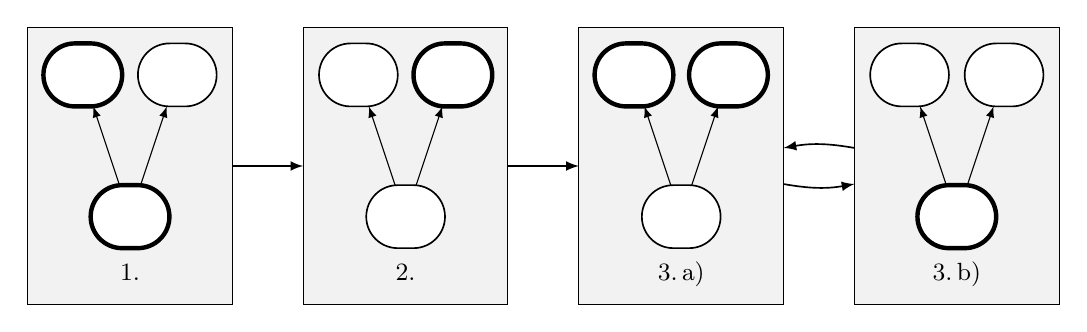
\begin{tikzpicture}[node distance=2.5cm,font=\small, sibling distance=1.2cm, level distance=1.8cm, grow=up, edge from parent/.style = {->, >=latex, draw}]
\tikzset{every node/.style={inner sep=1mm, outer sep=0mm, line width=0mm}}

\tikzstyle{model}=[rounded rectangle,draw=black,fill=white, minimum width=1.2cm, minimum height=8mm, semithick]
\tikzstyle{train}=[ultra thick]
\tikzstyle{label}=[text height=0.75ex,text depth=0ex]
\tikzstyle{dots} = []
\tikzstyle{pre}=[<-,semithick, >=latex]
\tikzstyle{post}=[->, semithick, >=latex]

\node[model, train] (a) {}
    child {node[model] (a adv) {}}
    child {node[model, train] (a deid) {}};

\node[label, below= 2mm of a] (a label) {1.}; 

\node[model, right=of a] (b) {}
    child {node[model, train] (b adv) {}}
    child {node[model] (b deid) {}};

\node[label, below=2mm of b] (b label) {2.}; 

\node[model, right=of b] (c) {}
    child {node[model, train] (c adv) {}}
    child {node[model, train] (c deid) {}};
    
\node[label, below=2mm of c] (c label) {3.$\,$a)}; 

\node[model, right= of c, train] (d) {}
    child {node[model] (d adv) {}}
    child {node[model] (d deid) {}};
    
\node[label, below=2mm of d] (d label) {3.$\,$b)}; 
    
\begin{scope}[on background layer]
    \node (a box) [draw,fill=black!5,fit=(a) (a label) (a adv) (a deid), inner sep=2mm] {};
    \node (b box) [draw,fill=black!5,fit=(b) (b label) (b adv) (b deid), inner sep=2mm] {};
    \node (c box) [draw,fill=black!5,fit=(c) (c label) (c adv) (c deid), inner sep=2mm] {};
    \node (d box) [draw,fill=black!5,fit=(d) (d label) (d adv) (d deid), inner sep=2mm] {};
\end{scope}

\path[post] (a box) edge (b box);
\path[post] (b box) edge (c box);
\path[post] (c box) edge[bend right=10] (d box);
\path[post] (d box) edge[bend right=10] (c box);

\end{tikzpicture}
        \caption[Adversarial training procedure]{%
            Visualization of \citeauthor{feutry2018learning}'s training procedure.
            %
            The adversarial model layout follows \cref{fig:adversarial-model}: the representation model is at the bottom, the left branch is the de-identification model and the right branch is the adversary.
            %
            In each step, the thick components are trained while the thin components are frozen.
            %
            Steps 1 and 2 are trained until stable.
            %
            Then training alternates between one epoch and step 3a and one epoch of step 3b.
        }\label{fig:feutry-training}
    \end{figure}
    
    %
    In the first two phases, we monitor the respective validation losses for early stopping to decide at which point the training should move on to the next phase.
    %
    The alternating steps in the third phase each last one training epoch.
    %
    We determine the early stopping epoch using only the combined validation loss (\cref{item:repr-training}).
    
    %
    Gradient reversal is achieved by optimizing the combined representation loss while the adversary weights are frozen.
    %
    The combined loss is motivated by the fact that the adversary performance should be the same as a random guessing model, which is a lower bound for anonymization~\citep{feutry2018learning}.
    %
    The term $\abs{L_{\text{adv}} - L_{\text{random}}}$ approaches $0$ when the adversary performance approaches random guessing\footnote{In the case of binary classification: $L_{\text{random}} = -\log \frac{1}{2} \approx 0.6931$.}.
    %
    $\lambda$ is a weighting factor for the two losses; we select $\lambda=1$.
    
    \item[Application]
    %
    To apply the model in practice, a central model provider would train the three parts of the model on an initial \ac{phi}-annotated dataset, e.g.\ the i2b2 2014 data.
    %
    This initial training should confirm that the learned representation allows training a de-identification model while being robust to the adversaries.
    %
    The model provider would then publish the representation model along with their choice of pre-trained word embeddings.
    %
    Medical institutions would use the representation model to transform their \ac{phi}-labeled data into a private representation, which is then sent back to the central model provider with the respective labels.
    %
    This transformation replaces the manual document-coherent pseudonymization that is typically performed to share training data for de-identification.
    
    %
    The model provider would then update the existing de-identification model or train a new model using all available representation data.
    %
    Periodically, the pipeline of representation model (possibly in a version without additive noise) and de-identification model would be published so it can be used by medical institutions on their unlabeled data.

    \item[Results]
    %
    In our adversarial learning experiment, we do not achieve satisfactory results with the conjoint \ac{dann} training procedure: in all cases, our models learn representations that are not sufficiently resistant to the adversary.
    %
    When training the adversary on the frozen representation for an additional $20$ epochs, it is able to distinguish real from fake input pairs on a test set with accuracies above $80\%$.
    %
    This confirms the findings by \citet{elazar2018adversarial}.
    
    %
    With the training procedure by \citet{feutry2018learning}, we are able to train a representation that allows training a de-identification model while preventing an adversary from learning the adversarial tasks, even with continued training on a frozen representation.
    %
    We select the \ac{lstm} representation model over the dense model because it allows $0.4$ percentage points higher de-identification \fone scores on average.
    
    %
    \Cref{fig:adversarial-deid} shows our de-identification results when using adversarially learned representations.
    %
    A higher number of neighbors $N$ means a stronger invariance requirement for the representation.
    %
    For values of $N$ up to $1\,000$, our FastText and GloVe models are able to learn representations that allow training de-identification models that reach the target \fone score of $95\%$.
    %
    However, training becomes unstable for $N>50$ when using GloVe and $N>500$ when using FastText embeddings.
    %
    Then, training results in representations that are not robust to the adversary, which is shown in the diagram on the right side.
    
    %
    Our choice of representation size $d \in \{50, 100, 300\}$ does not influence de-identifi\-ca\-tion or adversary performance, so we select $d=50$ for further evaluation.
    %
    For $d=50$ and $N=100$, the FastText model reaches an \fone score of $97.4\%$ and the GloVe model reaches an \fone score of $96.89\%$.
    
    %
    The adversarially trained FastText model beats the FastText model trained on raw data in the contact category. 
    %
    The GloVe model does not beat the corresponding raw data model in any category.
    %
    It is most significantly weaker in the profession category.
    %
    The detailed evaluation tables can be found in \cref{app:baseline-evaluation}.
\end{description}

\begin{figure*}
    \centering
    %% Creator: Matplotlib, PGF backend
%%
%% To include the figure in your LaTeX document, write
%%   \input{<filename>.pgf}
%%
%% Make sure the required packages are loaded in your preamble
%%   \usepackage{pgf}
%%
%% Figures using additional raster images can only be included by \input if
%% they are in the same directory as the main LaTeX file. For loading figures
%% from other directories you can use the `import` package
%%   \usepackage{import}
%% and then include the figures with
%%   \import{<path to file>}{<filename>.pgf}
%%
%% Matplotlib used the following preamble
%%   \usepackage{fontspec}
%%   \setmainfont{Times New Roman}
%%   \setsansfont{Lucida Grande}
%%   \setmonofont{Andale Mono}
%%
\begingroup%
\makeatletter%
\begin{pgfpicture}%
\pgfpathrectangle{\pgfpointorigin}{\pgfqpoint{5.249074in}{1.697629in}}%
\pgfusepath{use as bounding box, clip}%
\begin{pgfscope}%
\pgfsetbuttcap%
\pgfsetmiterjoin%
\definecolor{currentfill}{rgb}{1.000000,1.000000,1.000000}%
\pgfsetfillcolor{currentfill}%
\pgfsetlinewidth{0.000000pt}%
\definecolor{currentstroke}{rgb}{1.000000,1.000000,1.000000}%
\pgfsetstrokecolor{currentstroke}%
\pgfsetdash{}{0pt}%
\pgfpathmoveto{\pgfqpoint{0.000000in}{0.000000in}}%
\pgfpathlineto{\pgfqpoint{5.249074in}{0.000000in}}%
\pgfpathlineto{\pgfqpoint{5.249074in}{1.697629in}}%
\pgfpathlineto{\pgfqpoint{0.000000in}{1.697629in}}%
\pgfpathclose%
\pgfusepath{fill}%
\end{pgfscope}%
\begin{pgfscope}%
\pgfsetbuttcap%
\pgfsetmiterjoin%
\definecolor{currentfill}{rgb}{1.000000,1.000000,1.000000}%
\pgfsetfillcolor{currentfill}%
\pgfsetlinewidth{0.000000pt}%
\definecolor{currentstroke}{rgb}{0.000000,0.000000,0.000000}%
\pgfsetstrokecolor{currentstroke}%
\pgfsetstrokeopacity{0.000000}%
\pgfsetdash{}{0pt}%
\pgfpathmoveto{\pgfqpoint{0.505805in}{0.369628in}}%
\pgfpathlineto{\pgfqpoint{2.541093in}{0.369628in}}%
\pgfpathlineto{\pgfqpoint{2.541093in}{1.505517in}}%
\pgfpathlineto{\pgfqpoint{0.505805in}{1.505517in}}%
\pgfpathclose%
\pgfusepath{fill}%
\end{pgfscope}%
\begin{pgfscope}%
\pgfpathrectangle{\pgfqpoint{0.505805in}{0.369628in}}{\pgfqpoint{2.035289in}{1.135889in}}%
\pgfusepath{clip}%
\pgfsetbuttcap%
\pgfsetmiterjoin%
\definecolor{currentfill}{rgb}{0.498039,0.498039,0.498039}%
\pgfsetfillcolor{currentfill}%
\pgfsetfillopacity{0.100000}%
\pgfsetlinewidth{1.003750pt}%
\definecolor{currentstroke}{rgb}{0.498039,0.498039,0.498039}%
\pgfsetstrokecolor{currentstroke}%
\pgfsetstrokeopacity{0.100000}%
\pgfsetdash{}{0pt}%
\pgfpathmoveto{\pgfqpoint{0.501155in}{0.423718in}}%
\pgfpathlineto{\pgfqpoint{2.541093in}{0.423718in}}%
\pgfpathlineto{\pgfqpoint{2.541093in}{1.505517in}}%
\pgfpathlineto{\pgfqpoint{0.501155in}{1.505517in}}%
\pgfpathclose%
\pgfusepath{stroke,fill}%
\end{pgfscope}%
\begin{pgfscope}%
\pgfsetbuttcap%
\pgfsetroundjoin%
\definecolor{currentfill}{rgb}{0.000000,0.000000,0.000000}%
\pgfsetfillcolor{currentfill}%
\pgfsetlinewidth{0.803000pt}%
\definecolor{currentstroke}{rgb}{0.000000,0.000000,0.000000}%
\pgfsetstrokecolor{currentstroke}%
\pgfsetdash{}{0pt}%
\pgfsys@defobject{currentmarker}{\pgfqpoint{0.000000in}{-0.048611in}}{\pgfqpoint{0.000000in}{0.000000in}}{%
\pgfpathmoveto{\pgfqpoint{0.000000in}{0.000000in}}%
\pgfpathlineto{\pgfqpoint{0.000000in}{-0.048611in}}%
\pgfusepath{stroke,fill}%
}%
\begin{pgfscope}%
\pgfsys@transformshift{0.541279in}{0.369628in}%
\pgfsys@useobject{currentmarker}{}%
\end{pgfscope}%
\end{pgfscope}%
\begin{pgfscope}%
\pgftext[x=0.541279in,y=0.272406in,,top]{\sffamily\fontsize{8.000000}{9.600000}\selectfont \(\displaystyle {10^{1}}\)}%
\end{pgfscope}%
\begin{pgfscope}%
\pgfsetbuttcap%
\pgfsetroundjoin%
\definecolor{currentfill}{rgb}{0.000000,0.000000,0.000000}%
\pgfsetfillcolor{currentfill}%
\pgfsetlinewidth{0.803000pt}%
\definecolor{currentstroke}{rgb}{0.000000,0.000000,0.000000}%
\pgfsetstrokecolor{currentstroke}%
\pgfsetdash{}{0pt}%
\pgfsys@defobject{currentmarker}{\pgfqpoint{0.000000in}{-0.048611in}}{\pgfqpoint{0.000000in}{0.000000in}}{%
\pgfpathmoveto{\pgfqpoint{0.000000in}{0.000000in}}%
\pgfpathlineto{\pgfqpoint{0.000000in}{-0.048611in}}%
\pgfusepath{stroke,fill}%
}%
\begin{pgfscope}%
\pgfsys@transformshift{1.520912in}{0.369628in}%
\pgfsys@useobject{currentmarker}{}%
\end{pgfscope}%
\end{pgfscope}%
\begin{pgfscope}%
\pgftext[x=1.520912in,y=0.272406in,,top]{\sffamily\fontsize{8.000000}{9.600000}\selectfont \(\displaystyle {10^{2}}\)}%
\end{pgfscope}%
\begin{pgfscope}%
\pgfsetbuttcap%
\pgfsetroundjoin%
\definecolor{currentfill}{rgb}{0.000000,0.000000,0.000000}%
\pgfsetfillcolor{currentfill}%
\pgfsetlinewidth{0.803000pt}%
\definecolor{currentstroke}{rgb}{0.000000,0.000000,0.000000}%
\pgfsetstrokecolor{currentstroke}%
\pgfsetdash{}{0pt}%
\pgfsys@defobject{currentmarker}{\pgfqpoint{0.000000in}{-0.048611in}}{\pgfqpoint{0.000000in}{0.000000in}}{%
\pgfpathmoveto{\pgfqpoint{0.000000in}{0.000000in}}%
\pgfpathlineto{\pgfqpoint{0.000000in}{-0.048611in}}%
\pgfusepath{stroke,fill}%
}%
\begin{pgfscope}%
\pgfsys@transformshift{2.500544in}{0.369628in}%
\pgfsys@useobject{currentmarker}{}%
\end{pgfscope}%
\end{pgfscope}%
\begin{pgfscope}%
\pgftext[x=2.500544in,y=0.272406in,,top]{\sffamily\fontsize{8.000000}{9.600000}\selectfont \(\displaystyle {10^{3}}\)}%
\end{pgfscope}%
\begin{pgfscope}%
\pgfsetbuttcap%
\pgfsetroundjoin%
\definecolor{currentfill}{rgb}{0.000000,0.000000,0.000000}%
\pgfsetfillcolor{currentfill}%
\pgfsetlinewidth{0.602250pt}%
\definecolor{currentstroke}{rgb}{0.000000,0.000000,0.000000}%
\pgfsetstrokecolor{currentstroke}%
\pgfsetdash{}{0pt}%
\pgfsys@defobject{currentmarker}{\pgfqpoint{0.000000in}{-0.027778in}}{\pgfqpoint{0.000000in}{0.000000in}}{%
\pgfpathmoveto{\pgfqpoint{0.000000in}{0.000000in}}%
\pgfpathlineto{\pgfqpoint{0.000000in}{-0.027778in}}%
\pgfusepath{stroke,fill}%
}%
\begin{pgfscope}%
\pgfsys@transformshift{0.836178in}{0.369628in}%
\pgfsys@useobject{currentmarker}{}%
\end{pgfscope}%
\end{pgfscope}%
\begin{pgfscope}%
\pgfsetbuttcap%
\pgfsetroundjoin%
\definecolor{currentfill}{rgb}{0.000000,0.000000,0.000000}%
\pgfsetfillcolor{currentfill}%
\pgfsetlinewidth{0.602250pt}%
\definecolor{currentstroke}{rgb}{0.000000,0.000000,0.000000}%
\pgfsetstrokecolor{currentstroke}%
\pgfsetdash{}{0pt}%
\pgfsys@defobject{currentmarker}{\pgfqpoint{0.000000in}{-0.027778in}}{\pgfqpoint{0.000000in}{0.000000in}}{%
\pgfpathmoveto{\pgfqpoint{0.000000in}{0.000000in}}%
\pgfpathlineto{\pgfqpoint{0.000000in}{-0.027778in}}%
\pgfusepath{stroke,fill}%
}%
\begin{pgfscope}%
\pgfsys@transformshift{1.008683in}{0.369628in}%
\pgfsys@useobject{currentmarker}{}%
\end{pgfscope}%
\end{pgfscope}%
\begin{pgfscope}%
\pgfsetbuttcap%
\pgfsetroundjoin%
\definecolor{currentfill}{rgb}{0.000000,0.000000,0.000000}%
\pgfsetfillcolor{currentfill}%
\pgfsetlinewidth{0.602250pt}%
\definecolor{currentstroke}{rgb}{0.000000,0.000000,0.000000}%
\pgfsetstrokecolor{currentstroke}%
\pgfsetdash{}{0pt}%
\pgfsys@defobject{currentmarker}{\pgfqpoint{0.000000in}{-0.027778in}}{\pgfqpoint{0.000000in}{0.000000in}}{%
\pgfpathmoveto{\pgfqpoint{0.000000in}{0.000000in}}%
\pgfpathlineto{\pgfqpoint{0.000000in}{-0.027778in}}%
\pgfusepath{stroke,fill}%
}%
\begin{pgfscope}%
\pgfsys@transformshift{1.131077in}{0.369628in}%
\pgfsys@useobject{currentmarker}{}%
\end{pgfscope}%
\end{pgfscope}%
\begin{pgfscope}%
\pgfsetbuttcap%
\pgfsetroundjoin%
\definecolor{currentfill}{rgb}{0.000000,0.000000,0.000000}%
\pgfsetfillcolor{currentfill}%
\pgfsetlinewidth{0.602250pt}%
\definecolor{currentstroke}{rgb}{0.000000,0.000000,0.000000}%
\pgfsetstrokecolor{currentstroke}%
\pgfsetdash{}{0pt}%
\pgfsys@defobject{currentmarker}{\pgfqpoint{0.000000in}{-0.027778in}}{\pgfqpoint{0.000000in}{0.000000in}}{%
\pgfpathmoveto{\pgfqpoint{0.000000in}{0.000000in}}%
\pgfpathlineto{\pgfqpoint{0.000000in}{-0.027778in}}%
\pgfusepath{stroke,fill}%
}%
\begin{pgfscope}%
\pgfsys@transformshift{1.226013in}{0.369628in}%
\pgfsys@useobject{currentmarker}{}%
\end{pgfscope}%
\end{pgfscope}%
\begin{pgfscope}%
\pgfsetbuttcap%
\pgfsetroundjoin%
\definecolor{currentfill}{rgb}{0.000000,0.000000,0.000000}%
\pgfsetfillcolor{currentfill}%
\pgfsetlinewidth{0.602250pt}%
\definecolor{currentstroke}{rgb}{0.000000,0.000000,0.000000}%
\pgfsetstrokecolor{currentstroke}%
\pgfsetdash{}{0pt}%
\pgfsys@defobject{currentmarker}{\pgfqpoint{0.000000in}{-0.027778in}}{\pgfqpoint{0.000000in}{0.000000in}}{%
\pgfpathmoveto{\pgfqpoint{0.000000in}{0.000000in}}%
\pgfpathlineto{\pgfqpoint{0.000000in}{-0.027778in}}%
\pgfusepath{stroke,fill}%
}%
\begin{pgfscope}%
\pgfsys@transformshift{1.303581in}{0.369628in}%
\pgfsys@useobject{currentmarker}{}%
\end{pgfscope}%
\end{pgfscope}%
\begin{pgfscope}%
\pgfsetbuttcap%
\pgfsetroundjoin%
\definecolor{currentfill}{rgb}{0.000000,0.000000,0.000000}%
\pgfsetfillcolor{currentfill}%
\pgfsetlinewidth{0.602250pt}%
\definecolor{currentstroke}{rgb}{0.000000,0.000000,0.000000}%
\pgfsetstrokecolor{currentstroke}%
\pgfsetdash{}{0pt}%
\pgfsys@defobject{currentmarker}{\pgfqpoint{0.000000in}{-0.027778in}}{\pgfqpoint{0.000000in}{0.000000in}}{%
\pgfpathmoveto{\pgfqpoint{0.000000in}{0.000000in}}%
\pgfpathlineto{\pgfqpoint{0.000000in}{-0.027778in}}%
\pgfusepath{stroke,fill}%
}%
\begin{pgfscope}%
\pgfsys@transformshift{1.369165in}{0.369628in}%
\pgfsys@useobject{currentmarker}{}%
\end{pgfscope}%
\end{pgfscope}%
\begin{pgfscope}%
\pgfsetbuttcap%
\pgfsetroundjoin%
\definecolor{currentfill}{rgb}{0.000000,0.000000,0.000000}%
\pgfsetfillcolor{currentfill}%
\pgfsetlinewidth{0.602250pt}%
\definecolor{currentstroke}{rgb}{0.000000,0.000000,0.000000}%
\pgfsetstrokecolor{currentstroke}%
\pgfsetdash{}{0pt}%
\pgfsys@defobject{currentmarker}{\pgfqpoint{0.000000in}{-0.027778in}}{\pgfqpoint{0.000000in}{0.000000in}}{%
\pgfpathmoveto{\pgfqpoint{0.000000in}{0.000000in}}%
\pgfpathlineto{\pgfqpoint{0.000000in}{-0.027778in}}%
\pgfusepath{stroke,fill}%
}%
\begin{pgfscope}%
\pgfsys@transformshift{1.425975in}{0.369628in}%
\pgfsys@useobject{currentmarker}{}%
\end{pgfscope}%
\end{pgfscope}%
\begin{pgfscope}%
\pgfsetbuttcap%
\pgfsetroundjoin%
\definecolor{currentfill}{rgb}{0.000000,0.000000,0.000000}%
\pgfsetfillcolor{currentfill}%
\pgfsetlinewidth{0.602250pt}%
\definecolor{currentstroke}{rgb}{0.000000,0.000000,0.000000}%
\pgfsetstrokecolor{currentstroke}%
\pgfsetdash{}{0pt}%
\pgfsys@defobject{currentmarker}{\pgfqpoint{0.000000in}{-0.027778in}}{\pgfqpoint{0.000000in}{0.000000in}}{%
\pgfpathmoveto{\pgfqpoint{0.000000in}{0.000000in}}%
\pgfpathlineto{\pgfqpoint{0.000000in}{-0.027778in}}%
\pgfusepath{stroke,fill}%
}%
\begin{pgfscope}%
\pgfsys@transformshift{1.476086in}{0.369628in}%
\pgfsys@useobject{currentmarker}{}%
\end{pgfscope}%
\end{pgfscope}%
\begin{pgfscope}%
\pgfsetbuttcap%
\pgfsetroundjoin%
\definecolor{currentfill}{rgb}{0.000000,0.000000,0.000000}%
\pgfsetfillcolor{currentfill}%
\pgfsetlinewidth{0.602250pt}%
\definecolor{currentstroke}{rgb}{0.000000,0.000000,0.000000}%
\pgfsetstrokecolor{currentstroke}%
\pgfsetdash{}{0pt}%
\pgfsys@defobject{currentmarker}{\pgfqpoint{0.000000in}{-0.027778in}}{\pgfqpoint{0.000000in}{0.000000in}}{%
\pgfpathmoveto{\pgfqpoint{0.000000in}{0.000000in}}%
\pgfpathlineto{\pgfqpoint{0.000000in}{-0.027778in}}%
\pgfusepath{stroke,fill}%
}%
\begin{pgfscope}%
\pgfsys@transformshift{1.815810in}{0.369628in}%
\pgfsys@useobject{currentmarker}{}%
\end{pgfscope}%
\end{pgfscope}%
\begin{pgfscope}%
\pgfsetbuttcap%
\pgfsetroundjoin%
\definecolor{currentfill}{rgb}{0.000000,0.000000,0.000000}%
\pgfsetfillcolor{currentfill}%
\pgfsetlinewidth{0.602250pt}%
\definecolor{currentstroke}{rgb}{0.000000,0.000000,0.000000}%
\pgfsetstrokecolor{currentstroke}%
\pgfsetdash{}{0pt}%
\pgfsys@defobject{currentmarker}{\pgfqpoint{0.000000in}{-0.027778in}}{\pgfqpoint{0.000000in}{0.000000in}}{%
\pgfpathmoveto{\pgfqpoint{0.000000in}{0.000000in}}%
\pgfpathlineto{\pgfqpoint{0.000000in}{-0.027778in}}%
\pgfusepath{stroke,fill}%
}%
\begin{pgfscope}%
\pgfsys@transformshift{1.988315in}{0.369628in}%
\pgfsys@useobject{currentmarker}{}%
\end{pgfscope}%
\end{pgfscope}%
\begin{pgfscope}%
\pgfsetbuttcap%
\pgfsetroundjoin%
\definecolor{currentfill}{rgb}{0.000000,0.000000,0.000000}%
\pgfsetfillcolor{currentfill}%
\pgfsetlinewidth{0.602250pt}%
\definecolor{currentstroke}{rgb}{0.000000,0.000000,0.000000}%
\pgfsetstrokecolor{currentstroke}%
\pgfsetdash{}{0pt}%
\pgfsys@defobject{currentmarker}{\pgfqpoint{0.000000in}{-0.027778in}}{\pgfqpoint{0.000000in}{0.000000in}}{%
\pgfpathmoveto{\pgfqpoint{0.000000in}{0.000000in}}%
\pgfpathlineto{\pgfqpoint{0.000000in}{-0.027778in}}%
\pgfusepath{stroke,fill}%
}%
\begin{pgfscope}%
\pgfsys@transformshift{2.110709in}{0.369628in}%
\pgfsys@useobject{currentmarker}{}%
\end{pgfscope}%
\end{pgfscope}%
\begin{pgfscope}%
\pgfsetbuttcap%
\pgfsetroundjoin%
\definecolor{currentfill}{rgb}{0.000000,0.000000,0.000000}%
\pgfsetfillcolor{currentfill}%
\pgfsetlinewidth{0.602250pt}%
\definecolor{currentstroke}{rgb}{0.000000,0.000000,0.000000}%
\pgfsetstrokecolor{currentstroke}%
\pgfsetdash{}{0pt}%
\pgfsys@defobject{currentmarker}{\pgfqpoint{0.000000in}{-0.027778in}}{\pgfqpoint{0.000000in}{0.000000in}}{%
\pgfpathmoveto{\pgfqpoint{0.000000in}{0.000000in}}%
\pgfpathlineto{\pgfqpoint{0.000000in}{-0.027778in}}%
\pgfusepath{stroke,fill}%
}%
\begin{pgfscope}%
\pgfsys@transformshift{2.205645in}{0.369628in}%
\pgfsys@useobject{currentmarker}{}%
\end{pgfscope}%
\end{pgfscope}%
\begin{pgfscope}%
\pgfsetbuttcap%
\pgfsetroundjoin%
\definecolor{currentfill}{rgb}{0.000000,0.000000,0.000000}%
\pgfsetfillcolor{currentfill}%
\pgfsetlinewidth{0.602250pt}%
\definecolor{currentstroke}{rgb}{0.000000,0.000000,0.000000}%
\pgfsetstrokecolor{currentstroke}%
\pgfsetdash{}{0pt}%
\pgfsys@defobject{currentmarker}{\pgfqpoint{0.000000in}{-0.027778in}}{\pgfqpoint{0.000000in}{0.000000in}}{%
\pgfpathmoveto{\pgfqpoint{0.000000in}{0.000000in}}%
\pgfpathlineto{\pgfqpoint{0.000000in}{-0.027778in}}%
\pgfusepath{stroke,fill}%
}%
\begin{pgfscope}%
\pgfsys@transformshift{2.283214in}{0.369628in}%
\pgfsys@useobject{currentmarker}{}%
\end{pgfscope}%
\end{pgfscope}%
\begin{pgfscope}%
\pgfsetbuttcap%
\pgfsetroundjoin%
\definecolor{currentfill}{rgb}{0.000000,0.000000,0.000000}%
\pgfsetfillcolor{currentfill}%
\pgfsetlinewidth{0.602250pt}%
\definecolor{currentstroke}{rgb}{0.000000,0.000000,0.000000}%
\pgfsetstrokecolor{currentstroke}%
\pgfsetdash{}{0pt}%
\pgfsys@defobject{currentmarker}{\pgfqpoint{0.000000in}{-0.027778in}}{\pgfqpoint{0.000000in}{0.000000in}}{%
\pgfpathmoveto{\pgfqpoint{0.000000in}{0.000000in}}%
\pgfpathlineto{\pgfqpoint{0.000000in}{-0.027778in}}%
\pgfusepath{stroke,fill}%
}%
\begin{pgfscope}%
\pgfsys@transformshift{2.348797in}{0.369628in}%
\pgfsys@useobject{currentmarker}{}%
\end{pgfscope}%
\end{pgfscope}%
\begin{pgfscope}%
\pgfsetbuttcap%
\pgfsetroundjoin%
\definecolor{currentfill}{rgb}{0.000000,0.000000,0.000000}%
\pgfsetfillcolor{currentfill}%
\pgfsetlinewidth{0.602250pt}%
\definecolor{currentstroke}{rgb}{0.000000,0.000000,0.000000}%
\pgfsetstrokecolor{currentstroke}%
\pgfsetdash{}{0pt}%
\pgfsys@defobject{currentmarker}{\pgfqpoint{0.000000in}{-0.027778in}}{\pgfqpoint{0.000000in}{0.000000in}}{%
\pgfpathmoveto{\pgfqpoint{0.000000in}{0.000000in}}%
\pgfpathlineto{\pgfqpoint{0.000000in}{-0.027778in}}%
\pgfusepath{stroke,fill}%
}%
\begin{pgfscope}%
\pgfsys@transformshift{2.405608in}{0.369628in}%
\pgfsys@useobject{currentmarker}{}%
\end{pgfscope}%
\end{pgfscope}%
\begin{pgfscope}%
\pgfsetbuttcap%
\pgfsetroundjoin%
\definecolor{currentfill}{rgb}{0.000000,0.000000,0.000000}%
\pgfsetfillcolor{currentfill}%
\pgfsetlinewidth{0.602250pt}%
\definecolor{currentstroke}{rgb}{0.000000,0.000000,0.000000}%
\pgfsetstrokecolor{currentstroke}%
\pgfsetdash{}{0pt}%
\pgfsys@defobject{currentmarker}{\pgfqpoint{0.000000in}{-0.027778in}}{\pgfqpoint{0.000000in}{0.000000in}}{%
\pgfpathmoveto{\pgfqpoint{0.000000in}{0.000000in}}%
\pgfpathlineto{\pgfqpoint{0.000000in}{-0.027778in}}%
\pgfusepath{stroke,fill}%
}%
\begin{pgfscope}%
\pgfsys@transformshift{2.455718in}{0.369628in}%
\pgfsys@useobject{currentmarker}{}%
\end{pgfscope}%
\end{pgfscope}%
\begin{pgfscope}%
\pgftext[x=1.523449in,y=0.109755in,,top]{\sffamily\fontsize{8.000000}{9.600000}\selectfont Number of neighbors \(\displaystyle N\)}%
\end{pgfscope}%
\begin{pgfscope}%
\pgfsetbuttcap%
\pgfsetroundjoin%
\definecolor{currentfill}{rgb}{0.000000,0.000000,0.000000}%
\pgfsetfillcolor{currentfill}%
\pgfsetlinewidth{0.803000pt}%
\definecolor{currentstroke}{rgb}{0.000000,0.000000,0.000000}%
\pgfsetstrokecolor{currentstroke}%
\pgfsetdash{}{0pt}%
\pgfsys@defobject{currentmarker}{\pgfqpoint{-0.048611in}{0.000000in}}{\pgfqpoint{0.000000in}{0.000000in}}{%
\pgfpathmoveto{\pgfqpoint{0.000000in}{0.000000in}}%
\pgfpathlineto{\pgfqpoint{-0.048611in}{0.000000in}}%
\pgfusepath{stroke,fill}%
}%
\begin{pgfscope}%
\pgfsys@transformshift{0.505805in}{0.640078in}%
\pgfsys@useobject{currentmarker}{}%
\end{pgfscope}%
\end{pgfscope}%
\begin{pgfscope}%
\pgftext[x=0.162652in,y=0.597245in,left,base]{\sffamily\fontsize{8.000000}{9.600000}\selectfont 0.96}%
\end{pgfscope}%
\begin{pgfscope}%
\pgfsetbuttcap%
\pgfsetroundjoin%
\definecolor{currentfill}{rgb}{0.000000,0.000000,0.000000}%
\pgfsetfillcolor{currentfill}%
\pgfsetlinewidth{0.803000pt}%
\definecolor{currentstroke}{rgb}{0.000000,0.000000,0.000000}%
\pgfsetstrokecolor{currentstroke}%
\pgfsetdash{}{0pt}%
\pgfsys@defobject{currentmarker}{\pgfqpoint{-0.048611in}{0.000000in}}{\pgfqpoint{0.000000in}{0.000000in}}{%
\pgfpathmoveto{\pgfqpoint{0.000000in}{0.000000in}}%
\pgfpathlineto{\pgfqpoint{-0.048611in}{0.000000in}}%
\pgfusepath{stroke,fill}%
}%
\begin{pgfscope}%
\pgfsys@transformshift{0.505805in}{1.072798in}%
\pgfsys@useobject{currentmarker}{}%
\end{pgfscope}%
\end{pgfscope}%
\begin{pgfscope}%
\pgftext[x=0.162652in,y=1.029965in,left,base]{\sffamily\fontsize{8.000000}{9.600000}\selectfont 0.98}%
\end{pgfscope}%
\begin{pgfscope}%
\pgfsetbuttcap%
\pgfsetroundjoin%
\definecolor{currentfill}{rgb}{0.000000,0.000000,0.000000}%
\pgfsetfillcolor{currentfill}%
\pgfsetlinewidth{0.803000pt}%
\definecolor{currentstroke}{rgb}{0.000000,0.000000,0.000000}%
\pgfsetstrokecolor{currentstroke}%
\pgfsetdash{}{0pt}%
\pgfsys@defobject{currentmarker}{\pgfqpoint{-0.048611in}{0.000000in}}{\pgfqpoint{0.000000in}{0.000000in}}{%
\pgfpathmoveto{\pgfqpoint{0.000000in}{0.000000in}}%
\pgfpathlineto{\pgfqpoint{-0.048611in}{0.000000in}}%
\pgfusepath{stroke,fill}%
}%
\begin{pgfscope}%
\pgfsys@transformshift{0.505805in}{1.505517in}%
\pgfsys@useobject{currentmarker}{}%
\end{pgfscope}%
\end{pgfscope}%
\begin{pgfscope}%
\pgftext[x=0.162652in,y=1.462684in,left,base]{\sffamily\fontsize{8.000000}{9.600000}\selectfont 1.00}%
\end{pgfscope}%
\begin{pgfscope}%
\pgftext[x=0.107096in,y=0.937573in,,bottom,rotate=90.000000]{\sffamily\fontsize{8.000000}{9.600000}\selectfont Binary HIPAA F1 score}%
\end{pgfscope}%
\begin{pgfscope}%
\pgfpathrectangle{\pgfqpoint{0.505805in}{0.369628in}}{\pgfqpoint{2.035289in}{1.135889in}}%
\pgfusepath{clip}%
\pgfsetrectcap%
\pgfsetroundjoin%
\pgfsetlinewidth{1.505625pt}%
\definecolor{currentstroke}{rgb}{0.121569,0.466667,0.705882}%
\pgfsetstrokecolor{currentstroke}%
\pgfsetdash{}{0pt}%
\pgfpathmoveto{\pgfqpoint{0.541279in}{0.888892in}}%
\pgfpathlineto{\pgfqpoint{0.836178in}{0.945146in}}%
\pgfpathlineto{\pgfqpoint{1.226013in}{0.934328in}}%
\pgfpathlineto{\pgfqpoint{1.520912in}{0.942982in}}%
\pgfpathlineto{\pgfqpoint{1.815810in}{0.921346in}}%
\pgfpathlineto{\pgfqpoint{2.205645in}{0.932164in}}%
\pgfpathlineto{\pgfqpoint{2.500544in}{0.802348in}}%
\pgfusepath{stroke}%
\end{pgfscope}%
\begin{pgfscope}%
\pgfpathrectangle{\pgfqpoint{0.505805in}{0.369628in}}{\pgfqpoint{2.035289in}{1.135889in}}%
\pgfusepath{clip}%
\pgfsetbuttcap%
\pgfsetroundjoin%
\definecolor{currentfill}{rgb}{0.121569,0.466667,0.705882}%
\pgfsetfillcolor{currentfill}%
\pgfsetlinewidth{1.003750pt}%
\definecolor{currentstroke}{rgb}{0.121569,0.466667,0.705882}%
\pgfsetstrokecolor{currentstroke}%
\pgfsetdash{}{0pt}%
\pgfsys@defobject{currentmarker}{\pgfqpoint{-0.020833in}{-0.020833in}}{\pgfqpoint{0.020833in}{0.020833in}}{%
\pgfpathmoveto{\pgfqpoint{0.000000in}{-0.020833in}}%
\pgfpathcurveto{\pgfqpoint{0.005525in}{-0.020833in}}{\pgfqpoint{0.010825in}{-0.018638in}}{\pgfqpoint{0.014731in}{-0.014731in}}%
\pgfpathcurveto{\pgfqpoint{0.018638in}{-0.010825in}}{\pgfqpoint{0.020833in}{-0.005525in}}{\pgfqpoint{0.020833in}{0.000000in}}%
\pgfpathcurveto{\pgfqpoint{0.020833in}{0.005525in}}{\pgfqpoint{0.018638in}{0.010825in}}{\pgfqpoint{0.014731in}{0.014731in}}%
\pgfpathcurveto{\pgfqpoint{0.010825in}{0.018638in}}{\pgfqpoint{0.005525in}{0.020833in}}{\pgfqpoint{0.000000in}{0.020833in}}%
\pgfpathcurveto{\pgfqpoint{-0.005525in}{0.020833in}}{\pgfqpoint{-0.010825in}{0.018638in}}{\pgfqpoint{-0.014731in}{0.014731in}}%
\pgfpathcurveto{\pgfqpoint{-0.018638in}{0.010825in}}{\pgfqpoint{-0.020833in}{0.005525in}}{\pgfqpoint{-0.020833in}{0.000000in}}%
\pgfpathcurveto{\pgfqpoint{-0.020833in}{-0.005525in}}{\pgfqpoint{-0.018638in}{-0.010825in}}{\pgfqpoint{-0.014731in}{-0.014731in}}%
\pgfpathcurveto{\pgfqpoint{-0.010825in}{-0.018638in}}{\pgfqpoint{-0.005525in}{-0.020833in}}{\pgfqpoint{0.000000in}{-0.020833in}}%
\pgfpathclose%
\pgfusepath{stroke,fill}%
}%
\begin{pgfscope}%
\pgfsys@transformshift{0.541279in}{0.888892in}%
\pgfsys@useobject{currentmarker}{}%
\end{pgfscope}%
\begin{pgfscope}%
\pgfsys@transformshift{0.836178in}{0.945146in}%
\pgfsys@useobject{currentmarker}{}%
\end{pgfscope}%
\begin{pgfscope}%
\pgfsys@transformshift{1.226013in}{0.934328in}%
\pgfsys@useobject{currentmarker}{}%
\end{pgfscope}%
\begin{pgfscope}%
\pgfsys@transformshift{1.520912in}{0.942982in}%
\pgfsys@useobject{currentmarker}{}%
\end{pgfscope}%
\begin{pgfscope}%
\pgfsys@transformshift{1.815810in}{0.921346in}%
\pgfsys@useobject{currentmarker}{}%
\end{pgfscope}%
\begin{pgfscope}%
\pgfsys@transformshift{2.205645in}{0.932164in}%
\pgfsys@useobject{currentmarker}{}%
\end{pgfscope}%
\begin{pgfscope}%
\pgfsys@transformshift{2.500544in}{0.802348in}%
\pgfsys@useobject{currentmarker}{}%
\end{pgfscope}%
\end{pgfscope}%
\begin{pgfscope}%
\pgfpathrectangle{\pgfqpoint{0.505805in}{0.369628in}}{\pgfqpoint{2.035289in}{1.135889in}}%
\pgfusepath{clip}%
\pgfsetrectcap%
\pgfsetroundjoin%
\pgfsetlinewidth{1.505625pt}%
\definecolor{currentstroke}{rgb}{1.000000,0.498039,0.054902}%
\pgfsetstrokecolor{currentstroke}%
\pgfsetdash{}{0pt}%
\pgfpathmoveto{\pgfqpoint{0.541279in}{0.884565in}}%
\pgfpathlineto{\pgfqpoint{0.836178in}{0.808839in}}%
\pgfpathlineto{\pgfqpoint{1.226013in}{0.769894in}}%
\pgfpathlineto{\pgfqpoint{1.520912in}{0.832638in}}%
\pgfpathlineto{\pgfqpoint{1.815810in}{0.748258in}}%
\pgfpathlineto{\pgfqpoint{2.205645in}{0.717968in}}%
\pgfpathlineto{\pgfqpoint{2.500544in}{0.804512in}}%
\pgfusepath{stroke}%
\end{pgfscope}%
\begin{pgfscope}%
\pgfpathrectangle{\pgfqpoint{0.505805in}{0.369628in}}{\pgfqpoint{2.035289in}{1.135889in}}%
\pgfusepath{clip}%
\pgfsetbuttcap%
\pgfsetroundjoin%
\definecolor{currentfill}{rgb}{1.000000,0.498039,0.054902}%
\pgfsetfillcolor{currentfill}%
\pgfsetlinewidth{1.003750pt}%
\definecolor{currentstroke}{rgb}{1.000000,0.498039,0.054902}%
\pgfsetstrokecolor{currentstroke}%
\pgfsetdash{}{0pt}%
\pgfsys@defobject{currentmarker}{\pgfqpoint{-0.020833in}{-0.020833in}}{\pgfqpoint{0.020833in}{0.020833in}}{%
\pgfpathmoveto{\pgfqpoint{0.000000in}{-0.020833in}}%
\pgfpathcurveto{\pgfqpoint{0.005525in}{-0.020833in}}{\pgfqpoint{0.010825in}{-0.018638in}}{\pgfqpoint{0.014731in}{-0.014731in}}%
\pgfpathcurveto{\pgfqpoint{0.018638in}{-0.010825in}}{\pgfqpoint{0.020833in}{-0.005525in}}{\pgfqpoint{0.020833in}{0.000000in}}%
\pgfpathcurveto{\pgfqpoint{0.020833in}{0.005525in}}{\pgfqpoint{0.018638in}{0.010825in}}{\pgfqpoint{0.014731in}{0.014731in}}%
\pgfpathcurveto{\pgfqpoint{0.010825in}{0.018638in}}{\pgfqpoint{0.005525in}{0.020833in}}{\pgfqpoint{0.000000in}{0.020833in}}%
\pgfpathcurveto{\pgfqpoint{-0.005525in}{0.020833in}}{\pgfqpoint{-0.010825in}{0.018638in}}{\pgfqpoint{-0.014731in}{0.014731in}}%
\pgfpathcurveto{\pgfqpoint{-0.018638in}{0.010825in}}{\pgfqpoint{-0.020833in}{0.005525in}}{\pgfqpoint{-0.020833in}{0.000000in}}%
\pgfpathcurveto{\pgfqpoint{-0.020833in}{-0.005525in}}{\pgfqpoint{-0.018638in}{-0.010825in}}{\pgfqpoint{-0.014731in}{-0.014731in}}%
\pgfpathcurveto{\pgfqpoint{-0.010825in}{-0.018638in}}{\pgfqpoint{-0.005525in}{-0.020833in}}{\pgfqpoint{0.000000in}{-0.020833in}}%
\pgfpathclose%
\pgfusepath{stroke,fill}%
}%
\begin{pgfscope}%
\pgfsys@transformshift{0.541279in}{0.884565in}%
\pgfsys@useobject{currentmarker}{}%
\end{pgfscope}%
\begin{pgfscope}%
\pgfsys@transformshift{0.836178in}{0.808839in}%
\pgfsys@useobject{currentmarker}{}%
\end{pgfscope}%
\begin{pgfscope}%
\pgfsys@transformshift{1.226013in}{0.769894in}%
\pgfsys@useobject{currentmarker}{}%
\end{pgfscope}%
\begin{pgfscope}%
\pgfsys@transformshift{1.520912in}{0.832638in}%
\pgfsys@useobject{currentmarker}{}%
\end{pgfscope}%
\begin{pgfscope}%
\pgfsys@transformshift{1.815810in}{0.748258in}%
\pgfsys@useobject{currentmarker}{}%
\end{pgfscope}%
\begin{pgfscope}%
\pgfsys@transformshift{2.205645in}{0.717968in}%
\pgfsys@useobject{currentmarker}{}%
\end{pgfscope}%
\begin{pgfscope}%
\pgfsys@transformshift{2.500544in}{0.804512in}%
\pgfsys@useobject{currentmarker}{}%
\end{pgfscope}%
\end{pgfscope}%
\begin{pgfscope}%
\pgfpathrectangle{\pgfqpoint{0.505805in}{0.369628in}}{\pgfqpoint{2.035289in}{1.135889in}}%
\pgfusepath{clip}%
\pgfsetbuttcap%
\pgfsetroundjoin%
\pgfsetlinewidth{1.505625pt}%
\definecolor{currentstroke}{rgb}{0.498039,0.498039,0.498039}%
\pgfsetstrokecolor{currentstroke}%
\pgfsetdash{{5.550000pt}{2.400000pt}}{0.000000pt}%
\pgfpathmoveto{\pgfqpoint{0.505805in}{0.423718in}}%
\pgfpathlineto{\pgfqpoint{2.541093in}{0.423718in}}%
\pgfusepath{stroke}%
\end{pgfscope}%
\begin{pgfscope}%
\pgfsetrectcap%
\pgfsetmiterjoin%
\pgfsetlinewidth{0.803000pt}%
\definecolor{currentstroke}{rgb}{0.000000,0.000000,0.000000}%
\pgfsetstrokecolor{currentstroke}%
\pgfsetdash{}{0pt}%
\pgfpathmoveto{\pgfqpoint{0.505805in}{0.369628in}}%
\pgfpathlineto{\pgfqpoint{0.505805in}{1.505517in}}%
\pgfusepath{stroke}%
\end{pgfscope}%
\begin{pgfscope}%
\pgfsetrectcap%
\pgfsetmiterjoin%
\pgfsetlinewidth{0.803000pt}%
\definecolor{currentstroke}{rgb}{0.000000,0.000000,0.000000}%
\pgfsetstrokecolor{currentstroke}%
\pgfsetdash{}{0pt}%
\pgfpathmoveto{\pgfqpoint{2.541093in}{0.369628in}}%
\pgfpathlineto{\pgfqpoint{2.541093in}{1.505517in}}%
\pgfusepath{stroke}%
\end{pgfscope}%
\begin{pgfscope}%
\pgfsetrectcap%
\pgfsetmiterjoin%
\pgfsetlinewidth{0.803000pt}%
\definecolor{currentstroke}{rgb}{0.000000,0.000000,0.000000}%
\pgfsetstrokecolor{currentstroke}%
\pgfsetdash{}{0pt}%
\pgfpathmoveto{\pgfqpoint{0.505805in}{0.369628in}}%
\pgfpathlineto{\pgfqpoint{2.541093in}{0.369628in}}%
\pgfusepath{stroke}%
\end{pgfscope}%
\begin{pgfscope}%
\pgfsetrectcap%
\pgfsetmiterjoin%
\pgfsetlinewidth{0.803000pt}%
\definecolor{currentstroke}{rgb}{0.000000,0.000000,0.000000}%
\pgfsetstrokecolor{currentstroke}%
\pgfsetdash{}{0pt}%
\pgfpathmoveto{\pgfqpoint{0.505805in}{1.505517in}}%
\pgfpathlineto{\pgfqpoint{2.541093in}{1.505517in}}%
\pgfusepath{stroke}%
\end{pgfscope}%
\begin{pgfscope}%
\pgftext[x=1.523449in,y=1.588851in,,base]{\sffamily\fontsize{10.000000}{12.000000}\selectfont De-identification performance}%
\end{pgfscope}%
\begin{pgfscope}%
\pgfsetbuttcap%
\pgfsetmiterjoin%
\definecolor{currentfill}{rgb}{1.000000,1.000000,1.000000}%
\pgfsetfillcolor{currentfill}%
\pgfsetlinewidth{0.000000pt}%
\definecolor{currentstroke}{rgb}{0.000000,0.000000,0.000000}%
\pgfsetstrokecolor{currentstroke}%
\pgfsetstrokeopacity{0.000000}%
\pgfsetdash{}{0pt}%
\pgfpathmoveto{\pgfqpoint{3.166371in}{0.369628in}}%
\pgfpathlineto{\pgfqpoint{5.201660in}{0.369628in}}%
\pgfpathlineto{\pgfqpoint{5.201660in}{1.505517in}}%
\pgfpathlineto{\pgfqpoint{3.166371in}{1.505517in}}%
\pgfpathclose%
\pgfusepath{fill}%
\end{pgfscope}%
\begin{pgfscope}%
\pgfsetbuttcap%
\pgfsetroundjoin%
\definecolor{currentfill}{rgb}{0.000000,0.000000,0.000000}%
\pgfsetfillcolor{currentfill}%
\pgfsetlinewidth{0.803000pt}%
\definecolor{currentstroke}{rgb}{0.000000,0.000000,0.000000}%
\pgfsetstrokecolor{currentstroke}%
\pgfsetdash{}{0pt}%
\pgfsys@defobject{currentmarker}{\pgfqpoint{0.000000in}{-0.048611in}}{\pgfqpoint{0.000000in}{0.000000in}}{%
\pgfpathmoveto{\pgfqpoint{0.000000in}{0.000000in}}%
\pgfpathlineto{\pgfqpoint{0.000000in}{-0.048611in}}%
\pgfusepath{stroke,fill}%
}%
\begin{pgfscope}%
\pgfsys@transformshift{3.201846in}{0.369628in}%
\pgfsys@useobject{currentmarker}{}%
\end{pgfscope}%
\end{pgfscope}%
\begin{pgfscope}%
\pgftext[x=3.201846in,y=0.272406in,,top]{\sffamily\fontsize{8.000000}{9.600000}\selectfont \(\displaystyle {10^{1}}\)}%
\end{pgfscope}%
\begin{pgfscope}%
\pgfsetbuttcap%
\pgfsetroundjoin%
\definecolor{currentfill}{rgb}{0.000000,0.000000,0.000000}%
\pgfsetfillcolor{currentfill}%
\pgfsetlinewidth{0.803000pt}%
\definecolor{currentstroke}{rgb}{0.000000,0.000000,0.000000}%
\pgfsetstrokecolor{currentstroke}%
\pgfsetdash{}{0pt}%
\pgfsys@defobject{currentmarker}{\pgfqpoint{0.000000in}{-0.048611in}}{\pgfqpoint{0.000000in}{0.000000in}}{%
\pgfpathmoveto{\pgfqpoint{0.000000in}{0.000000in}}%
\pgfpathlineto{\pgfqpoint{0.000000in}{-0.048611in}}%
\pgfusepath{stroke,fill}%
}%
\begin{pgfscope}%
\pgfsys@transformshift{4.181478in}{0.369628in}%
\pgfsys@useobject{currentmarker}{}%
\end{pgfscope}%
\end{pgfscope}%
\begin{pgfscope}%
\pgftext[x=4.181478in,y=0.272406in,,top]{\sffamily\fontsize{8.000000}{9.600000}\selectfont \(\displaystyle {10^{2}}\)}%
\end{pgfscope}%
\begin{pgfscope}%
\pgfsetbuttcap%
\pgfsetroundjoin%
\definecolor{currentfill}{rgb}{0.000000,0.000000,0.000000}%
\pgfsetfillcolor{currentfill}%
\pgfsetlinewidth{0.803000pt}%
\definecolor{currentstroke}{rgb}{0.000000,0.000000,0.000000}%
\pgfsetstrokecolor{currentstroke}%
\pgfsetdash{}{0pt}%
\pgfsys@defobject{currentmarker}{\pgfqpoint{0.000000in}{-0.048611in}}{\pgfqpoint{0.000000in}{0.000000in}}{%
\pgfpathmoveto{\pgfqpoint{0.000000in}{0.000000in}}%
\pgfpathlineto{\pgfqpoint{0.000000in}{-0.048611in}}%
\pgfusepath{stroke,fill}%
}%
\begin{pgfscope}%
\pgfsys@transformshift{5.161110in}{0.369628in}%
\pgfsys@useobject{currentmarker}{}%
\end{pgfscope}%
\end{pgfscope}%
\begin{pgfscope}%
\pgftext[x=5.161110in,y=0.272406in,,top]{\sffamily\fontsize{8.000000}{9.600000}\selectfont \(\displaystyle {10^{3}}\)}%
\end{pgfscope}%
\begin{pgfscope}%
\pgfsetbuttcap%
\pgfsetroundjoin%
\definecolor{currentfill}{rgb}{0.000000,0.000000,0.000000}%
\pgfsetfillcolor{currentfill}%
\pgfsetlinewidth{0.602250pt}%
\definecolor{currentstroke}{rgb}{0.000000,0.000000,0.000000}%
\pgfsetstrokecolor{currentstroke}%
\pgfsetdash{}{0pt}%
\pgfsys@defobject{currentmarker}{\pgfqpoint{0.000000in}{-0.027778in}}{\pgfqpoint{0.000000in}{0.000000in}}{%
\pgfpathmoveto{\pgfqpoint{0.000000in}{0.000000in}}%
\pgfpathlineto{\pgfqpoint{0.000000in}{-0.027778in}}%
\pgfusepath{stroke,fill}%
}%
\begin{pgfscope}%
\pgfsys@transformshift{3.496744in}{0.369628in}%
\pgfsys@useobject{currentmarker}{}%
\end{pgfscope}%
\end{pgfscope}%
\begin{pgfscope}%
\pgfsetbuttcap%
\pgfsetroundjoin%
\definecolor{currentfill}{rgb}{0.000000,0.000000,0.000000}%
\pgfsetfillcolor{currentfill}%
\pgfsetlinewidth{0.602250pt}%
\definecolor{currentstroke}{rgb}{0.000000,0.000000,0.000000}%
\pgfsetstrokecolor{currentstroke}%
\pgfsetdash{}{0pt}%
\pgfsys@defobject{currentmarker}{\pgfqpoint{0.000000in}{-0.027778in}}{\pgfqpoint{0.000000in}{0.000000in}}{%
\pgfpathmoveto{\pgfqpoint{0.000000in}{0.000000in}}%
\pgfpathlineto{\pgfqpoint{0.000000in}{-0.027778in}}%
\pgfusepath{stroke,fill}%
}%
\begin{pgfscope}%
\pgfsys@transformshift{3.669249in}{0.369628in}%
\pgfsys@useobject{currentmarker}{}%
\end{pgfscope}%
\end{pgfscope}%
\begin{pgfscope}%
\pgfsetbuttcap%
\pgfsetroundjoin%
\definecolor{currentfill}{rgb}{0.000000,0.000000,0.000000}%
\pgfsetfillcolor{currentfill}%
\pgfsetlinewidth{0.602250pt}%
\definecolor{currentstroke}{rgb}{0.000000,0.000000,0.000000}%
\pgfsetstrokecolor{currentstroke}%
\pgfsetdash{}{0pt}%
\pgfsys@defobject{currentmarker}{\pgfqpoint{0.000000in}{-0.027778in}}{\pgfqpoint{0.000000in}{0.000000in}}{%
\pgfpathmoveto{\pgfqpoint{0.000000in}{0.000000in}}%
\pgfpathlineto{\pgfqpoint{0.000000in}{-0.027778in}}%
\pgfusepath{stroke,fill}%
}%
\begin{pgfscope}%
\pgfsys@transformshift{3.791643in}{0.369628in}%
\pgfsys@useobject{currentmarker}{}%
\end{pgfscope}%
\end{pgfscope}%
\begin{pgfscope}%
\pgfsetbuttcap%
\pgfsetroundjoin%
\definecolor{currentfill}{rgb}{0.000000,0.000000,0.000000}%
\pgfsetfillcolor{currentfill}%
\pgfsetlinewidth{0.602250pt}%
\definecolor{currentstroke}{rgb}{0.000000,0.000000,0.000000}%
\pgfsetstrokecolor{currentstroke}%
\pgfsetdash{}{0pt}%
\pgfsys@defobject{currentmarker}{\pgfqpoint{0.000000in}{-0.027778in}}{\pgfqpoint{0.000000in}{0.000000in}}{%
\pgfpathmoveto{\pgfqpoint{0.000000in}{0.000000in}}%
\pgfpathlineto{\pgfqpoint{0.000000in}{-0.027778in}}%
\pgfusepath{stroke,fill}%
}%
\begin{pgfscope}%
\pgfsys@transformshift{3.886579in}{0.369628in}%
\pgfsys@useobject{currentmarker}{}%
\end{pgfscope}%
\end{pgfscope}%
\begin{pgfscope}%
\pgfsetbuttcap%
\pgfsetroundjoin%
\definecolor{currentfill}{rgb}{0.000000,0.000000,0.000000}%
\pgfsetfillcolor{currentfill}%
\pgfsetlinewidth{0.602250pt}%
\definecolor{currentstroke}{rgb}{0.000000,0.000000,0.000000}%
\pgfsetstrokecolor{currentstroke}%
\pgfsetdash{}{0pt}%
\pgfsys@defobject{currentmarker}{\pgfqpoint{0.000000in}{-0.027778in}}{\pgfqpoint{0.000000in}{0.000000in}}{%
\pgfpathmoveto{\pgfqpoint{0.000000in}{0.000000in}}%
\pgfpathlineto{\pgfqpoint{0.000000in}{-0.027778in}}%
\pgfusepath{stroke,fill}%
}%
\begin{pgfscope}%
\pgfsys@transformshift{3.964148in}{0.369628in}%
\pgfsys@useobject{currentmarker}{}%
\end{pgfscope}%
\end{pgfscope}%
\begin{pgfscope}%
\pgfsetbuttcap%
\pgfsetroundjoin%
\definecolor{currentfill}{rgb}{0.000000,0.000000,0.000000}%
\pgfsetfillcolor{currentfill}%
\pgfsetlinewidth{0.602250pt}%
\definecolor{currentstroke}{rgb}{0.000000,0.000000,0.000000}%
\pgfsetstrokecolor{currentstroke}%
\pgfsetdash{}{0pt}%
\pgfsys@defobject{currentmarker}{\pgfqpoint{0.000000in}{-0.027778in}}{\pgfqpoint{0.000000in}{0.000000in}}{%
\pgfpathmoveto{\pgfqpoint{0.000000in}{0.000000in}}%
\pgfpathlineto{\pgfqpoint{0.000000in}{-0.027778in}}%
\pgfusepath{stroke,fill}%
}%
\begin{pgfscope}%
\pgfsys@transformshift{4.029731in}{0.369628in}%
\pgfsys@useobject{currentmarker}{}%
\end{pgfscope}%
\end{pgfscope}%
\begin{pgfscope}%
\pgfsetbuttcap%
\pgfsetroundjoin%
\definecolor{currentfill}{rgb}{0.000000,0.000000,0.000000}%
\pgfsetfillcolor{currentfill}%
\pgfsetlinewidth{0.602250pt}%
\definecolor{currentstroke}{rgb}{0.000000,0.000000,0.000000}%
\pgfsetstrokecolor{currentstroke}%
\pgfsetdash{}{0pt}%
\pgfsys@defobject{currentmarker}{\pgfqpoint{0.000000in}{-0.027778in}}{\pgfqpoint{0.000000in}{0.000000in}}{%
\pgfpathmoveto{\pgfqpoint{0.000000in}{0.000000in}}%
\pgfpathlineto{\pgfqpoint{0.000000in}{-0.027778in}}%
\pgfusepath{stroke,fill}%
}%
\begin{pgfscope}%
\pgfsys@transformshift{4.086542in}{0.369628in}%
\pgfsys@useobject{currentmarker}{}%
\end{pgfscope}%
\end{pgfscope}%
\begin{pgfscope}%
\pgfsetbuttcap%
\pgfsetroundjoin%
\definecolor{currentfill}{rgb}{0.000000,0.000000,0.000000}%
\pgfsetfillcolor{currentfill}%
\pgfsetlinewidth{0.602250pt}%
\definecolor{currentstroke}{rgb}{0.000000,0.000000,0.000000}%
\pgfsetstrokecolor{currentstroke}%
\pgfsetdash{}{0pt}%
\pgfsys@defobject{currentmarker}{\pgfqpoint{0.000000in}{-0.027778in}}{\pgfqpoint{0.000000in}{0.000000in}}{%
\pgfpathmoveto{\pgfqpoint{0.000000in}{0.000000in}}%
\pgfpathlineto{\pgfqpoint{0.000000in}{-0.027778in}}%
\pgfusepath{stroke,fill}%
}%
\begin{pgfscope}%
\pgfsys@transformshift{4.136652in}{0.369628in}%
\pgfsys@useobject{currentmarker}{}%
\end{pgfscope}%
\end{pgfscope}%
\begin{pgfscope}%
\pgfsetbuttcap%
\pgfsetroundjoin%
\definecolor{currentfill}{rgb}{0.000000,0.000000,0.000000}%
\pgfsetfillcolor{currentfill}%
\pgfsetlinewidth{0.602250pt}%
\definecolor{currentstroke}{rgb}{0.000000,0.000000,0.000000}%
\pgfsetstrokecolor{currentstroke}%
\pgfsetdash{}{0pt}%
\pgfsys@defobject{currentmarker}{\pgfqpoint{0.000000in}{-0.027778in}}{\pgfqpoint{0.000000in}{0.000000in}}{%
\pgfpathmoveto{\pgfqpoint{0.000000in}{0.000000in}}%
\pgfpathlineto{\pgfqpoint{0.000000in}{-0.027778in}}%
\pgfusepath{stroke,fill}%
}%
\begin{pgfscope}%
\pgfsys@transformshift{4.476377in}{0.369628in}%
\pgfsys@useobject{currentmarker}{}%
\end{pgfscope}%
\end{pgfscope}%
\begin{pgfscope}%
\pgfsetbuttcap%
\pgfsetroundjoin%
\definecolor{currentfill}{rgb}{0.000000,0.000000,0.000000}%
\pgfsetfillcolor{currentfill}%
\pgfsetlinewidth{0.602250pt}%
\definecolor{currentstroke}{rgb}{0.000000,0.000000,0.000000}%
\pgfsetstrokecolor{currentstroke}%
\pgfsetdash{}{0pt}%
\pgfsys@defobject{currentmarker}{\pgfqpoint{0.000000in}{-0.027778in}}{\pgfqpoint{0.000000in}{0.000000in}}{%
\pgfpathmoveto{\pgfqpoint{0.000000in}{0.000000in}}%
\pgfpathlineto{\pgfqpoint{0.000000in}{-0.027778in}}%
\pgfusepath{stroke,fill}%
}%
\begin{pgfscope}%
\pgfsys@transformshift{4.648881in}{0.369628in}%
\pgfsys@useobject{currentmarker}{}%
\end{pgfscope}%
\end{pgfscope}%
\begin{pgfscope}%
\pgfsetbuttcap%
\pgfsetroundjoin%
\definecolor{currentfill}{rgb}{0.000000,0.000000,0.000000}%
\pgfsetfillcolor{currentfill}%
\pgfsetlinewidth{0.602250pt}%
\definecolor{currentstroke}{rgb}{0.000000,0.000000,0.000000}%
\pgfsetstrokecolor{currentstroke}%
\pgfsetdash{}{0pt}%
\pgfsys@defobject{currentmarker}{\pgfqpoint{0.000000in}{-0.027778in}}{\pgfqpoint{0.000000in}{0.000000in}}{%
\pgfpathmoveto{\pgfqpoint{0.000000in}{0.000000in}}%
\pgfpathlineto{\pgfqpoint{0.000000in}{-0.027778in}}%
\pgfusepath{stroke,fill}%
}%
\begin{pgfscope}%
\pgfsys@transformshift{4.771275in}{0.369628in}%
\pgfsys@useobject{currentmarker}{}%
\end{pgfscope}%
\end{pgfscope}%
\begin{pgfscope}%
\pgfsetbuttcap%
\pgfsetroundjoin%
\definecolor{currentfill}{rgb}{0.000000,0.000000,0.000000}%
\pgfsetfillcolor{currentfill}%
\pgfsetlinewidth{0.602250pt}%
\definecolor{currentstroke}{rgb}{0.000000,0.000000,0.000000}%
\pgfsetstrokecolor{currentstroke}%
\pgfsetdash{}{0pt}%
\pgfsys@defobject{currentmarker}{\pgfqpoint{0.000000in}{-0.027778in}}{\pgfqpoint{0.000000in}{0.000000in}}{%
\pgfpathmoveto{\pgfqpoint{0.000000in}{0.000000in}}%
\pgfpathlineto{\pgfqpoint{0.000000in}{-0.027778in}}%
\pgfusepath{stroke,fill}%
}%
\begin{pgfscope}%
\pgfsys@transformshift{4.866211in}{0.369628in}%
\pgfsys@useobject{currentmarker}{}%
\end{pgfscope}%
\end{pgfscope}%
\begin{pgfscope}%
\pgfsetbuttcap%
\pgfsetroundjoin%
\definecolor{currentfill}{rgb}{0.000000,0.000000,0.000000}%
\pgfsetfillcolor{currentfill}%
\pgfsetlinewidth{0.602250pt}%
\definecolor{currentstroke}{rgb}{0.000000,0.000000,0.000000}%
\pgfsetstrokecolor{currentstroke}%
\pgfsetdash{}{0pt}%
\pgfsys@defobject{currentmarker}{\pgfqpoint{0.000000in}{-0.027778in}}{\pgfqpoint{0.000000in}{0.000000in}}{%
\pgfpathmoveto{\pgfqpoint{0.000000in}{0.000000in}}%
\pgfpathlineto{\pgfqpoint{0.000000in}{-0.027778in}}%
\pgfusepath{stroke,fill}%
}%
\begin{pgfscope}%
\pgfsys@transformshift{4.943780in}{0.369628in}%
\pgfsys@useobject{currentmarker}{}%
\end{pgfscope}%
\end{pgfscope}%
\begin{pgfscope}%
\pgfsetbuttcap%
\pgfsetroundjoin%
\definecolor{currentfill}{rgb}{0.000000,0.000000,0.000000}%
\pgfsetfillcolor{currentfill}%
\pgfsetlinewidth{0.602250pt}%
\definecolor{currentstroke}{rgb}{0.000000,0.000000,0.000000}%
\pgfsetstrokecolor{currentstroke}%
\pgfsetdash{}{0pt}%
\pgfsys@defobject{currentmarker}{\pgfqpoint{0.000000in}{-0.027778in}}{\pgfqpoint{0.000000in}{0.000000in}}{%
\pgfpathmoveto{\pgfqpoint{0.000000in}{0.000000in}}%
\pgfpathlineto{\pgfqpoint{0.000000in}{-0.027778in}}%
\pgfusepath{stroke,fill}%
}%
\begin{pgfscope}%
\pgfsys@transformshift{5.009363in}{0.369628in}%
\pgfsys@useobject{currentmarker}{}%
\end{pgfscope}%
\end{pgfscope}%
\begin{pgfscope}%
\pgfsetbuttcap%
\pgfsetroundjoin%
\definecolor{currentfill}{rgb}{0.000000,0.000000,0.000000}%
\pgfsetfillcolor{currentfill}%
\pgfsetlinewidth{0.602250pt}%
\definecolor{currentstroke}{rgb}{0.000000,0.000000,0.000000}%
\pgfsetstrokecolor{currentstroke}%
\pgfsetdash{}{0pt}%
\pgfsys@defobject{currentmarker}{\pgfqpoint{0.000000in}{-0.027778in}}{\pgfqpoint{0.000000in}{0.000000in}}{%
\pgfpathmoveto{\pgfqpoint{0.000000in}{0.000000in}}%
\pgfpathlineto{\pgfqpoint{0.000000in}{-0.027778in}}%
\pgfusepath{stroke,fill}%
}%
\begin{pgfscope}%
\pgfsys@transformshift{5.066174in}{0.369628in}%
\pgfsys@useobject{currentmarker}{}%
\end{pgfscope}%
\end{pgfscope}%
\begin{pgfscope}%
\pgfsetbuttcap%
\pgfsetroundjoin%
\definecolor{currentfill}{rgb}{0.000000,0.000000,0.000000}%
\pgfsetfillcolor{currentfill}%
\pgfsetlinewidth{0.602250pt}%
\definecolor{currentstroke}{rgb}{0.000000,0.000000,0.000000}%
\pgfsetstrokecolor{currentstroke}%
\pgfsetdash{}{0pt}%
\pgfsys@defobject{currentmarker}{\pgfqpoint{0.000000in}{-0.027778in}}{\pgfqpoint{0.000000in}{0.000000in}}{%
\pgfpathmoveto{\pgfqpoint{0.000000in}{0.000000in}}%
\pgfpathlineto{\pgfqpoint{0.000000in}{-0.027778in}}%
\pgfusepath{stroke,fill}%
}%
\begin{pgfscope}%
\pgfsys@transformshift{5.116285in}{0.369628in}%
\pgfsys@useobject{currentmarker}{}%
\end{pgfscope}%
\end{pgfscope}%
\begin{pgfscope}%
\pgftext[x=4.184015in,y=0.109755in,,top]{\sffamily\fontsize{8.000000}{9.600000}\selectfont Number of neighbors \(\displaystyle N\)}%
\end{pgfscope}%
\begin{pgfscope}%
\pgfsetbuttcap%
\pgfsetroundjoin%
\definecolor{currentfill}{rgb}{0.000000,0.000000,0.000000}%
\pgfsetfillcolor{currentfill}%
\pgfsetlinewidth{0.803000pt}%
\definecolor{currentstroke}{rgb}{0.000000,0.000000,0.000000}%
\pgfsetstrokecolor{currentstroke}%
\pgfsetdash{}{0pt}%
\pgfsys@defobject{currentmarker}{\pgfqpoint{-0.048611in}{0.000000in}}{\pgfqpoint{0.000000in}{0.000000in}}{%
\pgfpathmoveto{\pgfqpoint{0.000000in}{0.000000in}}%
\pgfpathlineto{\pgfqpoint{-0.048611in}{0.000000in}}%
\pgfusepath{stroke,fill}%
}%
\begin{pgfscope}%
\pgfsys@transformshift{3.166371in}{0.635944in}%
\pgfsys@useobject{currentmarker}{}%
\end{pgfscope}%
\end{pgfscope}%
\begin{pgfscope}%
\pgftext[x=2.893476in,y=0.593111in,left,base]{\sffamily\fontsize{8.000000}{9.600000}\selectfont 0.6}%
\end{pgfscope}%
\begin{pgfscope}%
\pgfsetbuttcap%
\pgfsetroundjoin%
\definecolor{currentfill}{rgb}{0.000000,0.000000,0.000000}%
\pgfsetfillcolor{currentfill}%
\pgfsetlinewidth{0.803000pt}%
\definecolor{currentstroke}{rgb}{0.000000,0.000000,0.000000}%
\pgfsetstrokecolor{currentstroke}%
\pgfsetdash{}{0pt}%
\pgfsys@defobject{currentmarker}{\pgfqpoint{-0.048611in}{0.000000in}}{\pgfqpoint{0.000000in}{0.000000in}}{%
\pgfpathmoveto{\pgfqpoint{0.000000in}{0.000000in}}%
\pgfpathlineto{\pgfqpoint{-0.048611in}{0.000000in}}%
\pgfusepath{stroke,fill}%
}%
\begin{pgfscope}%
\pgfsys@transformshift{3.166371in}{1.065314in}%
\pgfsys@useobject{currentmarker}{}%
\end{pgfscope}%
\end{pgfscope}%
\begin{pgfscope}%
\pgftext[x=2.893476in,y=1.022480in,left,base]{\sffamily\fontsize{8.000000}{9.600000}\selectfont 0.8}%
\end{pgfscope}%
\begin{pgfscope}%
\pgfsetbuttcap%
\pgfsetroundjoin%
\definecolor{currentfill}{rgb}{0.000000,0.000000,0.000000}%
\pgfsetfillcolor{currentfill}%
\pgfsetlinewidth{0.803000pt}%
\definecolor{currentstroke}{rgb}{0.000000,0.000000,0.000000}%
\pgfsetstrokecolor{currentstroke}%
\pgfsetdash{}{0pt}%
\pgfsys@defobject{currentmarker}{\pgfqpoint{-0.048611in}{0.000000in}}{\pgfqpoint{0.000000in}{0.000000in}}{%
\pgfpathmoveto{\pgfqpoint{0.000000in}{0.000000in}}%
\pgfpathlineto{\pgfqpoint{-0.048611in}{0.000000in}}%
\pgfusepath{stroke,fill}%
}%
\begin{pgfscope}%
\pgfsys@transformshift{3.166371in}{1.494683in}%
\pgfsys@useobject{currentmarker}{}%
\end{pgfscope}%
\end{pgfscope}%
\begin{pgfscope}%
\pgftext[x=2.893476in,y=1.451850in,left,base]{\sffamily\fontsize{8.000000}{9.600000}\selectfont 1.0}%
\end{pgfscope}%
\begin{pgfscope}%
\pgftext[x=2.837921in,y=0.937573in,,bottom,rotate=90.000000]{\sffamily\fontsize{8.000000}{9.600000}\selectfont Accuracy}%
\end{pgfscope}%
\begin{pgfscope}%
\pgfpathrectangle{\pgfqpoint{3.166371in}{0.369628in}}{\pgfqpoint{2.035289in}{1.135889in}}%
\pgfusepath{clip}%
\pgfsetrectcap%
\pgfsetroundjoin%
\pgfsetlinewidth{1.505625pt}%
\definecolor{currentstroke}{rgb}{0.121569,0.466667,0.705882}%
\pgfsetstrokecolor{currentstroke}%
\pgfsetdash{}{0pt}%
\pgfpathmoveto{\pgfqpoint{3.201846in}{0.423601in}}%
\pgfpathlineto{\pgfqpoint{3.496744in}{0.421260in}}%
\pgfpathlineto{\pgfqpoint{3.886579in}{0.441993in}}%
\pgfpathlineto{\pgfqpoint{4.181478in}{0.421260in}}%
\pgfpathlineto{\pgfqpoint{4.476377in}{0.421893in}}%
\pgfpathlineto{\pgfqpoint{4.866211in}{0.439306in}}%
\pgfpathlineto{\pgfqpoint{5.161110in}{1.453886in}}%
\pgfusepath{stroke}%
\end{pgfscope}%
\begin{pgfscope}%
\pgfpathrectangle{\pgfqpoint{3.166371in}{0.369628in}}{\pgfqpoint{2.035289in}{1.135889in}}%
\pgfusepath{clip}%
\pgfsetbuttcap%
\pgfsetroundjoin%
\definecolor{currentfill}{rgb}{0.121569,0.466667,0.705882}%
\pgfsetfillcolor{currentfill}%
\pgfsetlinewidth{1.003750pt}%
\definecolor{currentstroke}{rgb}{0.121569,0.466667,0.705882}%
\pgfsetstrokecolor{currentstroke}%
\pgfsetdash{}{0pt}%
\pgfsys@defobject{currentmarker}{\pgfqpoint{-0.020833in}{-0.020833in}}{\pgfqpoint{0.020833in}{0.020833in}}{%
\pgfpathmoveto{\pgfqpoint{0.000000in}{-0.020833in}}%
\pgfpathcurveto{\pgfqpoint{0.005525in}{-0.020833in}}{\pgfqpoint{0.010825in}{-0.018638in}}{\pgfqpoint{0.014731in}{-0.014731in}}%
\pgfpathcurveto{\pgfqpoint{0.018638in}{-0.010825in}}{\pgfqpoint{0.020833in}{-0.005525in}}{\pgfqpoint{0.020833in}{0.000000in}}%
\pgfpathcurveto{\pgfqpoint{0.020833in}{0.005525in}}{\pgfqpoint{0.018638in}{0.010825in}}{\pgfqpoint{0.014731in}{0.014731in}}%
\pgfpathcurveto{\pgfqpoint{0.010825in}{0.018638in}}{\pgfqpoint{0.005525in}{0.020833in}}{\pgfqpoint{0.000000in}{0.020833in}}%
\pgfpathcurveto{\pgfqpoint{-0.005525in}{0.020833in}}{\pgfqpoint{-0.010825in}{0.018638in}}{\pgfqpoint{-0.014731in}{0.014731in}}%
\pgfpathcurveto{\pgfqpoint{-0.018638in}{0.010825in}}{\pgfqpoint{-0.020833in}{0.005525in}}{\pgfqpoint{-0.020833in}{0.000000in}}%
\pgfpathcurveto{\pgfqpoint{-0.020833in}{-0.005525in}}{\pgfqpoint{-0.018638in}{-0.010825in}}{\pgfqpoint{-0.014731in}{-0.014731in}}%
\pgfpathcurveto{\pgfqpoint{-0.010825in}{-0.018638in}}{\pgfqpoint{-0.005525in}{-0.020833in}}{\pgfqpoint{0.000000in}{-0.020833in}}%
\pgfpathclose%
\pgfusepath{stroke,fill}%
}%
\begin{pgfscope}%
\pgfsys@transformshift{3.201846in}{0.423601in}%
\pgfsys@useobject{currentmarker}{}%
\end{pgfscope}%
\begin{pgfscope}%
\pgfsys@transformshift{3.496744in}{0.421260in}%
\pgfsys@useobject{currentmarker}{}%
\end{pgfscope}%
\begin{pgfscope}%
\pgfsys@transformshift{3.886579in}{0.441993in}%
\pgfsys@useobject{currentmarker}{}%
\end{pgfscope}%
\begin{pgfscope}%
\pgfsys@transformshift{4.181478in}{0.421260in}%
\pgfsys@useobject{currentmarker}{}%
\end{pgfscope}%
\begin{pgfscope}%
\pgfsys@transformshift{4.476377in}{0.421893in}%
\pgfsys@useobject{currentmarker}{}%
\end{pgfscope}%
\begin{pgfscope}%
\pgfsys@transformshift{4.866211in}{0.439306in}%
\pgfsys@useobject{currentmarker}{}%
\end{pgfscope}%
\begin{pgfscope}%
\pgfsys@transformshift{5.161110in}{1.453886in}%
\pgfsys@useobject{currentmarker}{}%
\end{pgfscope}%
\end{pgfscope}%
\begin{pgfscope}%
\pgfpathrectangle{\pgfqpoint{3.166371in}{0.369628in}}{\pgfqpoint{2.035289in}{1.135889in}}%
\pgfusepath{clip}%
\pgfsetrectcap%
\pgfsetroundjoin%
\pgfsetlinewidth{1.505625pt}%
\definecolor{currentstroke}{rgb}{1.000000,0.498039,0.054902}%
\pgfsetstrokecolor{currentstroke}%
\pgfsetdash{}{0pt}%
\pgfpathmoveto{\pgfqpoint{3.201846in}{0.434301in}}%
\pgfpathlineto{\pgfqpoint{3.496744in}{0.421260in}}%
\pgfpathlineto{\pgfqpoint{3.886579in}{0.428282in}}%
\pgfpathlineto{\pgfqpoint{4.181478in}{0.449349in}}%
\pgfpathlineto{\pgfqpoint{4.476377in}{0.421260in}}%
\pgfpathlineto{\pgfqpoint{4.866211in}{0.421260in}}%
\pgfpathlineto{\pgfqpoint{5.161110in}{1.348216in}}%
\pgfusepath{stroke}%
\end{pgfscope}%
\begin{pgfscope}%
\pgfpathrectangle{\pgfqpoint{3.166371in}{0.369628in}}{\pgfqpoint{2.035289in}{1.135889in}}%
\pgfusepath{clip}%
\pgfsetbuttcap%
\pgfsetroundjoin%
\definecolor{currentfill}{rgb}{1.000000,0.498039,0.054902}%
\pgfsetfillcolor{currentfill}%
\pgfsetlinewidth{1.003750pt}%
\definecolor{currentstroke}{rgb}{1.000000,0.498039,0.054902}%
\pgfsetstrokecolor{currentstroke}%
\pgfsetdash{}{0pt}%
\pgfsys@defobject{currentmarker}{\pgfqpoint{-0.020833in}{-0.020833in}}{\pgfqpoint{0.020833in}{0.020833in}}{%
\pgfpathmoveto{\pgfqpoint{0.000000in}{-0.020833in}}%
\pgfpathcurveto{\pgfqpoint{0.005525in}{-0.020833in}}{\pgfqpoint{0.010825in}{-0.018638in}}{\pgfqpoint{0.014731in}{-0.014731in}}%
\pgfpathcurveto{\pgfqpoint{0.018638in}{-0.010825in}}{\pgfqpoint{0.020833in}{-0.005525in}}{\pgfqpoint{0.020833in}{0.000000in}}%
\pgfpathcurveto{\pgfqpoint{0.020833in}{0.005525in}}{\pgfqpoint{0.018638in}{0.010825in}}{\pgfqpoint{0.014731in}{0.014731in}}%
\pgfpathcurveto{\pgfqpoint{0.010825in}{0.018638in}}{\pgfqpoint{0.005525in}{0.020833in}}{\pgfqpoint{0.000000in}{0.020833in}}%
\pgfpathcurveto{\pgfqpoint{-0.005525in}{0.020833in}}{\pgfqpoint{-0.010825in}{0.018638in}}{\pgfqpoint{-0.014731in}{0.014731in}}%
\pgfpathcurveto{\pgfqpoint{-0.018638in}{0.010825in}}{\pgfqpoint{-0.020833in}{0.005525in}}{\pgfqpoint{-0.020833in}{0.000000in}}%
\pgfpathcurveto{\pgfqpoint{-0.020833in}{-0.005525in}}{\pgfqpoint{-0.018638in}{-0.010825in}}{\pgfqpoint{-0.014731in}{-0.014731in}}%
\pgfpathcurveto{\pgfqpoint{-0.010825in}{-0.018638in}}{\pgfqpoint{-0.005525in}{-0.020833in}}{\pgfqpoint{0.000000in}{-0.020833in}}%
\pgfpathclose%
\pgfusepath{stroke,fill}%
}%
\begin{pgfscope}%
\pgfsys@transformshift{3.201846in}{0.434301in}%
\pgfsys@useobject{currentmarker}{}%
\end{pgfscope}%
\begin{pgfscope}%
\pgfsys@transformshift{3.496744in}{0.421260in}%
\pgfsys@useobject{currentmarker}{}%
\end{pgfscope}%
\begin{pgfscope}%
\pgfsys@transformshift{3.886579in}{0.428282in}%
\pgfsys@useobject{currentmarker}{}%
\end{pgfscope}%
\begin{pgfscope}%
\pgfsys@transformshift{4.181478in}{0.449349in}%
\pgfsys@useobject{currentmarker}{}%
\end{pgfscope}%
\begin{pgfscope}%
\pgfsys@transformshift{4.476377in}{0.421260in}%
\pgfsys@useobject{currentmarker}{}%
\end{pgfscope}%
\begin{pgfscope}%
\pgfsys@transformshift{4.866211in}{0.421260in}%
\pgfsys@useobject{currentmarker}{}%
\end{pgfscope}%
\begin{pgfscope}%
\pgfsys@transformshift{5.161110in}{1.348216in}%
\pgfsys@useobject{currentmarker}{}%
\end{pgfscope}%
\end{pgfscope}%
\begin{pgfscope}%
\pgfsetrectcap%
\pgfsetmiterjoin%
\pgfsetlinewidth{0.803000pt}%
\definecolor{currentstroke}{rgb}{0.000000,0.000000,0.000000}%
\pgfsetstrokecolor{currentstroke}%
\pgfsetdash{}{0pt}%
\pgfpathmoveto{\pgfqpoint{3.166371in}{0.369628in}}%
\pgfpathlineto{\pgfqpoint{3.166371in}{1.505517in}}%
\pgfusepath{stroke}%
\end{pgfscope}%
\begin{pgfscope}%
\pgfsetrectcap%
\pgfsetmiterjoin%
\pgfsetlinewidth{0.803000pt}%
\definecolor{currentstroke}{rgb}{0.000000,0.000000,0.000000}%
\pgfsetstrokecolor{currentstroke}%
\pgfsetdash{}{0pt}%
\pgfpathmoveto{\pgfqpoint{5.201660in}{0.369628in}}%
\pgfpathlineto{\pgfqpoint{5.201660in}{1.505517in}}%
\pgfusepath{stroke}%
\end{pgfscope}%
\begin{pgfscope}%
\pgfsetrectcap%
\pgfsetmiterjoin%
\pgfsetlinewidth{0.803000pt}%
\definecolor{currentstroke}{rgb}{0.000000,0.000000,0.000000}%
\pgfsetstrokecolor{currentstroke}%
\pgfsetdash{}{0pt}%
\pgfpathmoveto{\pgfqpoint{3.166371in}{0.369628in}}%
\pgfpathlineto{\pgfqpoint{5.201660in}{0.369628in}}%
\pgfusepath{stroke}%
\end{pgfscope}%
\begin{pgfscope}%
\pgfsetrectcap%
\pgfsetmiterjoin%
\pgfsetlinewidth{0.803000pt}%
\definecolor{currentstroke}{rgb}{0.000000,0.000000,0.000000}%
\pgfsetstrokecolor{currentstroke}%
\pgfsetdash{}{0pt}%
\pgfpathmoveto{\pgfqpoint{3.166371in}{1.505517in}}%
\pgfpathlineto{\pgfqpoint{5.201660in}{1.505517in}}%
\pgfusepath{stroke}%
\end{pgfscope}%
\begin{pgfscope}%
\pgftext[x=4.184015in,y=1.588851in,,base]{\sffamily\fontsize{10.000000}{12.000000}\selectfont Adversary accuracy}%
\end{pgfscope}%
\begin{pgfscope}%
\pgfsetbuttcap%
\pgfsetmiterjoin%
\definecolor{currentfill}{rgb}{1.000000,1.000000,1.000000}%
\pgfsetfillcolor{currentfill}%
\pgfsetfillopacity{0.800000}%
\pgfsetlinewidth{1.003750pt}%
\definecolor{currentstroke}{rgb}{0.800000,0.800000,0.800000}%
\pgfsetstrokecolor{currentstroke}%
\pgfsetstrokeopacity{0.800000}%
\pgfsetdash{}{0pt}%
\pgfpathmoveto{\pgfqpoint{3.244149in}{1.091325in}}%
\pgfpathlineto{\pgfqpoint{4.060696in}{1.091325in}}%
\pgfpathquadraticcurveto{\pgfqpoint{4.082918in}{1.091325in}}{\pgfqpoint{4.082918in}{1.113547in}}%
\pgfpathlineto{\pgfqpoint{4.082918in}{1.427740in}}%
\pgfpathquadraticcurveto{\pgfqpoint{4.082918in}{1.449962in}}{\pgfqpoint{4.060696in}{1.449962in}}%
\pgfpathlineto{\pgfqpoint{3.244149in}{1.449962in}}%
\pgfpathquadraticcurveto{\pgfqpoint{3.221927in}{1.449962in}}{\pgfqpoint{3.221927in}{1.427740in}}%
\pgfpathlineto{\pgfqpoint{3.221927in}{1.113547in}}%
\pgfpathquadraticcurveto{\pgfqpoint{3.221927in}{1.091325in}}{\pgfqpoint{3.244149in}{1.091325in}}%
\pgfpathclose%
\pgfusepath{stroke,fill}%
\end{pgfscope}%
\begin{pgfscope}%
\pgfsetrectcap%
\pgfsetroundjoin%
\pgfsetlinewidth{1.505625pt}%
\definecolor{currentstroke}{rgb}{0.121569,0.466667,0.705882}%
\pgfsetstrokecolor{currentstroke}%
\pgfsetdash{}{0pt}%
\pgfpathmoveto{\pgfqpoint{3.266371in}{1.358740in}}%
\pgfpathlineto{\pgfqpoint{3.488593in}{1.358740in}}%
\pgfusepath{stroke}%
\end{pgfscope}%
\begin{pgfscope}%
\pgfsetbuttcap%
\pgfsetroundjoin%
\definecolor{currentfill}{rgb}{0.121569,0.466667,0.705882}%
\pgfsetfillcolor{currentfill}%
\pgfsetlinewidth{1.003750pt}%
\definecolor{currentstroke}{rgb}{0.121569,0.466667,0.705882}%
\pgfsetstrokecolor{currentstroke}%
\pgfsetdash{}{0pt}%
\pgfsys@defobject{currentmarker}{\pgfqpoint{-0.020833in}{-0.020833in}}{\pgfqpoint{0.020833in}{0.020833in}}{%
\pgfpathmoveto{\pgfqpoint{0.000000in}{-0.020833in}}%
\pgfpathcurveto{\pgfqpoint{0.005525in}{-0.020833in}}{\pgfqpoint{0.010825in}{-0.018638in}}{\pgfqpoint{0.014731in}{-0.014731in}}%
\pgfpathcurveto{\pgfqpoint{0.018638in}{-0.010825in}}{\pgfqpoint{0.020833in}{-0.005525in}}{\pgfqpoint{0.020833in}{0.000000in}}%
\pgfpathcurveto{\pgfqpoint{0.020833in}{0.005525in}}{\pgfqpoint{0.018638in}{0.010825in}}{\pgfqpoint{0.014731in}{0.014731in}}%
\pgfpathcurveto{\pgfqpoint{0.010825in}{0.018638in}}{\pgfqpoint{0.005525in}{0.020833in}}{\pgfqpoint{0.000000in}{0.020833in}}%
\pgfpathcurveto{\pgfqpoint{-0.005525in}{0.020833in}}{\pgfqpoint{-0.010825in}{0.018638in}}{\pgfqpoint{-0.014731in}{0.014731in}}%
\pgfpathcurveto{\pgfqpoint{-0.018638in}{0.010825in}}{\pgfqpoint{-0.020833in}{0.005525in}}{\pgfqpoint{-0.020833in}{0.000000in}}%
\pgfpathcurveto{\pgfqpoint{-0.020833in}{-0.005525in}}{\pgfqpoint{-0.018638in}{-0.010825in}}{\pgfqpoint{-0.014731in}{-0.014731in}}%
\pgfpathcurveto{\pgfqpoint{-0.010825in}{-0.018638in}}{\pgfqpoint{-0.005525in}{-0.020833in}}{\pgfqpoint{0.000000in}{-0.020833in}}%
\pgfpathclose%
\pgfusepath{stroke,fill}%
}%
\begin{pgfscope}%
\pgfsys@transformshift{3.377482in}{1.358740in}%
\pgfsys@useobject{currentmarker}{}%
\end{pgfscope}%
\end{pgfscope}%
\begin{pgfscope}%
\pgftext[x=3.577482in,y=1.319851in,left,base]{\sffamily\fontsize{8.000000}{9.600000}\selectfont FastText}%
\end{pgfscope}%
\begin{pgfscope}%
\pgfsetrectcap%
\pgfsetroundjoin%
\pgfsetlinewidth{1.505625pt}%
\definecolor{currentstroke}{rgb}{1.000000,0.498039,0.054902}%
\pgfsetstrokecolor{currentstroke}%
\pgfsetdash{}{0pt}%
\pgfpathmoveto{\pgfqpoint{3.266371in}{1.196088in}}%
\pgfpathlineto{\pgfqpoint{3.488593in}{1.196088in}}%
\pgfusepath{stroke}%
\end{pgfscope}%
\begin{pgfscope}%
\pgfsetbuttcap%
\pgfsetroundjoin%
\definecolor{currentfill}{rgb}{1.000000,0.498039,0.054902}%
\pgfsetfillcolor{currentfill}%
\pgfsetlinewidth{1.003750pt}%
\definecolor{currentstroke}{rgb}{1.000000,0.498039,0.054902}%
\pgfsetstrokecolor{currentstroke}%
\pgfsetdash{}{0pt}%
\pgfsys@defobject{currentmarker}{\pgfqpoint{-0.020833in}{-0.020833in}}{\pgfqpoint{0.020833in}{0.020833in}}{%
\pgfpathmoveto{\pgfqpoint{0.000000in}{-0.020833in}}%
\pgfpathcurveto{\pgfqpoint{0.005525in}{-0.020833in}}{\pgfqpoint{0.010825in}{-0.018638in}}{\pgfqpoint{0.014731in}{-0.014731in}}%
\pgfpathcurveto{\pgfqpoint{0.018638in}{-0.010825in}}{\pgfqpoint{0.020833in}{-0.005525in}}{\pgfqpoint{0.020833in}{0.000000in}}%
\pgfpathcurveto{\pgfqpoint{0.020833in}{0.005525in}}{\pgfqpoint{0.018638in}{0.010825in}}{\pgfqpoint{0.014731in}{0.014731in}}%
\pgfpathcurveto{\pgfqpoint{0.010825in}{0.018638in}}{\pgfqpoint{0.005525in}{0.020833in}}{\pgfqpoint{0.000000in}{0.020833in}}%
\pgfpathcurveto{\pgfqpoint{-0.005525in}{0.020833in}}{\pgfqpoint{-0.010825in}{0.018638in}}{\pgfqpoint{-0.014731in}{0.014731in}}%
\pgfpathcurveto{\pgfqpoint{-0.018638in}{0.010825in}}{\pgfqpoint{-0.020833in}{0.005525in}}{\pgfqpoint{-0.020833in}{0.000000in}}%
\pgfpathcurveto{\pgfqpoint{-0.020833in}{-0.005525in}}{\pgfqpoint{-0.018638in}{-0.010825in}}{\pgfqpoint{-0.014731in}{-0.014731in}}%
\pgfpathcurveto{\pgfqpoint{-0.010825in}{-0.018638in}}{\pgfqpoint{-0.005525in}{-0.020833in}}{\pgfqpoint{0.000000in}{-0.020833in}}%
\pgfpathclose%
\pgfusepath{stroke,fill}%
}%
\begin{pgfscope}%
\pgfsys@transformshift{3.377482in}{1.196088in}%
\pgfsys@useobject{currentmarker}{}%
\end{pgfscope}%
\end{pgfscope}%
\begin{pgfscope}%
\pgftext[x=3.577482in,y=1.157199in,left,base]{\sffamily\fontsize{8.000000}{9.600000}\selectfont GloVe}%
\end{pgfscope}%
\end{pgfpicture}%
\makeatother%
\endgroup%

    \caption[De-identification with adversarially learned representations]{%
        Left: de-identification \fone scores of our models using an adversarially trained representation with representation size $d=50$ and different numbers of neighbors $N$ for the representation invariance requirement.
        %
        Right: mean accuracy on the two adversary tasks.
        %
        The validation accuracy lines show the maximum accuracy around the best epoch according to the combined loss as an attempt to visualize representation stability.
    }\label{fig:adversarial-deid}
\end{figure*}

\begin{figure*}
    \centering
    %% Creator: Matplotlib, PGF backend
%%
%% To include the figure in your LaTeX document, write
%%   \input{<filename>.pgf}
%%
%% Make sure the required packages are loaded in your preamble
%%   \usepackage{pgf}
%%
%% Figures using additional raster images can only be included by \input if
%% they are in the same directory as the main LaTeX file. For loading figures
%% from other directories you can use the `import` package
%%   \usepackage{import}
%% and then include the figures with
%%   \import{<path to file>}{<filename>.pgf}
%%
%% Matplotlib used the following preamble
%%   \usepackage{fontspec}
%%   \setmainfont{Times New Roman}
%%   \setsansfont{Lucida Grande}
%%   \setmonofont{Andale Mono}
%%
\begingroup%
\makeatletter%
\begin{pgfpicture}%
\pgfpathrectangle{\pgfpointorigin}{\pgfqpoint{5.000000in}{3.000000in}}%
\pgfusepath{use as bounding box, clip}%
\begin{pgfscope}%
\pgfsetbuttcap%
\pgfsetmiterjoin%
\definecolor{currentfill}{rgb}{1.000000,1.000000,1.000000}%
\pgfsetfillcolor{currentfill}%
\pgfsetlinewidth{0.000000pt}%
\definecolor{currentstroke}{rgb}{1.000000,1.000000,1.000000}%
\pgfsetstrokecolor{currentstroke}%
\pgfsetdash{}{0pt}%
\pgfpathmoveto{\pgfqpoint{0.000000in}{0.000000in}}%
\pgfpathlineto{\pgfqpoint{5.000000in}{0.000000in}}%
\pgfpathlineto{\pgfqpoint{5.000000in}{3.000000in}}%
\pgfpathlineto{\pgfqpoint{0.000000in}{3.000000in}}%
\pgfpathclose%
\pgfusepath{fill}%
\end{pgfscope}%
\begin{pgfscope}%
\pgfsetbuttcap%
\pgfsetmiterjoin%
\definecolor{currentfill}{rgb}{1.000000,1.000000,1.000000}%
\pgfsetfillcolor{currentfill}%
\pgfsetlinewidth{0.000000pt}%
\definecolor{currentstroke}{rgb}{0.000000,0.000000,0.000000}%
\pgfsetstrokecolor{currentstroke}%
\pgfsetstrokeopacity{0.000000}%
\pgfsetdash{}{0pt}%
\pgfpathmoveto{\pgfqpoint{0.617778in}{1.766389in}}%
\pgfpathlineto{\pgfqpoint{4.845000in}{1.766389in}}%
\pgfpathlineto{\pgfqpoint{4.845000in}{2.686667in}}%
\pgfpathlineto{\pgfqpoint{0.617778in}{2.686667in}}%
\pgfpathclose%
\pgfusepath{fill}%
\end{pgfscope}%
\begin{pgfscope}%
\pgfsetbuttcap%
\pgfsetroundjoin%
\definecolor{currentfill}{rgb}{0.000000,0.000000,0.000000}%
\pgfsetfillcolor{currentfill}%
\pgfsetlinewidth{0.803000pt}%
\definecolor{currentstroke}{rgb}{0.000000,0.000000,0.000000}%
\pgfsetstrokecolor{currentstroke}%
\pgfsetdash{}{0pt}%
\pgfsys@defobject{currentmarker}{\pgfqpoint{0.000000in}{-0.048611in}}{\pgfqpoint{0.000000in}{0.000000in}}{%
\pgfpathmoveto{\pgfqpoint{0.000000in}{0.000000in}}%
\pgfpathlineto{\pgfqpoint{0.000000in}{-0.048611in}}%
\pgfusepath{stroke,fill}%
}%
\begin{pgfscope}%
\pgfsys@transformshift{0.617778in}{1.766389in}%
\pgfsys@useobject{currentmarker}{}%
\end{pgfscope}%
\end{pgfscope}%
\begin{pgfscope}%
\pgfsetbuttcap%
\pgfsetroundjoin%
\definecolor{currentfill}{rgb}{0.000000,0.000000,0.000000}%
\pgfsetfillcolor{currentfill}%
\pgfsetlinewidth{0.803000pt}%
\definecolor{currentstroke}{rgb}{0.000000,0.000000,0.000000}%
\pgfsetstrokecolor{currentstroke}%
\pgfsetdash{}{0pt}%
\pgfsys@defobject{currentmarker}{\pgfqpoint{0.000000in}{-0.048611in}}{\pgfqpoint{0.000000in}{0.000000in}}{%
\pgfpathmoveto{\pgfqpoint{0.000000in}{0.000000in}}%
\pgfpathlineto{\pgfqpoint{0.000000in}{-0.048611in}}%
\pgfusepath{stroke,fill}%
}%
\begin{pgfscope}%
\pgfsys@transformshift{0.973007in}{1.766389in}%
\pgfsys@useobject{currentmarker}{}%
\end{pgfscope}%
\end{pgfscope}%
\begin{pgfscope}%
\pgfsetbuttcap%
\pgfsetroundjoin%
\definecolor{currentfill}{rgb}{0.000000,0.000000,0.000000}%
\pgfsetfillcolor{currentfill}%
\pgfsetlinewidth{0.803000pt}%
\definecolor{currentstroke}{rgb}{0.000000,0.000000,0.000000}%
\pgfsetstrokecolor{currentstroke}%
\pgfsetdash{}{0pt}%
\pgfsys@defobject{currentmarker}{\pgfqpoint{0.000000in}{-0.048611in}}{\pgfqpoint{0.000000in}{0.000000in}}{%
\pgfpathmoveto{\pgfqpoint{0.000000in}{0.000000in}}%
\pgfpathlineto{\pgfqpoint{0.000000in}{-0.048611in}}%
\pgfusepath{stroke,fill}%
}%
\begin{pgfscope}%
\pgfsys@transformshift{1.328235in}{1.766389in}%
\pgfsys@useobject{currentmarker}{}%
\end{pgfscope}%
\end{pgfscope}%
\begin{pgfscope}%
\pgfsetbuttcap%
\pgfsetroundjoin%
\definecolor{currentfill}{rgb}{0.000000,0.000000,0.000000}%
\pgfsetfillcolor{currentfill}%
\pgfsetlinewidth{0.803000pt}%
\definecolor{currentstroke}{rgb}{0.000000,0.000000,0.000000}%
\pgfsetstrokecolor{currentstroke}%
\pgfsetdash{}{0pt}%
\pgfsys@defobject{currentmarker}{\pgfqpoint{0.000000in}{-0.048611in}}{\pgfqpoint{0.000000in}{0.000000in}}{%
\pgfpathmoveto{\pgfqpoint{0.000000in}{0.000000in}}%
\pgfpathlineto{\pgfqpoint{0.000000in}{-0.048611in}}%
\pgfusepath{stroke,fill}%
}%
\begin{pgfscope}%
\pgfsys@transformshift{1.683464in}{1.766389in}%
\pgfsys@useobject{currentmarker}{}%
\end{pgfscope}%
\end{pgfscope}%
\begin{pgfscope}%
\pgfsetbuttcap%
\pgfsetroundjoin%
\definecolor{currentfill}{rgb}{0.000000,0.000000,0.000000}%
\pgfsetfillcolor{currentfill}%
\pgfsetlinewidth{0.803000pt}%
\definecolor{currentstroke}{rgb}{0.000000,0.000000,0.000000}%
\pgfsetstrokecolor{currentstroke}%
\pgfsetdash{}{0pt}%
\pgfsys@defobject{currentmarker}{\pgfqpoint{0.000000in}{-0.048611in}}{\pgfqpoint{0.000000in}{0.000000in}}{%
\pgfpathmoveto{\pgfqpoint{0.000000in}{0.000000in}}%
\pgfpathlineto{\pgfqpoint{0.000000in}{-0.048611in}}%
\pgfusepath{stroke,fill}%
}%
\begin{pgfscope}%
\pgfsys@transformshift{2.038693in}{1.766389in}%
\pgfsys@useobject{currentmarker}{}%
\end{pgfscope}%
\end{pgfscope}%
\begin{pgfscope}%
\pgfsetbuttcap%
\pgfsetroundjoin%
\definecolor{currentfill}{rgb}{0.000000,0.000000,0.000000}%
\pgfsetfillcolor{currentfill}%
\pgfsetlinewidth{0.803000pt}%
\definecolor{currentstroke}{rgb}{0.000000,0.000000,0.000000}%
\pgfsetstrokecolor{currentstroke}%
\pgfsetdash{}{0pt}%
\pgfsys@defobject{currentmarker}{\pgfqpoint{0.000000in}{-0.048611in}}{\pgfqpoint{0.000000in}{0.000000in}}{%
\pgfpathmoveto{\pgfqpoint{0.000000in}{0.000000in}}%
\pgfpathlineto{\pgfqpoint{0.000000in}{-0.048611in}}%
\pgfusepath{stroke,fill}%
}%
\begin{pgfscope}%
\pgfsys@transformshift{2.393922in}{1.766389in}%
\pgfsys@useobject{currentmarker}{}%
\end{pgfscope}%
\end{pgfscope}%
\begin{pgfscope}%
\pgfsetbuttcap%
\pgfsetroundjoin%
\definecolor{currentfill}{rgb}{0.000000,0.000000,0.000000}%
\pgfsetfillcolor{currentfill}%
\pgfsetlinewidth{0.803000pt}%
\definecolor{currentstroke}{rgb}{0.000000,0.000000,0.000000}%
\pgfsetstrokecolor{currentstroke}%
\pgfsetdash{}{0pt}%
\pgfsys@defobject{currentmarker}{\pgfqpoint{0.000000in}{-0.048611in}}{\pgfqpoint{0.000000in}{0.000000in}}{%
\pgfpathmoveto{\pgfqpoint{0.000000in}{0.000000in}}%
\pgfpathlineto{\pgfqpoint{0.000000in}{-0.048611in}}%
\pgfusepath{stroke,fill}%
}%
\begin{pgfscope}%
\pgfsys@transformshift{2.749150in}{1.766389in}%
\pgfsys@useobject{currentmarker}{}%
\end{pgfscope}%
\end{pgfscope}%
\begin{pgfscope}%
\pgfsetbuttcap%
\pgfsetroundjoin%
\definecolor{currentfill}{rgb}{0.000000,0.000000,0.000000}%
\pgfsetfillcolor{currentfill}%
\pgfsetlinewidth{0.803000pt}%
\definecolor{currentstroke}{rgb}{0.000000,0.000000,0.000000}%
\pgfsetstrokecolor{currentstroke}%
\pgfsetdash{}{0pt}%
\pgfsys@defobject{currentmarker}{\pgfqpoint{0.000000in}{-0.048611in}}{\pgfqpoint{0.000000in}{0.000000in}}{%
\pgfpathmoveto{\pgfqpoint{0.000000in}{0.000000in}}%
\pgfpathlineto{\pgfqpoint{0.000000in}{-0.048611in}}%
\pgfusepath{stroke,fill}%
}%
\begin{pgfscope}%
\pgfsys@transformshift{3.104379in}{1.766389in}%
\pgfsys@useobject{currentmarker}{}%
\end{pgfscope}%
\end{pgfscope}%
\begin{pgfscope}%
\pgfsetbuttcap%
\pgfsetroundjoin%
\definecolor{currentfill}{rgb}{0.000000,0.000000,0.000000}%
\pgfsetfillcolor{currentfill}%
\pgfsetlinewidth{0.803000pt}%
\definecolor{currentstroke}{rgb}{0.000000,0.000000,0.000000}%
\pgfsetstrokecolor{currentstroke}%
\pgfsetdash{}{0pt}%
\pgfsys@defobject{currentmarker}{\pgfqpoint{0.000000in}{-0.048611in}}{\pgfqpoint{0.000000in}{0.000000in}}{%
\pgfpathmoveto{\pgfqpoint{0.000000in}{0.000000in}}%
\pgfpathlineto{\pgfqpoint{0.000000in}{-0.048611in}}%
\pgfusepath{stroke,fill}%
}%
\begin{pgfscope}%
\pgfsys@transformshift{3.459608in}{1.766389in}%
\pgfsys@useobject{currentmarker}{}%
\end{pgfscope}%
\end{pgfscope}%
\begin{pgfscope}%
\pgfsetbuttcap%
\pgfsetroundjoin%
\definecolor{currentfill}{rgb}{0.000000,0.000000,0.000000}%
\pgfsetfillcolor{currentfill}%
\pgfsetlinewidth{0.803000pt}%
\definecolor{currentstroke}{rgb}{0.000000,0.000000,0.000000}%
\pgfsetstrokecolor{currentstroke}%
\pgfsetdash{}{0pt}%
\pgfsys@defobject{currentmarker}{\pgfqpoint{0.000000in}{-0.048611in}}{\pgfqpoint{0.000000in}{0.000000in}}{%
\pgfpathmoveto{\pgfqpoint{0.000000in}{0.000000in}}%
\pgfpathlineto{\pgfqpoint{0.000000in}{-0.048611in}}%
\pgfusepath{stroke,fill}%
}%
\begin{pgfscope}%
\pgfsys@transformshift{3.814837in}{1.766389in}%
\pgfsys@useobject{currentmarker}{}%
\end{pgfscope}%
\end{pgfscope}%
\begin{pgfscope}%
\pgfsetbuttcap%
\pgfsetroundjoin%
\definecolor{currentfill}{rgb}{0.000000,0.000000,0.000000}%
\pgfsetfillcolor{currentfill}%
\pgfsetlinewidth{0.803000pt}%
\definecolor{currentstroke}{rgb}{0.000000,0.000000,0.000000}%
\pgfsetstrokecolor{currentstroke}%
\pgfsetdash{}{0pt}%
\pgfsys@defobject{currentmarker}{\pgfqpoint{0.000000in}{-0.048611in}}{\pgfqpoint{0.000000in}{0.000000in}}{%
\pgfpathmoveto{\pgfqpoint{0.000000in}{0.000000in}}%
\pgfpathlineto{\pgfqpoint{0.000000in}{-0.048611in}}%
\pgfusepath{stroke,fill}%
}%
\begin{pgfscope}%
\pgfsys@transformshift{4.170065in}{1.766389in}%
\pgfsys@useobject{currentmarker}{}%
\end{pgfscope}%
\end{pgfscope}%
\begin{pgfscope}%
\pgfsetbuttcap%
\pgfsetroundjoin%
\definecolor{currentfill}{rgb}{0.000000,0.000000,0.000000}%
\pgfsetfillcolor{currentfill}%
\pgfsetlinewidth{0.803000pt}%
\definecolor{currentstroke}{rgb}{0.000000,0.000000,0.000000}%
\pgfsetstrokecolor{currentstroke}%
\pgfsetdash{}{0pt}%
\pgfsys@defobject{currentmarker}{\pgfqpoint{0.000000in}{-0.048611in}}{\pgfqpoint{0.000000in}{0.000000in}}{%
\pgfpathmoveto{\pgfqpoint{0.000000in}{0.000000in}}%
\pgfpathlineto{\pgfqpoint{0.000000in}{-0.048611in}}%
\pgfusepath{stroke,fill}%
}%
\begin{pgfscope}%
\pgfsys@transformshift{4.525294in}{1.766389in}%
\pgfsys@useobject{currentmarker}{}%
\end{pgfscope}%
\end{pgfscope}%
\begin{pgfscope}%
\pgfsetbuttcap%
\pgfsetroundjoin%
\definecolor{currentfill}{rgb}{0.000000,0.000000,0.000000}%
\pgfsetfillcolor{currentfill}%
\pgfsetlinewidth{0.803000pt}%
\definecolor{currentstroke}{rgb}{0.000000,0.000000,0.000000}%
\pgfsetstrokecolor{currentstroke}%
\pgfsetdash{}{0pt}%
\pgfsys@defobject{currentmarker}{\pgfqpoint{-0.048611in}{0.000000in}}{\pgfqpoint{0.000000in}{0.000000in}}{%
\pgfpathmoveto{\pgfqpoint{0.000000in}{0.000000in}}%
\pgfpathlineto{\pgfqpoint{-0.048611in}{0.000000in}}%
\pgfusepath{stroke,fill}%
}%
\begin{pgfscope}%
\pgfsys@transformshift{0.617778in}{1.766389in}%
\pgfsys@useobject{currentmarker}{}%
\end{pgfscope}%
\end{pgfscope}%
\begin{pgfscope}%
\pgftext[x=0.274625in,y=1.723556in,left,base]{\sffamily\fontsize{8.000000}{9.600000}\selectfont 0.00}%
\end{pgfscope}%
\begin{pgfscope}%
\pgfsetbuttcap%
\pgfsetroundjoin%
\definecolor{currentfill}{rgb}{0.000000,0.000000,0.000000}%
\pgfsetfillcolor{currentfill}%
\pgfsetlinewidth{0.803000pt}%
\definecolor{currentstroke}{rgb}{0.000000,0.000000,0.000000}%
\pgfsetstrokecolor{currentstroke}%
\pgfsetdash{}{0pt}%
\pgfsys@defobject{currentmarker}{\pgfqpoint{-0.048611in}{0.000000in}}{\pgfqpoint{0.000000in}{0.000000in}}{%
\pgfpathmoveto{\pgfqpoint{0.000000in}{0.000000in}}%
\pgfpathlineto{\pgfqpoint{-0.048611in}{0.000000in}}%
\pgfusepath{stroke,fill}%
}%
\begin{pgfscope}%
\pgfsys@transformshift{0.617778in}{2.128334in}%
\pgfsys@useobject{currentmarker}{}%
\end{pgfscope}%
\end{pgfscope}%
\begin{pgfscope}%
\pgftext[x=0.274625in,y=2.085501in,left,base]{\sffamily\fontsize{8.000000}{9.600000}\selectfont 0.05}%
\end{pgfscope}%
\begin{pgfscope}%
\pgfsetbuttcap%
\pgfsetroundjoin%
\definecolor{currentfill}{rgb}{0.000000,0.000000,0.000000}%
\pgfsetfillcolor{currentfill}%
\pgfsetlinewidth{0.803000pt}%
\definecolor{currentstroke}{rgb}{0.000000,0.000000,0.000000}%
\pgfsetstrokecolor{currentstroke}%
\pgfsetdash{}{0pt}%
\pgfsys@defobject{currentmarker}{\pgfqpoint{-0.048611in}{0.000000in}}{\pgfqpoint{0.000000in}{0.000000in}}{%
\pgfpathmoveto{\pgfqpoint{0.000000in}{0.000000in}}%
\pgfpathlineto{\pgfqpoint{-0.048611in}{0.000000in}}%
\pgfusepath{stroke,fill}%
}%
\begin{pgfscope}%
\pgfsys@transformshift{0.617778in}{2.490280in}%
\pgfsys@useobject{currentmarker}{}%
\end{pgfscope}%
\end{pgfscope}%
\begin{pgfscope}%
\pgftext[x=0.274625in,y=2.447447in,left,base]{\sffamily\fontsize{8.000000}{9.600000}\selectfont 0.10}%
\end{pgfscope}%
\begin{pgfscope}%
\pgftext[x=0.219069in,y=2.226528in,,bottom,rotate=90.000000]{\sffamily\fontsize{8.000000}{9.600000}\selectfont Cross-entropy loss}%
\end{pgfscope}%
\begin{pgfscope}%
\pgfpathrectangle{\pgfqpoint{0.617778in}{1.766389in}}{\pgfqpoint{4.227222in}{0.920278in}}%
\pgfusepath{clip}%
\pgfsetrectcap%
\pgfsetroundjoin%
\pgfsetlinewidth{1.505625pt}%
\definecolor{currentstroke}{rgb}{0.090196,0.745098,0.811765}%
\pgfsetstrokecolor{currentstroke}%
\pgfsetdash{}{0pt}%
\pgfpathmoveto{\pgfqpoint{0.653301in}{2.643473in}}%
\pgfpathlineto{\pgfqpoint{0.688824in}{2.055893in}}%
\pgfpathlineto{\pgfqpoint{0.724346in}{1.966258in}}%
\pgfpathlineto{\pgfqpoint{0.759869in}{1.924873in}}%
\pgfpathlineto{\pgfqpoint{0.795392in}{1.902363in}}%
\pgfpathlineto{\pgfqpoint{0.830915in}{1.883282in}}%
\pgfpathlineto{\pgfqpoint{0.866438in}{1.873821in}}%
\pgfpathlineto{\pgfqpoint{0.901961in}{1.864816in}}%
\pgfpathlineto{\pgfqpoint{0.937484in}{1.853918in}}%
\pgfpathlineto{\pgfqpoint{0.973007in}{1.847785in}}%
\pgfpathlineto{\pgfqpoint{1.008529in}{1.845056in}}%
\pgfpathlineto{\pgfqpoint{1.044052in}{1.838808in}}%
\pgfpathlineto{\pgfqpoint{1.079575in}{1.835000in}}%
\pgfpathlineto{\pgfqpoint{1.115098in}{1.832955in}}%
\pgfpathlineto{\pgfqpoint{1.150621in}{1.828607in}}%
\pgfpathlineto{\pgfqpoint{1.186144in}{1.827758in}}%
\pgfpathlineto{\pgfqpoint{1.221667in}{1.826397in}}%
\pgfpathlineto{\pgfqpoint{1.257190in}{1.827495in}}%
\pgfusepath{stroke}%
\end{pgfscope}%
\begin{pgfscope}%
\pgfpathrectangle{\pgfqpoint{0.617778in}{1.766389in}}{\pgfqpoint{4.227222in}{0.920278in}}%
\pgfusepath{clip}%
\pgfsetrectcap%
\pgfsetroundjoin%
\pgfsetlinewidth{1.505625pt}%
\definecolor{currentstroke}{rgb}{1.000000,0.078431,0.576471}%
\pgfsetstrokecolor{currentstroke}%
\pgfsetdash{}{0pt}%
\pgfpathmoveto{\pgfqpoint{0.653301in}{2.022584in}}%
\pgfpathlineto{\pgfqpoint{0.688824in}{1.937820in}}%
\pgfpathlineto{\pgfqpoint{0.724346in}{1.896538in}}%
\pgfpathlineto{\pgfqpoint{0.759869in}{1.879508in}}%
\pgfpathlineto{\pgfqpoint{0.795392in}{1.900343in}}%
\pgfpathlineto{\pgfqpoint{0.830915in}{1.874956in}}%
\pgfpathlineto{\pgfqpoint{0.866438in}{1.884767in}}%
\pgfpathlineto{\pgfqpoint{0.901961in}{1.861270in}}%
\pgfpathlineto{\pgfqpoint{0.937484in}{1.873948in}}%
\pgfpathlineto{\pgfqpoint{0.973007in}{1.870320in}}%
\pgfpathlineto{\pgfqpoint{1.008529in}{1.861967in}}%
\pgfpathlineto{\pgfqpoint{1.044052in}{1.872646in}}%
\pgfpathlineto{\pgfqpoint{1.079575in}{1.882449in}}%
\pgfpathlineto{\pgfqpoint{1.115098in}{1.868382in}}%
\pgfpathlineto{\pgfqpoint{1.150621in}{1.894022in}}%
\pgfpathlineto{\pgfqpoint{1.186144in}{1.870947in}}%
\pgfpathlineto{\pgfqpoint{1.221667in}{1.872066in}}%
\pgfpathlineto{\pgfqpoint{1.257190in}{1.874075in}}%
\pgfusepath{stroke}%
\end{pgfscope}%
\begin{pgfscope}%
\pgfpathrectangle{\pgfqpoint{0.617778in}{1.766389in}}{\pgfqpoint{4.227222in}{0.920278in}}%
\pgfusepath{clip}%
\pgfsetbuttcap%
\pgfsetroundjoin%
\pgfsetlinewidth{1.505625pt}%
\definecolor{currentstroke}{rgb}{0.090196,0.745098,0.811765}%
\pgfsetstrokecolor{currentstroke}%
\pgfsetdash{{5.550000pt}{2.400000pt}}{0.000000pt}%
\pgfpathmoveto{\pgfqpoint{0.901961in}{1.864816in}}%
\pgfpathlineto{\pgfqpoint{2.003170in}{1.974771in}}%
\pgfusepath{stroke}%
\end{pgfscope}%
\begin{pgfscope}%
\pgfpathrectangle{\pgfqpoint{0.617778in}{1.766389in}}{\pgfqpoint{4.227222in}{0.920278in}}%
\pgfusepath{clip}%
\pgfsetbuttcap%
\pgfsetroundjoin%
\pgfsetlinewidth{1.505625pt}%
\definecolor{currentstroke}{rgb}{1.000000,0.078431,0.576471}%
\pgfsetstrokecolor{currentstroke}%
\pgfsetdash{{5.550000pt}{2.400000pt}}{0.000000pt}%
\pgfpathmoveto{\pgfqpoint{0.901961in}{1.861270in}}%
\pgfpathlineto{\pgfqpoint{2.003170in}{1.901640in}}%
\pgfusepath{stroke}%
\end{pgfscope}%
\begin{pgfscope}%
\pgfpathrectangle{\pgfqpoint{0.617778in}{1.766389in}}{\pgfqpoint{4.227222in}{0.920278in}}%
\pgfusepath{clip}%
\pgfsetrectcap%
\pgfsetroundjoin%
\pgfsetlinewidth{1.505625pt}%
\definecolor{currentstroke}{rgb}{0.090196,0.745098,0.811765}%
\pgfsetstrokecolor{currentstroke}%
\pgfsetdash{}{0pt}%
\pgfpathmoveto{\pgfqpoint{2.003170in}{1.974771in}}%
\pgfpathlineto{\pgfqpoint{2.038693in}{1.959405in}}%
\pgfpathlineto{\pgfqpoint{2.074216in}{1.908773in}}%
\pgfpathlineto{\pgfqpoint{2.109739in}{1.883878in}}%
\pgfpathlineto{\pgfqpoint{2.145261in}{2.013429in}}%
\pgfpathlineto{\pgfqpoint{2.180784in}{1.955108in}}%
\pgfpathlineto{\pgfqpoint{2.216307in}{1.978228in}}%
\pgfpathlineto{\pgfqpoint{2.251830in}{1.955619in}}%
\pgfpathlineto{\pgfqpoint{2.287353in}{1.982649in}}%
\pgfpathlineto{\pgfqpoint{2.322876in}{1.959340in}}%
\pgfpathlineto{\pgfqpoint{2.358399in}{1.961971in}}%
\pgfpathlineto{\pgfqpoint{2.393922in}{1.937729in}}%
\pgfpathlineto{\pgfqpoint{2.429444in}{1.956921in}}%
\pgfpathlineto{\pgfqpoint{2.464967in}{1.933987in}}%
\pgfpathlineto{\pgfqpoint{2.500490in}{1.891105in}}%
\pgfpathlineto{\pgfqpoint{2.536013in}{1.884714in}}%
\pgfpathlineto{\pgfqpoint{2.571536in}{1.864714in}}%
\pgfpathlineto{\pgfqpoint{2.607059in}{1.866228in}}%
\pgfpathlineto{\pgfqpoint{2.642582in}{1.859548in}}%
\pgfpathlineto{\pgfqpoint{2.678105in}{1.858585in}}%
\pgfpathlineto{\pgfqpoint{2.713627in}{1.856997in}}%
\pgfpathlineto{\pgfqpoint{2.749150in}{1.850471in}}%
\pgfpathlineto{\pgfqpoint{2.784673in}{1.855516in}}%
\pgfpathlineto{\pgfqpoint{2.820196in}{1.845870in}}%
\pgfpathlineto{\pgfqpoint{2.855719in}{1.850887in}}%
\pgfpathlineto{\pgfqpoint{2.891242in}{1.845407in}}%
\pgfpathlineto{\pgfqpoint{2.926765in}{1.840305in}}%
\pgfpathlineto{\pgfqpoint{2.962288in}{1.842410in}}%
\pgfpathlineto{\pgfqpoint{2.997810in}{1.841422in}}%
\pgfpathlineto{\pgfqpoint{3.033333in}{1.846837in}}%
\pgfpathlineto{\pgfqpoint{3.068856in}{1.835356in}}%
\pgfpathlineto{\pgfqpoint{3.104379in}{1.829778in}}%
\pgfpathlineto{\pgfqpoint{3.139902in}{1.837113in}}%
\pgfpathlineto{\pgfqpoint{3.175425in}{1.839427in}}%
\pgfpathlineto{\pgfqpoint{3.210948in}{1.834728in}}%
\pgfpathlineto{\pgfqpoint{3.246471in}{1.825562in}}%
\pgfpathlineto{\pgfqpoint{3.281993in}{1.828822in}}%
\pgfpathlineto{\pgfqpoint{3.317516in}{1.828206in}}%
\pgfpathlineto{\pgfqpoint{3.353039in}{1.822406in}}%
\pgfpathlineto{\pgfqpoint{3.388562in}{1.826036in}}%
\pgfpathlineto{\pgfqpoint{3.424085in}{1.827005in}}%
\pgfpathlineto{\pgfqpoint{3.459608in}{1.826733in}}%
\pgfpathlineto{\pgfqpoint{3.495131in}{1.826782in}}%
\pgfpathlineto{\pgfqpoint{3.530654in}{1.829356in}}%
\pgfpathlineto{\pgfqpoint{3.566176in}{1.824254in}}%
\pgfpathlineto{\pgfqpoint{3.601699in}{1.814769in}}%
\pgfpathlineto{\pgfqpoint{3.637222in}{1.819200in}}%
\pgfpathlineto{\pgfqpoint{3.672745in}{1.829203in}}%
\pgfpathlineto{\pgfqpoint{3.708268in}{1.820132in}}%
\pgfpathlineto{\pgfqpoint{3.743791in}{1.823516in}}%
\pgfpathlineto{\pgfqpoint{3.779314in}{1.820460in}}%
\pgfpathlineto{\pgfqpoint{3.814837in}{1.816055in}}%
\pgfpathlineto{\pgfqpoint{3.850359in}{1.819579in}}%
\pgfpathlineto{\pgfqpoint{3.885882in}{1.821880in}}%
\pgfpathlineto{\pgfqpoint{3.921405in}{1.816303in}}%
\pgfpathlineto{\pgfqpoint{3.956928in}{1.816497in}}%
\pgfpathlineto{\pgfqpoint{3.992451in}{1.814608in}}%
\pgfpathlineto{\pgfqpoint{4.027974in}{1.813131in}}%
\pgfpathlineto{\pgfqpoint{4.063497in}{1.815437in}}%
\pgfpathlineto{\pgfqpoint{4.099020in}{1.812722in}}%
\pgfpathlineto{\pgfqpoint{4.134542in}{1.815743in}}%
\pgfpathlineto{\pgfqpoint{4.170065in}{1.813073in}}%
\pgfpathlineto{\pgfqpoint{4.205588in}{1.811557in}}%
\pgfpathlineto{\pgfqpoint{4.241111in}{1.808980in}}%
\pgfpathlineto{\pgfqpoint{4.276634in}{1.812374in}}%
\pgfpathlineto{\pgfqpoint{4.312157in}{1.813753in}}%
\pgfpathlineto{\pgfqpoint{4.347680in}{1.810814in}}%
\pgfpathlineto{\pgfqpoint{4.383203in}{1.812090in}}%
\pgfpathlineto{\pgfqpoint{4.418725in}{1.813965in}}%
\pgfpathlineto{\pgfqpoint{4.454248in}{1.813524in}}%
\pgfpathlineto{\pgfqpoint{4.489771in}{1.811261in}}%
\pgfpathlineto{\pgfqpoint{4.525294in}{1.812175in}}%
\pgfpathlineto{\pgfqpoint{4.560817in}{1.814573in}}%
\pgfpathlineto{\pgfqpoint{4.596340in}{1.812137in}}%
\pgfpathlineto{\pgfqpoint{4.631863in}{1.810147in}}%
\pgfpathlineto{\pgfqpoint{4.667386in}{1.805399in}}%
\pgfpathlineto{\pgfqpoint{4.702908in}{1.807773in}}%
\pgfpathlineto{\pgfqpoint{4.738431in}{1.812467in}}%
\pgfpathlineto{\pgfqpoint{4.773954in}{1.806767in}}%
\pgfpathlineto{\pgfqpoint{4.809477in}{1.809390in}}%
\pgfusepath{stroke}%
\end{pgfscope}%
\begin{pgfscope}%
\pgfpathrectangle{\pgfqpoint{0.617778in}{1.766389in}}{\pgfqpoint{4.227222in}{0.920278in}}%
\pgfusepath{clip}%
\pgfsetrectcap%
\pgfsetroundjoin%
\pgfsetlinewidth{1.505625pt}%
\definecolor{currentstroke}{rgb}{1.000000,0.078431,0.576471}%
\pgfsetstrokecolor{currentstroke}%
\pgfsetdash{}{0pt}%
\pgfpathmoveto{\pgfqpoint{2.003170in}{1.901640in}}%
\pgfpathlineto{\pgfqpoint{2.038693in}{1.878577in}}%
\pgfpathlineto{\pgfqpoint{2.074216in}{1.856216in}}%
\pgfpathlineto{\pgfqpoint{2.109739in}{1.842888in}}%
\pgfpathlineto{\pgfqpoint{2.145261in}{1.879682in}}%
\pgfpathlineto{\pgfqpoint{2.180784in}{1.867267in}}%
\pgfpathlineto{\pgfqpoint{2.216307in}{1.871537in}}%
\pgfpathlineto{\pgfqpoint{2.251830in}{1.870391in}}%
\pgfpathlineto{\pgfqpoint{2.287353in}{1.876573in}}%
\pgfpathlineto{\pgfqpoint{2.322876in}{1.859334in}}%
\pgfpathlineto{\pgfqpoint{2.358399in}{1.870992in}}%
\pgfpathlineto{\pgfqpoint{2.393922in}{1.875416in}}%
\pgfpathlineto{\pgfqpoint{2.429444in}{1.867624in}}%
\pgfpathlineto{\pgfqpoint{2.464967in}{1.853900in}}%
\pgfpathlineto{\pgfqpoint{2.500490in}{1.843451in}}%
\pgfpathlineto{\pgfqpoint{2.536013in}{1.825283in}}%
\pgfpathlineto{\pgfqpoint{2.571536in}{1.821788in}}%
\pgfpathlineto{\pgfqpoint{2.607059in}{1.818486in}}%
\pgfpathlineto{\pgfqpoint{2.642582in}{1.821124in}}%
\pgfpathlineto{\pgfqpoint{2.678105in}{1.817653in}}%
\pgfpathlineto{\pgfqpoint{2.713627in}{1.812125in}}%
\pgfpathlineto{\pgfqpoint{2.749150in}{1.812049in}}%
\pgfpathlineto{\pgfqpoint{2.784673in}{1.808733in}}%
\pgfpathlineto{\pgfqpoint{2.820196in}{1.816154in}}%
\pgfpathlineto{\pgfqpoint{2.855719in}{1.808508in}}%
\pgfpathlineto{\pgfqpoint{2.891242in}{1.808417in}}%
\pgfpathlineto{\pgfqpoint{2.926765in}{1.801856in}}%
\pgfpathlineto{\pgfqpoint{2.962288in}{1.801381in}}%
\pgfpathlineto{\pgfqpoint{2.997810in}{1.803584in}}%
\pgfpathlineto{\pgfqpoint{3.033333in}{1.804356in}}%
\pgfpathlineto{\pgfqpoint{3.068856in}{1.800565in}}%
\pgfpathlineto{\pgfqpoint{3.104379in}{1.798208in}}%
\pgfpathlineto{\pgfqpoint{3.139902in}{1.797159in}}%
\pgfpathlineto{\pgfqpoint{3.175425in}{1.795291in}}%
\pgfpathlineto{\pgfqpoint{3.210948in}{1.796095in}}%
\pgfpathlineto{\pgfqpoint{3.246471in}{1.794666in}}%
\pgfpathlineto{\pgfqpoint{3.281993in}{1.795331in}}%
\pgfpathlineto{\pgfqpoint{3.317516in}{1.790862in}}%
\pgfpathlineto{\pgfqpoint{3.353039in}{1.789980in}}%
\pgfpathlineto{\pgfqpoint{3.388562in}{1.789522in}}%
\pgfpathlineto{\pgfqpoint{3.424085in}{1.792430in}}%
\pgfpathlineto{\pgfqpoint{3.459608in}{1.792912in}}%
\pgfpathlineto{\pgfqpoint{3.495131in}{1.793772in}}%
\pgfpathlineto{\pgfqpoint{3.530654in}{1.789650in}}%
\pgfpathlineto{\pgfqpoint{3.566176in}{1.790642in}}%
\pgfpathlineto{\pgfqpoint{3.601699in}{1.788200in}}%
\pgfpathlineto{\pgfqpoint{3.637222in}{1.789893in}}%
\pgfpathlineto{\pgfqpoint{3.672745in}{1.790492in}}%
\pgfpathlineto{\pgfqpoint{3.708268in}{1.787525in}}%
\pgfpathlineto{\pgfqpoint{3.743791in}{1.787004in}}%
\pgfpathlineto{\pgfqpoint{3.779314in}{1.790162in}}%
\pgfpathlineto{\pgfqpoint{3.814837in}{1.785550in}}%
\pgfpathlineto{\pgfqpoint{3.850359in}{1.793235in}}%
\pgfpathlineto{\pgfqpoint{3.885882in}{1.785673in}}%
\pgfpathlineto{\pgfqpoint{3.921405in}{1.786358in}}%
\pgfpathlineto{\pgfqpoint{3.956928in}{1.785642in}}%
\pgfpathlineto{\pgfqpoint{3.992451in}{1.789933in}}%
\pgfpathlineto{\pgfqpoint{4.027974in}{1.787942in}}%
\pgfpathlineto{\pgfqpoint{4.063497in}{1.783734in}}%
\pgfpathlineto{\pgfqpoint{4.099020in}{1.782403in}}%
\pgfpathlineto{\pgfqpoint{4.134542in}{1.781894in}}%
\pgfpathlineto{\pgfqpoint{4.170065in}{1.784491in}}%
\pgfpathlineto{\pgfqpoint{4.205588in}{1.781374in}}%
\pgfpathlineto{\pgfqpoint{4.241111in}{1.781385in}}%
\pgfpathlineto{\pgfqpoint{4.276634in}{1.786791in}}%
\pgfpathlineto{\pgfqpoint{4.312157in}{1.788535in}}%
\pgfpathlineto{\pgfqpoint{4.347680in}{1.781674in}}%
\pgfpathlineto{\pgfqpoint{4.383203in}{1.781470in}}%
\pgfpathlineto{\pgfqpoint{4.418725in}{1.783327in}}%
\pgfpathlineto{\pgfqpoint{4.454248in}{1.782098in}}%
\pgfpathlineto{\pgfqpoint{4.489771in}{1.782724in}}%
\pgfpathlineto{\pgfqpoint{4.525294in}{1.782549in}}%
\pgfpathlineto{\pgfqpoint{4.560817in}{1.784438in}}%
\pgfpathlineto{\pgfqpoint{4.596340in}{1.782602in}}%
\pgfpathlineto{\pgfqpoint{4.631863in}{1.782968in}}%
\pgfpathlineto{\pgfqpoint{4.667386in}{1.779595in}}%
\pgfpathlineto{\pgfqpoint{4.702908in}{1.786329in}}%
\pgfpathlineto{\pgfqpoint{4.738431in}{1.783363in}}%
\pgfpathlineto{\pgfqpoint{4.773954in}{1.780548in}}%
\pgfpathlineto{\pgfqpoint{4.809477in}{1.781790in}}%
\pgfusepath{stroke}%
\end{pgfscope}%
\begin{pgfscope}%
\pgfpathrectangle{\pgfqpoint{0.617778in}{1.766389in}}{\pgfqpoint{4.227222in}{0.920278in}}%
\pgfusepath{clip}%
\pgfsetrectcap%
\pgfsetroundjoin%
\pgfsetlinewidth{1.505625pt}%
\definecolor{currentstroke}{rgb}{0.498039,0.498039,0.498039}%
\pgfsetstrokecolor{currentstroke}%
\pgfsetdash{}{0pt}%
\pgfpathmoveto{\pgfqpoint{1.292712in}{1.766389in}}%
\pgfpathlineto{\pgfqpoint{1.292712in}{2.686667in}}%
\pgfusepath{stroke}%
\end{pgfscope}%
\begin{pgfscope}%
\pgfpathrectangle{\pgfqpoint{0.617778in}{1.766389in}}{\pgfqpoint{4.227222in}{0.920278in}}%
\pgfusepath{clip}%
\pgfsetrectcap%
\pgfsetroundjoin%
\pgfsetlinewidth{1.505625pt}%
\definecolor{currentstroke}{rgb}{0.498039,0.498039,0.498039}%
\pgfsetstrokecolor{currentstroke}%
\pgfsetdash{}{0pt}%
\pgfpathmoveto{\pgfqpoint{2.003170in}{1.766389in}}%
\pgfpathlineto{\pgfqpoint{2.003170in}{2.686667in}}%
\pgfusepath{stroke}%
\end{pgfscope}%
\begin{pgfscope}%
\pgfsetrectcap%
\pgfsetmiterjoin%
\pgfsetlinewidth{0.803000pt}%
\definecolor{currentstroke}{rgb}{0.000000,0.000000,0.000000}%
\pgfsetstrokecolor{currentstroke}%
\pgfsetdash{}{0pt}%
\pgfpathmoveto{\pgfqpoint{0.617778in}{1.766389in}}%
\pgfpathlineto{\pgfqpoint{0.617778in}{2.686667in}}%
\pgfusepath{stroke}%
\end{pgfscope}%
\begin{pgfscope}%
\pgfsetrectcap%
\pgfsetmiterjoin%
\pgfsetlinewidth{0.803000pt}%
\definecolor{currentstroke}{rgb}{0.000000,0.000000,0.000000}%
\pgfsetstrokecolor{currentstroke}%
\pgfsetdash{}{0pt}%
\pgfpathmoveto{\pgfqpoint{4.845000in}{1.766389in}}%
\pgfpathlineto{\pgfqpoint{4.845000in}{2.686667in}}%
\pgfusepath{stroke}%
\end{pgfscope}%
\begin{pgfscope}%
\pgfsetrectcap%
\pgfsetmiterjoin%
\pgfsetlinewidth{0.803000pt}%
\definecolor{currentstroke}{rgb}{0.000000,0.000000,0.000000}%
\pgfsetstrokecolor{currentstroke}%
\pgfsetdash{}{0pt}%
\pgfpathmoveto{\pgfqpoint{0.617778in}{1.766389in}}%
\pgfpathlineto{\pgfqpoint{4.845000in}{1.766389in}}%
\pgfusepath{stroke}%
\end{pgfscope}%
\begin{pgfscope}%
\pgfsetrectcap%
\pgfsetmiterjoin%
\pgfsetlinewidth{0.803000pt}%
\definecolor{currentstroke}{rgb}{0.000000,0.000000,0.000000}%
\pgfsetstrokecolor{currentstroke}%
\pgfsetdash{}{0pt}%
\pgfpathmoveto{\pgfqpoint{0.617778in}{2.686667in}}%
\pgfpathlineto{\pgfqpoint{4.845000in}{2.686667in}}%
\pgfusepath{stroke}%
\end{pgfscope}%
\begin{pgfscope}%
\pgftext[x=0.688824in,y=2.559109in,left,base]{\sffamily\fontsize{8.000000}{9.600000}\selectfont De-id}%
\end{pgfscope}%
\begin{pgfscope}%
\pgftext[x=0.688824in,y=2.434879in,left,base]{\sffamily\fontsize{8.000000}{9.600000}\selectfont pre-training}%
\end{pgfscope}%
\begin{pgfscope}%
\pgftext[x=1.363758in,y=2.559109in,left,base]{\sffamily\fontsize{8.000000}{9.600000}\selectfont Adversary}%
\end{pgfscope}%
\begin{pgfscope}%
\pgftext[x=1.363758in,y=2.434879in,left,base]{\sffamily\fontsize{8.000000}{9.600000}\selectfont pre-training}%
\end{pgfscope}%
\begin{pgfscope}%
\pgftext[x=2.074216in,y=2.557807in,left,base]{\sffamily\fontsize{8.000000}{9.600000}\selectfont Alternating}%
\end{pgfscope}%
\begin{pgfscope}%
\pgftext[x=2.074216in,y=2.432275in,left,base]{\sffamily\fontsize{8.000000}{9.600000}\selectfont training}%
\end{pgfscope}%
\begin{pgfscope}%
\pgftext[x=2.731389in,y=2.770000in,,base]{\sffamily\fontsize{10.000000}{12.000000}\selectfont De-identification model}%
\end{pgfscope}%
\begin{pgfscope}%
\pgfsetbuttcap%
\pgfsetmiterjoin%
\definecolor{currentfill}{rgb}{1.000000,1.000000,1.000000}%
\pgfsetfillcolor{currentfill}%
\pgfsetfillopacity{0.800000}%
\pgfsetlinewidth{1.003750pt}%
\definecolor{currentstroke}{rgb}{0.800000,0.800000,0.800000}%
\pgfsetstrokecolor{currentstroke}%
\pgfsetstrokeopacity{0.800000}%
\pgfsetdash{}{0pt}%
\pgfpathmoveto{\pgfqpoint{3.622441in}{2.271172in}}%
\pgfpathlineto{\pgfqpoint{4.767222in}{2.271172in}}%
\pgfpathquadraticcurveto{\pgfqpoint{4.789444in}{2.271172in}}{\pgfqpoint{4.789444in}{2.293395in}}%
\pgfpathlineto{\pgfqpoint{4.789444in}{2.608889in}}%
\pgfpathquadraticcurveto{\pgfqpoint{4.789444in}{2.631111in}}{\pgfqpoint{4.767222in}{2.631111in}}%
\pgfpathlineto{\pgfqpoint{3.622441in}{2.631111in}}%
\pgfpathquadraticcurveto{\pgfqpoint{3.600219in}{2.631111in}}{\pgfqpoint{3.600219in}{2.608889in}}%
\pgfpathlineto{\pgfqpoint{3.600219in}{2.293395in}}%
\pgfpathquadraticcurveto{\pgfqpoint{3.600219in}{2.271172in}}{\pgfqpoint{3.622441in}{2.271172in}}%
\pgfpathclose%
\pgfusepath{stroke,fill}%
\end{pgfscope}%
\begin{pgfscope}%
\pgfsetrectcap%
\pgfsetroundjoin%
\pgfsetlinewidth{1.505625pt}%
\definecolor{currentstroke}{rgb}{0.090196,0.745098,0.811765}%
\pgfsetstrokecolor{currentstroke}%
\pgfsetdash{}{0pt}%
\pgfpathmoveto{\pgfqpoint{3.644664in}{2.539889in}}%
\pgfpathlineto{\pgfqpoint{3.866886in}{2.539889in}}%
\pgfusepath{stroke}%
\end{pgfscope}%
\begin{pgfscope}%
\pgftext[x=3.955775in,y=2.501000in,left,base]{\sffamily\fontsize{8.000000}{9.600000}\selectfont Training loss}%
\end{pgfscope}%
\begin{pgfscope}%
\pgfsetrectcap%
\pgfsetroundjoin%
\pgfsetlinewidth{1.505625pt}%
\definecolor{currentstroke}{rgb}{1.000000,0.078431,0.576471}%
\pgfsetstrokecolor{currentstroke}%
\pgfsetdash{}{0pt}%
\pgfpathmoveto{\pgfqpoint{3.644664in}{2.375936in}}%
\pgfpathlineto{\pgfqpoint{3.866886in}{2.375936in}}%
\pgfusepath{stroke}%
\end{pgfscope}%
\begin{pgfscope}%
\pgftext[x=3.955775in,y=2.337047in,left,base]{\sffamily\fontsize{8.000000}{9.600000}\selectfont Validation loss}%
\end{pgfscope}%
\begin{pgfscope}%
\pgfsetbuttcap%
\pgfsetmiterjoin%
\definecolor{currentfill}{rgb}{1.000000,1.000000,1.000000}%
\pgfsetfillcolor{currentfill}%
\pgfsetlinewidth{0.000000pt}%
\definecolor{currentstroke}{rgb}{0.000000,0.000000,0.000000}%
\pgfsetstrokecolor{currentstroke}%
\pgfsetstrokeopacity{0.000000}%
\pgfsetdash{}{0pt}%
\pgfpathmoveto{\pgfqpoint{0.617778in}{0.472778in}}%
\pgfpathlineto{\pgfqpoint{4.845000in}{0.472778in}}%
\pgfpathlineto{\pgfqpoint{4.845000in}{1.393056in}}%
\pgfpathlineto{\pgfqpoint{0.617778in}{1.393056in}}%
\pgfpathclose%
\pgfusepath{fill}%
\end{pgfscope}%
\begin{pgfscope}%
\pgfsetbuttcap%
\pgfsetroundjoin%
\definecolor{currentfill}{rgb}{0.000000,0.000000,0.000000}%
\pgfsetfillcolor{currentfill}%
\pgfsetlinewidth{0.803000pt}%
\definecolor{currentstroke}{rgb}{0.000000,0.000000,0.000000}%
\pgfsetstrokecolor{currentstroke}%
\pgfsetdash{}{0pt}%
\pgfsys@defobject{currentmarker}{\pgfqpoint{0.000000in}{-0.048611in}}{\pgfqpoint{0.000000in}{0.000000in}}{%
\pgfpathmoveto{\pgfqpoint{0.000000in}{0.000000in}}%
\pgfpathlineto{\pgfqpoint{0.000000in}{-0.048611in}}%
\pgfusepath{stroke,fill}%
}%
\begin{pgfscope}%
\pgfsys@transformshift{0.617778in}{0.472778in}%
\pgfsys@useobject{currentmarker}{}%
\end{pgfscope}%
\end{pgfscope}%
\begin{pgfscope}%
\pgftext[x=0.617778in,y=0.375556in,,top]{\sffamily\fontsize{8.000000}{9.600000}\selectfont 0}%
\end{pgfscope}%
\begin{pgfscope}%
\pgfsetbuttcap%
\pgfsetroundjoin%
\definecolor{currentfill}{rgb}{0.000000,0.000000,0.000000}%
\pgfsetfillcolor{currentfill}%
\pgfsetlinewidth{0.803000pt}%
\definecolor{currentstroke}{rgb}{0.000000,0.000000,0.000000}%
\pgfsetstrokecolor{currentstroke}%
\pgfsetdash{}{0pt}%
\pgfsys@defobject{currentmarker}{\pgfqpoint{0.000000in}{-0.048611in}}{\pgfqpoint{0.000000in}{0.000000in}}{%
\pgfpathmoveto{\pgfqpoint{0.000000in}{0.000000in}}%
\pgfpathlineto{\pgfqpoint{0.000000in}{-0.048611in}}%
\pgfusepath{stroke,fill}%
}%
\begin{pgfscope}%
\pgfsys@transformshift{0.973007in}{0.472778in}%
\pgfsys@useobject{currentmarker}{}%
\end{pgfscope}%
\end{pgfscope}%
\begin{pgfscope}%
\pgftext[x=0.973007in,y=0.375556in,,top]{\sffamily\fontsize{8.000000}{9.600000}\selectfont 10}%
\end{pgfscope}%
\begin{pgfscope}%
\pgfsetbuttcap%
\pgfsetroundjoin%
\definecolor{currentfill}{rgb}{0.000000,0.000000,0.000000}%
\pgfsetfillcolor{currentfill}%
\pgfsetlinewidth{0.803000pt}%
\definecolor{currentstroke}{rgb}{0.000000,0.000000,0.000000}%
\pgfsetstrokecolor{currentstroke}%
\pgfsetdash{}{0pt}%
\pgfsys@defobject{currentmarker}{\pgfqpoint{0.000000in}{-0.048611in}}{\pgfqpoint{0.000000in}{0.000000in}}{%
\pgfpathmoveto{\pgfqpoint{0.000000in}{0.000000in}}%
\pgfpathlineto{\pgfqpoint{0.000000in}{-0.048611in}}%
\pgfusepath{stroke,fill}%
}%
\begin{pgfscope}%
\pgfsys@transformshift{1.328235in}{0.472778in}%
\pgfsys@useobject{currentmarker}{}%
\end{pgfscope}%
\end{pgfscope}%
\begin{pgfscope}%
\pgftext[x=1.328235in,y=0.375556in,,top]{\sffamily\fontsize{8.000000}{9.600000}\selectfont 20}%
\end{pgfscope}%
\begin{pgfscope}%
\pgfsetbuttcap%
\pgfsetroundjoin%
\definecolor{currentfill}{rgb}{0.000000,0.000000,0.000000}%
\pgfsetfillcolor{currentfill}%
\pgfsetlinewidth{0.803000pt}%
\definecolor{currentstroke}{rgb}{0.000000,0.000000,0.000000}%
\pgfsetstrokecolor{currentstroke}%
\pgfsetdash{}{0pt}%
\pgfsys@defobject{currentmarker}{\pgfqpoint{0.000000in}{-0.048611in}}{\pgfqpoint{0.000000in}{0.000000in}}{%
\pgfpathmoveto{\pgfqpoint{0.000000in}{0.000000in}}%
\pgfpathlineto{\pgfqpoint{0.000000in}{-0.048611in}}%
\pgfusepath{stroke,fill}%
}%
\begin{pgfscope}%
\pgfsys@transformshift{1.683464in}{0.472778in}%
\pgfsys@useobject{currentmarker}{}%
\end{pgfscope}%
\end{pgfscope}%
\begin{pgfscope}%
\pgftext[x=1.683464in,y=0.375556in,,top]{\sffamily\fontsize{8.000000}{9.600000}\selectfont 30}%
\end{pgfscope}%
\begin{pgfscope}%
\pgfsetbuttcap%
\pgfsetroundjoin%
\definecolor{currentfill}{rgb}{0.000000,0.000000,0.000000}%
\pgfsetfillcolor{currentfill}%
\pgfsetlinewidth{0.803000pt}%
\definecolor{currentstroke}{rgb}{0.000000,0.000000,0.000000}%
\pgfsetstrokecolor{currentstroke}%
\pgfsetdash{}{0pt}%
\pgfsys@defobject{currentmarker}{\pgfqpoint{0.000000in}{-0.048611in}}{\pgfqpoint{0.000000in}{0.000000in}}{%
\pgfpathmoveto{\pgfqpoint{0.000000in}{0.000000in}}%
\pgfpathlineto{\pgfqpoint{0.000000in}{-0.048611in}}%
\pgfusepath{stroke,fill}%
}%
\begin{pgfscope}%
\pgfsys@transformshift{2.038693in}{0.472778in}%
\pgfsys@useobject{currentmarker}{}%
\end{pgfscope}%
\end{pgfscope}%
\begin{pgfscope}%
\pgftext[x=2.038693in,y=0.375556in,,top]{\sffamily\fontsize{8.000000}{9.600000}\selectfont 40}%
\end{pgfscope}%
\begin{pgfscope}%
\pgfsetbuttcap%
\pgfsetroundjoin%
\definecolor{currentfill}{rgb}{0.000000,0.000000,0.000000}%
\pgfsetfillcolor{currentfill}%
\pgfsetlinewidth{0.803000pt}%
\definecolor{currentstroke}{rgb}{0.000000,0.000000,0.000000}%
\pgfsetstrokecolor{currentstroke}%
\pgfsetdash{}{0pt}%
\pgfsys@defobject{currentmarker}{\pgfqpoint{0.000000in}{-0.048611in}}{\pgfqpoint{0.000000in}{0.000000in}}{%
\pgfpathmoveto{\pgfqpoint{0.000000in}{0.000000in}}%
\pgfpathlineto{\pgfqpoint{0.000000in}{-0.048611in}}%
\pgfusepath{stroke,fill}%
}%
\begin{pgfscope}%
\pgfsys@transformshift{2.393922in}{0.472778in}%
\pgfsys@useobject{currentmarker}{}%
\end{pgfscope}%
\end{pgfscope}%
\begin{pgfscope}%
\pgftext[x=2.393922in,y=0.375556in,,top]{\sffamily\fontsize{8.000000}{9.600000}\selectfont 50}%
\end{pgfscope}%
\begin{pgfscope}%
\pgfsetbuttcap%
\pgfsetroundjoin%
\definecolor{currentfill}{rgb}{0.000000,0.000000,0.000000}%
\pgfsetfillcolor{currentfill}%
\pgfsetlinewidth{0.803000pt}%
\definecolor{currentstroke}{rgb}{0.000000,0.000000,0.000000}%
\pgfsetstrokecolor{currentstroke}%
\pgfsetdash{}{0pt}%
\pgfsys@defobject{currentmarker}{\pgfqpoint{0.000000in}{-0.048611in}}{\pgfqpoint{0.000000in}{0.000000in}}{%
\pgfpathmoveto{\pgfqpoint{0.000000in}{0.000000in}}%
\pgfpathlineto{\pgfqpoint{0.000000in}{-0.048611in}}%
\pgfusepath{stroke,fill}%
}%
\begin{pgfscope}%
\pgfsys@transformshift{2.749150in}{0.472778in}%
\pgfsys@useobject{currentmarker}{}%
\end{pgfscope}%
\end{pgfscope}%
\begin{pgfscope}%
\pgftext[x=2.749150in,y=0.375556in,,top]{\sffamily\fontsize{8.000000}{9.600000}\selectfont 60}%
\end{pgfscope}%
\begin{pgfscope}%
\pgfsetbuttcap%
\pgfsetroundjoin%
\definecolor{currentfill}{rgb}{0.000000,0.000000,0.000000}%
\pgfsetfillcolor{currentfill}%
\pgfsetlinewidth{0.803000pt}%
\definecolor{currentstroke}{rgb}{0.000000,0.000000,0.000000}%
\pgfsetstrokecolor{currentstroke}%
\pgfsetdash{}{0pt}%
\pgfsys@defobject{currentmarker}{\pgfqpoint{0.000000in}{-0.048611in}}{\pgfqpoint{0.000000in}{0.000000in}}{%
\pgfpathmoveto{\pgfqpoint{0.000000in}{0.000000in}}%
\pgfpathlineto{\pgfqpoint{0.000000in}{-0.048611in}}%
\pgfusepath{stroke,fill}%
}%
\begin{pgfscope}%
\pgfsys@transformshift{3.104379in}{0.472778in}%
\pgfsys@useobject{currentmarker}{}%
\end{pgfscope}%
\end{pgfscope}%
\begin{pgfscope}%
\pgftext[x=3.104379in,y=0.375556in,,top]{\sffamily\fontsize{8.000000}{9.600000}\selectfont 70}%
\end{pgfscope}%
\begin{pgfscope}%
\pgfsetbuttcap%
\pgfsetroundjoin%
\definecolor{currentfill}{rgb}{0.000000,0.000000,0.000000}%
\pgfsetfillcolor{currentfill}%
\pgfsetlinewidth{0.803000pt}%
\definecolor{currentstroke}{rgb}{0.000000,0.000000,0.000000}%
\pgfsetstrokecolor{currentstroke}%
\pgfsetdash{}{0pt}%
\pgfsys@defobject{currentmarker}{\pgfqpoint{0.000000in}{-0.048611in}}{\pgfqpoint{0.000000in}{0.000000in}}{%
\pgfpathmoveto{\pgfqpoint{0.000000in}{0.000000in}}%
\pgfpathlineto{\pgfqpoint{0.000000in}{-0.048611in}}%
\pgfusepath{stroke,fill}%
}%
\begin{pgfscope}%
\pgfsys@transformshift{3.459608in}{0.472778in}%
\pgfsys@useobject{currentmarker}{}%
\end{pgfscope}%
\end{pgfscope}%
\begin{pgfscope}%
\pgftext[x=3.459608in,y=0.375556in,,top]{\sffamily\fontsize{8.000000}{9.600000}\selectfont 80}%
\end{pgfscope}%
\begin{pgfscope}%
\pgfsetbuttcap%
\pgfsetroundjoin%
\definecolor{currentfill}{rgb}{0.000000,0.000000,0.000000}%
\pgfsetfillcolor{currentfill}%
\pgfsetlinewidth{0.803000pt}%
\definecolor{currentstroke}{rgb}{0.000000,0.000000,0.000000}%
\pgfsetstrokecolor{currentstroke}%
\pgfsetdash{}{0pt}%
\pgfsys@defobject{currentmarker}{\pgfqpoint{0.000000in}{-0.048611in}}{\pgfqpoint{0.000000in}{0.000000in}}{%
\pgfpathmoveto{\pgfqpoint{0.000000in}{0.000000in}}%
\pgfpathlineto{\pgfqpoint{0.000000in}{-0.048611in}}%
\pgfusepath{stroke,fill}%
}%
\begin{pgfscope}%
\pgfsys@transformshift{3.814837in}{0.472778in}%
\pgfsys@useobject{currentmarker}{}%
\end{pgfscope}%
\end{pgfscope}%
\begin{pgfscope}%
\pgftext[x=3.814837in,y=0.375556in,,top]{\sffamily\fontsize{8.000000}{9.600000}\selectfont 90}%
\end{pgfscope}%
\begin{pgfscope}%
\pgfsetbuttcap%
\pgfsetroundjoin%
\definecolor{currentfill}{rgb}{0.000000,0.000000,0.000000}%
\pgfsetfillcolor{currentfill}%
\pgfsetlinewidth{0.803000pt}%
\definecolor{currentstroke}{rgb}{0.000000,0.000000,0.000000}%
\pgfsetstrokecolor{currentstroke}%
\pgfsetdash{}{0pt}%
\pgfsys@defobject{currentmarker}{\pgfqpoint{0.000000in}{-0.048611in}}{\pgfqpoint{0.000000in}{0.000000in}}{%
\pgfpathmoveto{\pgfqpoint{0.000000in}{0.000000in}}%
\pgfpathlineto{\pgfqpoint{0.000000in}{-0.048611in}}%
\pgfusepath{stroke,fill}%
}%
\begin{pgfscope}%
\pgfsys@transformshift{4.170065in}{0.472778in}%
\pgfsys@useobject{currentmarker}{}%
\end{pgfscope}%
\end{pgfscope}%
\begin{pgfscope}%
\pgftext[x=4.170065in,y=0.375556in,,top]{\sffamily\fontsize{8.000000}{9.600000}\selectfont 100}%
\end{pgfscope}%
\begin{pgfscope}%
\pgfsetbuttcap%
\pgfsetroundjoin%
\definecolor{currentfill}{rgb}{0.000000,0.000000,0.000000}%
\pgfsetfillcolor{currentfill}%
\pgfsetlinewidth{0.803000pt}%
\definecolor{currentstroke}{rgb}{0.000000,0.000000,0.000000}%
\pgfsetstrokecolor{currentstroke}%
\pgfsetdash{}{0pt}%
\pgfsys@defobject{currentmarker}{\pgfqpoint{0.000000in}{-0.048611in}}{\pgfqpoint{0.000000in}{0.000000in}}{%
\pgfpathmoveto{\pgfqpoint{0.000000in}{0.000000in}}%
\pgfpathlineto{\pgfqpoint{0.000000in}{-0.048611in}}%
\pgfusepath{stroke,fill}%
}%
\begin{pgfscope}%
\pgfsys@transformshift{4.525294in}{0.472778in}%
\pgfsys@useobject{currentmarker}{}%
\end{pgfscope}%
\end{pgfscope}%
\begin{pgfscope}%
\pgftext[x=4.525294in,y=0.375556in,,top]{\sffamily\fontsize{8.000000}{9.600000}\selectfont 110}%
\end{pgfscope}%
\begin{pgfscope}%
\pgftext[x=2.731389in,y=0.212904in,,top]{\sffamily\fontsize{8.000000}{9.600000}\selectfont Epoch}%
\end{pgfscope}%
\begin{pgfscope}%
\pgfsetbuttcap%
\pgfsetroundjoin%
\definecolor{currentfill}{rgb}{0.000000,0.000000,0.000000}%
\pgfsetfillcolor{currentfill}%
\pgfsetlinewidth{0.803000pt}%
\definecolor{currentstroke}{rgb}{0.000000,0.000000,0.000000}%
\pgfsetstrokecolor{currentstroke}%
\pgfsetdash{}{0pt}%
\pgfsys@defobject{currentmarker}{\pgfqpoint{-0.048611in}{0.000000in}}{\pgfqpoint{0.000000in}{0.000000in}}{%
\pgfpathmoveto{\pgfqpoint{0.000000in}{0.000000in}}%
\pgfpathlineto{\pgfqpoint{-0.048611in}{0.000000in}}%
\pgfusepath{stroke,fill}%
}%
\begin{pgfscope}%
\pgfsys@transformshift{0.617778in}{0.515355in}%
\pgfsys@useobject{currentmarker}{}%
\end{pgfscope}%
\end{pgfscope}%
\begin{pgfscope}%
\pgftext[x=0.344883in,y=0.472522in,left,base]{\sffamily\fontsize{8.000000}{9.600000}\selectfont 0.5}%
\end{pgfscope}%
\begin{pgfscope}%
\pgfsetbuttcap%
\pgfsetroundjoin%
\definecolor{currentfill}{rgb}{0.000000,0.000000,0.000000}%
\pgfsetfillcolor{currentfill}%
\pgfsetlinewidth{0.803000pt}%
\definecolor{currentstroke}{rgb}{0.000000,0.000000,0.000000}%
\pgfsetstrokecolor{currentstroke}%
\pgfsetdash{}{0pt}%
\pgfsys@defobject{currentmarker}{\pgfqpoint{-0.048611in}{0.000000in}}{\pgfqpoint{0.000000in}{0.000000in}}{%
\pgfpathmoveto{\pgfqpoint{0.000000in}{0.000000in}}%
\pgfpathlineto{\pgfqpoint{-0.048611in}{0.000000in}}%
\pgfusepath{stroke,fill}%
}%
\begin{pgfscope}%
\pgfsys@transformshift{0.617778in}{0.781646in}%
\pgfsys@useobject{currentmarker}{}%
\end{pgfscope}%
\end{pgfscope}%
\begin{pgfscope}%
\pgftext[x=0.344883in,y=0.738813in,left,base]{\sffamily\fontsize{8.000000}{9.600000}\selectfont 0.6}%
\end{pgfscope}%
\begin{pgfscope}%
\pgfsetbuttcap%
\pgfsetroundjoin%
\definecolor{currentfill}{rgb}{0.000000,0.000000,0.000000}%
\pgfsetfillcolor{currentfill}%
\pgfsetlinewidth{0.803000pt}%
\definecolor{currentstroke}{rgb}{0.000000,0.000000,0.000000}%
\pgfsetstrokecolor{currentstroke}%
\pgfsetdash{}{0pt}%
\pgfsys@defobject{currentmarker}{\pgfqpoint{-0.048611in}{0.000000in}}{\pgfqpoint{0.000000in}{0.000000in}}{%
\pgfpathmoveto{\pgfqpoint{0.000000in}{0.000000in}}%
\pgfpathlineto{\pgfqpoint{-0.048611in}{0.000000in}}%
\pgfusepath{stroke,fill}%
}%
\begin{pgfscope}%
\pgfsys@transformshift{0.617778in}{1.047936in}%
\pgfsys@useobject{currentmarker}{}%
\end{pgfscope}%
\end{pgfscope}%
\begin{pgfscope}%
\pgftext[x=0.344883in,y=1.005103in,left,base]{\sffamily\fontsize{8.000000}{9.600000}\selectfont 0.7}%
\end{pgfscope}%
\begin{pgfscope}%
\pgfsetbuttcap%
\pgfsetroundjoin%
\definecolor{currentfill}{rgb}{0.000000,0.000000,0.000000}%
\pgfsetfillcolor{currentfill}%
\pgfsetlinewidth{0.803000pt}%
\definecolor{currentstroke}{rgb}{0.000000,0.000000,0.000000}%
\pgfsetstrokecolor{currentstroke}%
\pgfsetdash{}{0pt}%
\pgfsys@defobject{currentmarker}{\pgfqpoint{-0.048611in}{0.000000in}}{\pgfqpoint{0.000000in}{0.000000in}}{%
\pgfpathmoveto{\pgfqpoint{0.000000in}{0.000000in}}%
\pgfpathlineto{\pgfqpoint{-0.048611in}{0.000000in}}%
\pgfusepath{stroke,fill}%
}%
\begin{pgfscope}%
\pgfsys@transformshift{0.617778in}{1.314227in}%
\pgfsys@useobject{currentmarker}{}%
\end{pgfscope}%
\end{pgfscope}%
\begin{pgfscope}%
\pgftext[x=0.344883in,y=1.271394in,left,base]{\sffamily\fontsize{8.000000}{9.600000}\selectfont 0.8}%
\end{pgfscope}%
\begin{pgfscope}%
\pgftext[x=0.289327in,y=0.932917in,,bottom,rotate=90.000000]{\sffamily\fontsize{8.000000}{9.600000}\selectfont Accuracy}%
\end{pgfscope}%
\begin{pgfscope}%
\pgfpathrectangle{\pgfqpoint{0.617778in}{0.472778in}}{\pgfqpoint{4.227222in}{0.920278in}}%
\pgfusepath{clip}%
\pgfsetrectcap%
\pgfsetroundjoin%
\pgfsetlinewidth{1.505625pt}%
\definecolor{currentstroke}{rgb}{0.090196,0.745098,0.811765}%
\pgfsetstrokecolor{currentstroke}%
\pgfsetdash{}{0pt}%
\pgfpathmoveto{\pgfqpoint{1.292712in}{0.553421in}}%
\pgfpathlineto{\pgfqpoint{1.328235in}{0.607287in}}%
\pgfpathlineto{\pgfqpoint{1.363758in}{0.739399in}}%
\pgfpathlineto{\pgfqpoint{1.399281in}{0.864795in}}%
\pgfpathlineto{\pgfqpoint{1.434804in}{1.005989in}}%
\pgfpathlineto{\pgfqpoint{1.470327in}{1.059232in}}%
\pgfpathlineto{\pgfqpoint{1.505850in}{1.111729in}}%
\pgfpathlineto{\pgfqpoint{1.541373in}{1.179527in}}%
\pgfpathlineto{\pgfqpoint{1.576895in}{1.163852in}}%
\pgfpathlineto{\pgfqpoint{1.612418in}{1.202665in}}%
\pgfpathlineto{\pgfqpoint{1.647941in}{1.168580in}}%
\pgfpathlineto{\pgfqpoint{1.683464in}{1.216847in}}%
\pgfpathlineto{\pgfqpoint{1.718987in}{1.218215in}}%
\pgfpathlineto{\pgfqpoint{1.754510in}{1.234263in}}%
\pgfpathlineto{\pgfqpoint{1.790033in}{1.252550in}}%
\pgfpathlineto{\pgfqpoint{1.825556in}{1.274817in}}%
\pgfpathlineto{\pgfqpoint{1.861078in}{1.266358in}}%
\pgfpathlineto{\pgfqpoint{1.896601in}{1.288501in}}%
\pgfpathlineto{\pgfqpoint{1.932124in}{1.272329in}}%
\pgfpathlineto{\pgfqpoint{1.967647in}{1.281162in}}%
\pgfusepath{stroke}%
\end{pgfscope}%
\begin{pgfscope}%
\pgfpathrectangle{\pgfqpoint{0.617778in}{0.472778in}}{\pgfqpoint{4.227222in}{0.920278in}}%
\pgfusepath{clip}%
\pgfsetrectcap%
\pgfsetroundjoin%
\pgfsetlinewidth{1.505625pt}%
\definecolor{currentstroke}{rgb}{1.000000,0.078431,0.576471}%
\pgfsetstrokecolor{currentstroke}%
\pgfsetdash{}{0pt}%
\pgfpathmoveto{\pgfqpoint{1.292712in}{0.534767in}}%
\pgfpathlineto{\pgfqpoint{1.328235in}{0.627261in}}%
\pgfpathlineto{\pgfqpoint{1.363758in}{0.859066in}}%
\pgfpathlineto{\pgfqpoint{1.399281in}{0.880763in}}%
\pgfpathlineto{\pgfqpoint{1.434804in}{0.920729in}}%
\pgfpathlineto{\pgfqpoint{1.470327in}{1.074885in}}%
\pgfpathlineto{\pgfqpoint{1.505850in}{1.155960in}}%
\pgfpathlineto{\pgfqpoint{1.541373in}{1.130838in}}%
\pgfpathlineto{\pgfqpoint{1.576895in}{1.146825in}}%
\pgfpathlineto{\pgfqpoint{1.612418in}{1.173089in}}%
\pgfpathlineto{\pgfqpoint{1.647941in}{1.237035in}}%
\pgfpathlineto{\pgfqpoint{1.683464in}{1.231325in}}%
\pgfpathlineto{\pgfqpoint{1.718987in}{1.237035in}}%
\pgfpathlineto{\pgfqpoint{1.754510in}{1.246170in}}%
\pgfpathlineto{\pgfqpoint{1.790033in}{1.290704in}}%
\pgfpathlineto{\pgfqpoint{1.825556in}{1.249596in}}%
\pgfpathlineto{\pgfqpoint{1.861078in}{1.288420in}}%
\pgfpathlineto{\pgfqpoint{1.896601in}{1.326103in}}%
\pgfpathlineto{\pgfqpoint{1.932124in}{1.351225in}}%
\pgfpathlineto{\pgfqpoint{1.967647in}{1.313542in}}%
\pgfusepath{stroke}%
\end{pgfscope}%
\begin{pgfscope}%
\pgfpathrectangle{\pgfqpoint{0.617778in}{0.472778in}}{\pgfqpoint{4.227222in}{0.920278in}}%
\pgfusepath{clip}%
\pgfsetbuttcap%
\pgfsetroundjoin%
\pgfsetlinewidth{1.505625pt}%
\definecolor{currentstroke}{rgb}{0.090196,0.745098,0.811765}%
\pgfsetstrokecolor{currentstroke}%
\pgfsetdash{{5.550000pt}{2.400000pt}}{0.000000pt}%
\pgfpathmoveto{\pgfqpoint{1.932124in}{1.272329in}}%
\pgfpathlineto{\pgfqpoint{2.003170in}{0.837054in}}%
\pgfusepath{stroke}%
\end{pgfscope}%
\begin{pgfscope}%
\pgfpathrectangle{\pgfqpoint{0.617778in}{0.472778in}}{\pgfqpoint{4.227222in}{0.920278in}}%
\pgfusepath{clip}%
\pgfsetbuttcap%
\pgfsetroundjoin%
\pgfsetlinewidth{1.505625pt}%
\definecolor{currentstroke}{rgb}{1.000000,0.078431,0.576471}%
\pgfsetstrokecolor{currentstroke}%
\pgfsetdash{{5.550000pt}{2.400000pt}}{0.000000pt}%
\pgfpathmoveto{\pgfqpoint{1.932124in}{1.351225in}}%
\pgfpathlineto{\pgfqpoint{2.003170in}{0.591985in}}%
\pgfusepath{stroke}%
\end{pgfscope}%
\begin{pgfscope}%
\pgfpathrectangle{\pgfqpoint{0.617778in}{0.472778in}}{\pgfqpoint{4.227222in}{0.920278in}}%
\pgfusepath{clip}%
\pgfsetrectcap%
\pgfsetroundjoin%
\pgfsetlinewidth{1.505625pt}%
\definecolor{currentstroke}{rgb}{0.090196,0.745098,0.811765}%
\pgfsetstrokecolor{currentstroke}%
\pgfsetdash{}{0pt}%
\pgfpathmoveto{\pgfqpoint{2.003170in}{0.837054in}}%
\pgfpathlineto{\pgfqpoint{2.038693in}{0.590244in}}%
\pgfpathlineto{\pgfqpoint{2.074216in}{0.516475in}}%
\pgfpathlineto{\pgfqpoint{2.109739in}{0.592234in}}%
\pgfpathlineto{\pgfqpoint{2.145261in}{0.644731in}}%
\pgfpathlineto{\pgfqpoint{2.180784in}{0.705065in}}%
\pgfpathlineto{\pgfqpoint{2.216307in}{0.583277in}}%
\pgfpathlineto{\pgfqpoint{2.251830in}{0.674960in}}%
\pgfpathlineto{\pgfqpoint{2.287353in}{0.614253in}}%
\pgfpathlineto{\pgfqpoint{2.322876in}{0.599823in}}%
\pgfpathlineto{\pgfqpoint{2.358399in}{0.572330in}}%
\pgfpathlineto{\pgfqpoint{2.393922in}{0.568971in}}%
\pgfpathlineto{\pgfqpoint{2.429444in}{0.543345in}}%
\pgfpathlineto{\pgfqpoint{2.464967in}{0.544091in}}%
\pgfpathlineto{\pgfqpoint{2.500490in}{0.515355in}}%
\pgfpathlineto{\pgfqpoint{2.536013in}{0.515355in}}%
\pgfpathlineto{\pgfqpoint{2.571536in}{0.515355in}}%
\pgfpathlineto{\pgfqpoint{2.607059in}{0.515231in}}%
\pgfpathlineto{\pgfqpoint{2.642582in}{0.515355in}}%
\pgfpathlineto{\pgfqpoint{2.678105in}{0.515355in}}%
\pgfpathlineto{\pgfqpoint{2.713627in}{0.515479in}}%
\pgfpathlineto{\pgfqpoint{2.749150in}{0.515355in}}%
\pgfpathlineto{\pgfqpoint{2.784673in}{0.515355in}}%
\pgfpathlineto{\pgfqpoint{2.820196in}{0.515355in}}%
\pgfpathlineto{\pgfqpoint{2.855719in}{0.515479in}}%
\pgfpathlineto{\pgfqpoint{2.891242in}{0.515231in}}%
\pgfpathlineto{\pgfqpoint{2.926765in}{0.515355in}}%
\pgfpathlineto{\pgfqpoint{2.962288in}{0.515231in}}%
\pgfpathlineto{\pgfqpoint{2.997810in}{0.515231in}}%
\pgfpathlineto{\pgfqpoint{3.033333in}{0.515479in}}%
\pgfpathlineto{\pgfqpoint{3.068856in}{0.515728in}}%
\pgfpathlineto{\pgfqpoint{3.104379in}{0.515604in}}%
\pgfpathlineto{\pgfqpoint{3.139902in}{0.515479in}}%
\pgfpathlineto{\pgfqpoint{3.175425in}{0.515355in}}%
\pgfpathlineto{\pgfqpoint{3.210948in}{0.515231in}}%
\pgfpathlineto{\pgfqpoint{3.246471in}{0.515479in}}%
\pgfpathlineto{\pgfqpoint{3.281993in}{0.515355in}}%
\pgfpathlineto{\pgfqpoint{3.317516in}{0.515355in}}%
\pgfpathlineto{\pgfqpoint{3.353039in}{0.514982in}}%
\pgfpathlineto{\pgfqpoint{3.388562in}{0.515231in}}%
\pgfpathlineto{\pgfqpoint{3.424085in}{0.515355in}}%
\pgfpathlineto{\pgfqpoint{3.459608in}{0.515231in}}%
\pgfpathlineto{\pgfqpoint{3.495131in}{0.515106in}}%
\pgfpathlineto{\pgfqpoint{3.530654in}{0.515728in}}%
\pgfpathlineto{\pgfqpoint{3.566176in}{0.516475in}}%
\pgfpathlineto{\pgfqpoint{3.601699in}{0.522570in}}%
\pgfpathlineto{\pgfqpoint{3.637222in}{0.515355in}}%
\pgfpathlineto{\pgfqpoint{3.672745in}{0.515355in}}%
\pgfpathlineto{\pgfqpoint{3.708268in}{0.515355in}}%
\pgfpathlineto{\pgfqpoint{3.743791in}{0.515355in}}%
\pgfpathlineto{\pgfqpoint{3.779314in}{0.515355in}}%
\pgfpathlineto{\pgfqpoint{3.814837in}{0.515355in}}%
\pgfpathlineto{\pgfqpoint{3.850359in}{0.515231in}}%
\pgfpathlineto{\pgfqpoint{3.885882in}{0.515355in}}%
\pgfpathlineto{\pgfqpoint{3.921405in}{0.515355in}}%
\pgfpathlineto{\pgfqpoint{3.956928in}{0.515231in}}%
\pgfpathlineto{\pgfqpoint{3.992451in}{0.515355in}}%
\pgfpathlineto{\pgfqpoint{4.027974in}{0.515355in}}%
\pgfpathlineto{\pgfqpoint{4.063497in}{0.515355in}}%
\pgfpathlineto{\pgfqpoint{4.099020in}{0.515355in}}%
\pgfpathlineto{\pgfqpoint{4.134542in}{0.515479in}}%
\pgfpathlineto{\pgfqpoint{4.170065in}{0.515106in}}%
\pgfpathlineto{\pgfqpoint{4.205588in}{0.515355in}}%
\pgfpathlineto{\pgfqpoint{4.241111in}{0.515355in}}%
\pgfpathlineto{\pgfqpoint{4.276634in}{0.515355in}}%
\pgfpathlineto{\pgfqpoint{4.312157in}{0.515355in}}%
\pgfpathlineto{\pgfqpoint{4.347680in}{0.515355in}}%
\pgfpathlineto{\pgfqpoint{4.383203in}{0.515355in}}%
\pgfpathlineto{\pgfqpoint{4.418725in}{0.515355in}}%
\pgfpathlineto{\pgfqpoint{4.454248in}{0.515355in}}%
\pgfpathlineto{\pgfqpoint{4.489771in}{0.515728in}}%
\pgfpathlineto{\pgfqpoint{4.525294in}{0.515106in}}%
\pgfpathlineto{\pgfqpoint{4.560817in}{0.515479in}}%
\pgfpathlineto{\pgfqpoint{4.596340in}{0.515355in}}%
\pgfpathlineto{\pgfqpoint{4.631863in}{0.515355in}}%
\pgfpathlineto{\pgfqpoint{4.667386in}{0.515231in}}%
\pgfpathlineto{\pgfqpoint{4.702908in}{0.515355in}}%
\pgfpathlineto{\pgfqpoint{4.738431in}{0.515355in}}%
\pgfpathlineto{\pgfqpoint{4.773954in}{0.517843in}}%
\pgfpathlineto{\pgfqpoint{4.809477in}{0.515355in}}%
\pgfusepath{stroke}%
\end{pgfscope}%
\begin{pgfscope}%
\pgfpathrectangle{\pgfqpoint{0.617778in}{0.472778in}}{\pgfqpoint{4.227222in}{0.920278in}}%
\pgfusepath{clip}%
\pgfsetrectcap%
\pgfsetroundjoin%
\pgfsetlinewidth{1.505625pt}%
\definecolor{currentstroke}{rgb}{1.000000,0.078431,0.576471}%
\pgfsetstrokecolor{currentstroke}%
\pgfsetdash{}{0pt}%
\pgfpathmoveto{\pgfqpoint{2.003170in}{0.591985in}}%
\pgfpathlineto{\pgfqpoint{2.038693in}{0.516599in}}%
\pgfpathlineto{\pgfqpoint{2.074216in}{0.515977in}}%
\pgfpathlineto{\pgfqpoint{2.109739in}{0.875991in}}%
\pgfpathlineto{\pgfqpoint{2.145261in}{0.587756in}}%
\pgfpathlineto{\pgfqpoint{2.180784in}{0.697352in}}%
\pgfpathlineto{\pgfqpoint{2.216307in}{0.550436in}}%
\pgfpathlineto{\pgfqpoint{2.251830in}{0.702453in}}%
\pgfpathlineto{\pgfqpoint{2.287353in}{0.588875in}}%
\pgfpathlineto{\pgfqpoint{2.322876in}{0.561010in}}%
\pgfpathlineto{\pgfqpoint{2.358399in}{0.557527in}}%
\pgfpathlineto{\pgfqpoint{2.393922in}{0.586885in}}%
\pgfpathlineto{\pgfqpoint{2.429444in}{0.523565in}}%
\pgfpathlineto{\pgfqpoint{2.464967in}{0.515355in}}%
\pgfpathlineto{\pgfqpoint{2.500490in}{0.515355in}}%
\pgfpathlineto{\pgfqpoint{2.536013in}{0.515479in}}%
\pgfpathlineto{\pgfqpoint{2.571536in}{0.515355in}}%
\pgfpathlineto{\pgfqpoint{2.607059in}{0.515355in}}%
\pgfpathlineto{\pgfqpoint{2.642582in}{0.515728in}}%
\pgfpathlineto{\pgfqpoint{2.678105in}{0.515479in}}%
\pgfpathlineto{\pgfqpoint{2.713627in}{0.515355in}}%
\pgfpathlineto{\pgfqpoint{2.749150in}{0.515355in}}%
\pgfpathlineto{\pgfqpoint{2.784673in}{0.515231in}}%
\pgfpathlineto{\pgfqpoint{2.820196in}{0.515231in}}%
\pgfpathlineto{\pgfqpoint{2.855719in}{0.515355in}}%
\pgfpathlineto{\pgfqpoint{2.891242in}{0.515604in}}%
\pgfpathlineto{\pgfqpoint{2.926765in}{0.515479in}}%
\pgfpathlineto{\pgfqpoint{2.962288in}{0.515479in}}%
\pgfpathlineto{\pgfqpoint{2.997810in}{0.515604in}}%
\pgfpathlineto{\pgfqpoint{3.033333in}{0.514982in}}%
\pgfpathlineto{\pgfqpoint{3.068856in}{0.515231in}}%
\pgfpathlineto{\pgfqpoint{3.104379in}{0.516723in}}%
\pgfpathlineto{\pgfqpoint{3.139902in}{0.515355in}}%
\pgfpathlineto{\pgfqpoint{3.175425in}{0.515355in}}%
\pgfpathlineto{\pgfqpoint{3.210948in}{0.515355in}}%
\pgfpathlineto{\pgfqpoint{3.246471in}{0.515355in}}%
\pgfpathlineto{\pgfqpoint{3.281993in}{0.515355in}}%
\pgfpathlineto{\pgfqpoint{3.317516in}{0.515355in}}%
\pgfpathlineto{\pgfqpoint{3.353039in}{0.515355in}}%
\pgfpathlineto{\pgfqpoint{3.388562in}{0.515355in}}%
\pgfpathlineto{\pgfqpoint{3.424085in}{0.515231in}}%
\pgfpathlineto{\pgfqpoint{3.459608in}{0.515479in}}%
\pgfpathlineto{\pgfqpoint{3.495131in}{0.514733in}}%
\pgfpathlineto{\pgfqpoint{3.530654in}{0.514609in}}%
\pgfpathlineto{\pgfqpoint{3.566176in}{0.519958in}}%
\pgfpathlineto{\pgfqpoint{3.601699in}{0.515355in}}%
\pgfpathlineto{\pgfqpoint{3.637222in}{0.515355in}}%
\pgfpathlineto{\pgfqpoint{3.672745in}{0.515231in}}%
\pgfpathlineto{\pgfqpoint{3.708268in}{0.515479in}}%
\pgfpathlineto{\pgfqpoint{3.743791in}{0.515479in}}%
\pgfpathlineto{\pgfqpoint{3.779314in}{0.515355in}}%
\pgfpathlineto{\pgfqpoint{3.814837in}{0.515479in}}%
\pgfpathlineto{\pgfqpoint{3.850359in}{0.515355in}}%
\pgfpathlineto{\pgfqpoint{3.885882in}{0.515355in}}%
\pgfpathlineto{\pgfqpoint{3.921405in}{0.515231in}}%
\pgfpathlineto{\pgfqpoint{3.956928in}{0.515479in}}%
\pgfpathlineto{\pgfqpoint{3.992451in}{0.515355in}}%
\pgfpathlineto{\pgfqpoint{4.027974in}{0.515355in}}%
\pgfpathlineto{\pgfqpoint{4.063497in}{0.515355in}}%
\pgfpathlineto{\pgfqpoint{4.099020in}{0.515479in}}%
\pgfpathlineto{\pgfqpoint{4.134542in}{0.515479in}}%
\pgfpathlineto{\pgfqpoint{4.170065in}{0.515231in}}%
\pgfpathlineto{\pgfqpoint{4.205588in}{0.515355in}}%
\pgfpathlineto{\pgfqpoint{4.241111in}{0.515355in}}%
\pgfpathlineto{\pgfqpoint{4.276634in}{0.515355in}}%
\pgfpathlineto{\pgfqpoint{4.312157in}{0.515231in}}%
\pgfpathlineto{\pgfqpoint{4.347680in}{0.515355in}}%
\pgfpathlineto{\pgfqpoint{4.383203in}{0.515479in}}%
\pgfpathlineto{\pgfqpoint{4.418725in}{0.515479in}}%
\pgfpathlineto{\pgfqpoint{4.454248in}{0.515604in}}%
\pgfpathlineto{\pgfqpoint{4.489771in}{0.515231in}}%
\pgfpathlineto{\pgfqpoint{4.525294in}{0.515355in}}%
\pgfpathlineto{\pgfqpoint{4.560817in}{0.515355in}}%
\pgfpathlineto{\pgfqpoint{4.596340in}{0.515479in}}%
\pgfpathlineto{\pgfqpoint{4.631863in}{0.515479in}}%
\pgfpathlineto{\pgfqpoint{4.667386in}{0.515355in}}%
\pgfpathlineto{\pgfqpoint{4.702908in}{0.515355in}}%
\pgfpathlineto{\pgfqpoint{4.738431in}{0.515355in}}%
\pgfpathlineto{\pgfqpoint{4.773954in}{0.515355in}}%
\pgfpathlineto{\pgfqpoint{4.809477in}{0.515231in}}%
\pgfusepath{stroke}%
\end{pgfscope}%
\begin{pgfscope}%
\pgfpathrectangle{\pgfqpoint{0.617778in}{0.472778in}}{\pgfqpoint{4.227222in}{0.920278in}}%
\pgfusepath{clip}%
\pgfsetrectcap%
\pgfsetroundjoin%
\pgfsetlinewidth{1.505625pt}%
\definecolor{currentstroke}{rgb}{0.498039,0.498039,0.498039}%
\pgfsetstrokecolor{currentstroke}%
\pgfsetdash{}{0pt}%
\pgfpathmoveto{\pgfqpoint{1.292712in}{0.472778in}}%
\pgfpathlineto{\pgfqpoint{1.292712in}{1.393056in}}%
\pgfusepath{stroke}%
\end{pgfscope}%
\begin{pgfscope}%
\pgfpathrectangle{\pgfqpoint{0.617778in}{0.472778in}}{\pgfqpoint{4.227222in}{0.920278in}}%
\pgfusepath{clip}%
\pgfsetrectcap%
\pgfsetroundjoin%
\pgfsetlinewidth{1.505625pt}%
\definecolor{currentstroke}{rgb}{0.498039,0.498039,0.498039}%
\pgfsetstrokecolor{currentstroke}%
\pgfsetdash{}{0pt}%
\pgfpathmoveto{\pgfqpoint{2.003170in}{0.472778in}}%
\pgfpathlineto{\pgfqpoint{2.003170in}{1.393056in}}%
\pgfusepath{stroke}%
\end{pgfscope}%
\begin{pgfscope}%
\pgfsetrectcap%
\pgfsetmiterjoin%
\pgfsetlinewidth{0.803000pt}%
\definecolor{currentstroke}{rgb}{0.000000,0.000000,0.000000}%
\pgfsetstrokecolor{currentstroke}%
\pgfsetdash{}{0pt}%
\pgfpathmoveto{\pgfqpoint{0.617778in}{0.472778in}}%
\pgfpathlineto{\pgfqpoint{0.617778in}{1.393056in}}%
\pgfusepath{stroke}%
\end{pgfscope}%
\begin{pgfscope}%
\pgfsetrectcap%
\pgfsetmiterjoin%
\pgfsetlinewidth{0.803000pt}%
\definecolor{currentstroke}{rgb}{0.000000,0.000000,0.000000}%
\pgfsetstrokecolor{currentstroke}%
\pgfsetdash{}{0pt}%
\pgfpathmoveto{\pgfqpoint{4.845000in}{0.472778in}}%
\pgfpathlineto{\pgfqpoint{4.845000in}{1.393056in}}%
\pgfusepath{stroke}%
\end{pgfscope}%
\begin{pgfscope}%
\pgfsetrectcap%
\pgfsetmiterjoin%
\pgfsetlinewidth{0.803000pt}%
\definecolor{currentstroke}{rgb}{0.000000,0.000000,0.000000}%
\pgfsetstrokecolor{currentstroke}%
\pgfsetdash{}{0pt}%
\pgfpathmoveto{\pgfqpoint{0.617778in}{0.472778in}}%
\pgfpathlineto{\pgfqpoint{4.845000in}{0.472778in}}%
\pgfusepath{stroke}%
\end{pgfscope}%
\begin{pgfscope}%
\pgfsetrectcap%
\pgfsetmiterjoin%
\pgfsetlinewidth{0.803000pt}%
\definecolor{currentstroke}{rgb}{0.000000,0.000000,0.000000}%
\pgfsetstrokecolor{currentstroke}%
\pgfsetdash{}{0pt}%
\pgfpathmoveto{\pgfqpoint{0.617778in}{1.393056in}}%
\pgfpathlineto{\pgfqpoint{4.845000in}{1.393056in}}%
\pgfusepath{stroke}%
\end{pgfscope}%
\begin{pgfscope}%
\pgftext[x=2.731389in,y=1.476389in,,base]{\sffamily\fontsize{10.000000}{12.000000}\selectfont Adversary}%
\end{pgfscope}%
\begin{pgfscope}%
\pgfsetbuttcap%
\pgfsetmiterjoin%
\definecolor{currentfill}{rgb}{1.000000,1.000000,1.000000}%
\pgfsetfillcolor{currentfill}%
\pgfsetfillopacity{0.800000}%
\pgfsetlinewidth{1.003750pt}%
\definecolor{currentstroke}{rgb}{0.800000,0.800000,0.800000}%
\pgfsetstrokecolor{currentstroke}%
\pgfsetstrokeopacity{0.800000}%
\pgfsetdash{}{0pt}%
\pgfpathmoveto{\pgfqpoint{3.370163in}{0.977561in}}%
\pgfpathlineto{\pgfqpoint{4.767222in}{0.977561in}}%
\pgfpathquadraticcurveto{\pgfqpoint{4.789444in}{0.977561in}}{\pgfqpoint{4.789444in}{0.999783in}}%
\pgfpathlineto{\pgfqpoint{4.789444in}{1.315278in}}%
\pgfpathquadraticcurveto{\pgfqpoint{4.789444in}{1.337500in}}{\pgfqpoint{4.767222in}{1.337500in}}%
\pgfpathlineto{\pgfqpoint{3.370163in}{1.337500in}}%
\pgfpathquadraticcurveto{\pgfqpoint{3.347941in}{1.337500in}}{\pgfqpoint{3.347941in}{1.315278in}}%
\pgfpathlineto{\pgfqpoint{3.347941in}{0.999783in}}%
\pgfpathquadraticcurveto{\pgfqpoint{3.347941in}{0.977561in}}{\pgfqpoint{3.370163in}{0.977561in}}%
\pgfpathclose%
\pgfusepath{stroke,fill}%
\end{pgfscope}%
\begin{pgfscope}%
\pgfsetrectcap%
\pgfsetroundjoin%
\pgfsetlinewidth{1.505625pt}%
\definecolor{currentstroke}{rgb}{0.090196,0.745098,0.811765}%
\pgfsetstrokecolor{currentstroke}%
\pgfsetdash{}{0pt}%
\pgfpathmoveto{\pgfqpoint{3.392385in}{1.246278in}}%
\pgfpathlineto{\pgfqpoint{3.614607in}{1.246278in}}%
\pgfusepath{stroke}%
\end{pgfscope}%
\begin{pgfscope}%
\pgftext[x=3.703496in,y=1.207389in,left,base]{\sffamily\fontsize{8.000000}{9.600000}\selectfont Training accuracy}%
\end{pgfscope}%
\begin{pgfscope}%
\pgfsetrectcap%
\pgfsetroundjoin%
\pgfsetlinewidth{1.505625pt}%
\definecolor{currentstroke}{rgb}{1.000000,0.078431,0.576471}%
\pgfsetstrokecolor{currentstroke}%
\pgfsetdash{}{0pt}%
\pgfpathmoveto{\pgfqpoint{3.392385in}{1.082324in}}%
\pgfpathlineto{\pgfqpoint{3.614607in}{1.082324in}}%
\pgfusepath{stroke}%
\end{pgfscope}%
\begin{pgfscope}%
\pgftext[x=3.703496in,y=1.043436in,left,base]{\sffamily\fontsize{8.000000}{9.600000}\selectfont Validation accuracy}%
\end{pgfscope}%
\end{pgfpicture}%
\makeatother%
\endgroup%

    \caption{This is a figure caption}
\end{figure*}
% !TeX root=main
% !TeX spellcheck=en_US

\section{Discussion}\label{sec:discussion}

\subsection{De-Identification Performance}
%
In this section, we discuss the de-identification performance properties of our models.

\begin{description}
    \item[Baseline De-Identification]
    %
    Our \ac{elmo} model is the best de-identification model, followed by the FastText and GloVe models.
    %
    \Ac{elmo} embeddings encapsulate the sentence context, making them more expressive than the non-contextual embedding types.
    
    %
    \citet{reimers2017optimal} find that GloVe performs better than FastText in their \ac{ner} benchmark.
    %
    This is no contradiction to our result as the i2b2 2014 dataset in all likelihood contains more out-of-vocabulary tokens (that GloVe cannot embed) than their datasets.
    %
    FastText's approach to embedding unknown words (word embeddings are the sum of their subword embeddings) proves useful on datasets with misspellings and ungrammatical text.
    %
    However, FastText beats GloVe only by $0.05$ percentage points on the i2b2 test set.
    %
    The casing feature (which improves GloVe be $0.4$ percentage points in the hyperparameter optimization) makes up for GloVe's missing embeddings for unknown words.
    
    %
    Analyzing our baseline models' predictions on the test set reveals that the models typically make wrong predictions for the same instances of \ac{phi}.
    %
    \Cref{tab:deid-errors} shows some wrong predictions from each of our models that are unique to the respective model\footnote{We show similar sentences to actual wrongly predicted sentences from the i2b2 test set.}.
    %
    Most notably, the GloVe model makes mistakes that can be avoided by using subword features. 
    %
    Slight misspellings have embeddings close to the correct spelling in \ac{elmo} and FastText.
    %
    Also, entity names that clearly belong to a specific category (like city names with the suffix ``-town'') have meaningful embeddings in \ac{elmo} and FastText.
    %
    Some of the \ac{elmo} and FastText models' mistakes could be avoided by using a dictionary of professions, hospital names, and medical terms as an additional data source, e.g.\ ``Bruce Protocol'' is a standard cardiac diagnostic test that would occur in a medical dictionary.
\end{description}

\begin{description}
    \item[Automatically Pseudonymized Data]
    %
    Our naive automatic word-level pseudonymization approach allows training reasonable de-identification models when selecting from up to $N=500$ neighbors.
    
    %
    \Cref{fig:pseudonymizations} shows four examples for automatically pseudonymized sentences that were generated by moving \ac{phi} tokens to one of their $N=100$ neighbors in the FastText embedding space.
    %
    While the first three sentences are coherent and could be the result of a human pseudonymization step, the unrealistic last sentence hints at the limitations of this naive approach.
    %
    The token ``HMS'' was seemingly moved too far because ``Q-ship'' is not a realistic hospital name, and the tokens ``Florida'' and ``Hospital'' were only perturbed by a small degree.
    %
    However, as deep learning models do not see the actual words but only their representations (that are neighbors in the embedding space), using the automatically pseudonymized data does not dramatically deteriorate de-identification performance.
    %
    Rather, models trained on automatically pseudonymized data beat their counterparts that were trained on raw data in some categories of \ac{phi} due to their higher robustness.
    
    \begin{figure}
        % \small
        % \sffamily
        \begin{framed}
            \begin{itemize}[noitemsep,topsep=0pt,parsep=0pt,partopsep=0pt,leftmargin=*]
                \item \sout{Bob} \textbf{John} continues to feel well
                \item She is a fulltime \sout{historian} \textbf{photographer}
                \item TReated with RAI \sout{February} \textbf{September} \sout{2071} \textbf{2080}
                \item  Transferred in \sout{January} \textbf{October} to the \sout{HMS} \textbf{Q-ship} after presenting to the \sout{Florida} \textbf{Miami-Florida} \sout{Hospital} \textbf{Hosp} \sout{Orlando} \textbf{Merlina}
            \end{itemize}
        \end{framed}
        \caption[Automatically pseudonymized data.]{Examples of automatically pseudonymized sentences using FastText embeddings and $N=100$ neighbors.}\label{fig:pseudonymizations}
    \end{figure}
    
    \item[Adversarially Learned Representation]
    %
    Our adversarially trained vector representation that is invariant to word changes allows training reasonable de-identification models when using up to $N=1000$ neighbors as an invariance requirement.
    
    %
    The adversarial de-identification results beat the automatic pseudonymization results because the representation model can act as a task-specific feature extractor.
    %
    Additionally, the representations are more general as they are invariant to word changes.
    %
    The de-identification model is trained on sentences that are augmented to a smaller degree than in our automatic pseudonymization experiment (only one \ac{phi} token is moved to a neighbor in adversarial training instead of all \ac{phi} tokens).
    
\end{description}

\subsection{Privacy Properties}
%
In this section, we discuss the privacy properties of our approaches.

\begin{description}
    \item[Embeddings]
    %
    When looking up embedding space neighbors for words, it is notable that many FastText neighbors include the original word or parts of it as a subword.
    %
    This is due to FastText's method of using the sum of subword embeddings in embedding calculation.
    %
    For tokens that occur as \ac{phi} in the i2b2 training set, on average $7.37$ of their $N=100$ closest neighbors in the FastText embedding matrix contain the original token as a subword.
    %
    When looking up neighbors using GloVe embeddings, the value is $0.44$.
    %
    This may indicate that FastText requires stronger perturbation (i.e.\ higher $N$) than GloVe to sufficiently obfuscate protected information.
    
    \item[Automatically Pseudonymized Data]
    %
    We identified some privacy weaknesses of our automatic pseudonymization approach.
    %
    For a last name like \textit{Wolf}, neighbors in the embedding space will include other animal names and not common last names.
    %
    In this case, it could be possible to infer the original name if there are only a limited number of people that might appear in the dataset, e.g.\ the population of a small town.
    
    %
    If multiple sentences contain animal names (or any other similar names), they will likely come from the same original document, undoing the privacy gain from shuffling training sentences across documents.
    %
    It may be possible to infer the original name using the overlapping neighbor spaces.
    %
    To counter this, we can re-introduce document-level pseudonymization, i.e.\ moving all occurrences of \iac{phi} token to the same neighbor.
    %
    However, we would then also need to detect misspelled names as well as other hints to the actual tokens and transform them similarly to the original, which would add back much of the complexity of manual pseudonymization that we try to avoid.
    
    %
    In our adversarial evaluation, the adversaries reach test accuracies of $60\%$.
    %
    However, a $60\%$ accuracy is also reached by a similar \ac{lstm} adversary that is trained to discriminate original sequences from sequences with one occurrence of \ac{phi} moved to a neighbor.
    %
    This means that the adversary can achieve its accuracy only by learning to distinguish real from fake sentences and ignoring its pseudonymized sequence input.
    
    \item[Adversarially Learned Representation]
    %
    Our adversarial representation empirically satisfies a strong privacy criterion: representations are invariant to \textit{any} protected information token being replaced with \textit{any} of its $N$ neighbors in an embedding space.
    %
    While it is possible for de-identification models to achieve \fone scores of $95\%$ using our adversarially learned representation with up to $N=1000$ neighbors, training becomes unstable for large $N$.
    
    %
    \Cref{fig:adversarial-learning-curves} shows a set of typical (successful) learning curves for \citeauthor{feutry2018learning}'s training procedure.
    %
    The representation model and de-identification model are jointly pre-trained in the first phase.
    %
    In the second phase, the adversary is pre-trained to reach a validation accuracy of around $80\%$, which means that the pre-trained representation does not fit our invariance requirements.
    %
    At the beginning of the third training phase, both the de-identification model and the adversary learning curves show an oscillating pattern that is caused by the alternating training of the branches (with frozen representation model) and the representation model (with frozen branches).
    %
    Around 15 epochs into this phase, we find an adequate representation which is indicated by the adversary accuracy being close to the random guessing accuracy of $50\%$.
    %
    The de-identification validation loss is typically lower than the training loss in the alternating phase.
    %
    Since the representation and de-identification models are not trained together in this phase, the models always need to \textit{catch up} to the other model's parameter changes (training loss is averaged over all training samples of an epoch).
    %
    When freezing the representation model and training the adversary for an additional $60$ epochs, it still does not achieve higher accuracies than $50\%$.
    %
    Due to the added noise, the adversary does not overfit on its training set but rather fails to identify any structure in the data.
    
    %
    \Cref{fig:adversarial-learning-curves-failed} shows the learning curves of a failed experiment run where training becomes unstable due to the choice of $N=1000$.
    %
    The adversary learns to counter the representation several times in the alternating training phase.
    %
    These adversary accuracy peaks are always followed by a peak in the de-identification model's validation loss because the representation is worsened for both branches to combat the adversary.
    %
    Due to the combined loss with $\lambda=1$, the best model according to validation loss will often deliver good de-identification results but it may not guarantee robustness to the adversary, even if the concrete adversary test accuracy after the early stopping epoch is low.
    %
    Continued training of the adversary with a frozen representation will allow it to reach higher accuracies.
    
\end{description}

\subsection{Generalization}

\begin{itemize}
    \item Evaluation on the 2016 sight-unseen dataset
\end{itemize}

\subsection{Future Work}
%
Our automatic pseudonymization approach could serve as a data augmentation scheme to be used as a regularizer for de-identification models.
%
Training a model on a combination of raw and pseudonymized data may result in better test scores on the i2b2 test set, possibly beating the state of the art.

%
Our automatic pseudonymization and adversarial learning approaches will most likely be improved by using \ac{elmo} embeddings, which we did not use due to their computation cost.
%
In adversarial learning, it might be possible to tune the $\lambda$ parameter and define a better stopping condition that avoids the unstable characteristics with high values for $N$ in the invariance criterion.
%
A further possible extension is a dynamic noise level in the representation model that depends on the \ac{lstm} output instead of being a trained weight.
%
This might allow using lower amounts of noise for certain inputs while still being robust to the adversary.

%
When more training data from multiple sources becomes available in the future, it will be possible to evaluate our adversarially learned representation against unseen data.
%
Additionally, federated learning and the semi-supervised knowledge transfer approach for de-identification can be reasonably simulated with multiple sources of data.

%TODO zalando concatenate different embeddings \citep{akbik2018contextual}
%TODO other languages


% !TeX root=main
% !TeX spellcheck=en_US

\section{Conclusions}\label{sec:conclusions}

%\section*{Acknowledgments}
%Deidentified clinical records used in this research were provided by the i2b2 National Center for Biomedical Computing funded by U54LM008748 and were originally prepared for the Shared Tasks for Challenges in NLP for Clinical Data organized by Dr.\ Özlem Uzuner, i2b2 and SUNY.

% include your own bib file like this:
%\bibliographystyle{acl}
%\bibliography{acl2018}
\bibliography{deidentification-clean}
\bibliographystyle{acl_natbib}

\end{document}
